%% LyX 2.3.6.2 created this file.  For more info, see http://www.lyx.org/.
%% Do not edit unless you really know what you are doing.
\documentclass[applsci,article,accept,moreauthors]{Definitions/mdpi}
\usepackage{array}
\usepackage{float}
\usepackage{booktabs}
\usepackage{mathtools}
\usepackage{amsmath}
\usepackage{graphicx}
\usepackage{esint}
\PassOptionsToPackage{normalem}{ulem}
\usepackage{ulem}
\ifx\hypersetup\undefined
  \AtBeginDocument{%
    \hypersetup{unicode=true}
  }
\else
  \hypersetup{unicode=true}
\fi

\makeatletter
\firstpage{1} 
 
\setcounter{page}{\@firstpage} 

\pubvolume{12}
\issuenum{9}
\articlenumber{4228}
\pubyear{2022}
\copyrightyear{2022}
\externaleditor{Academic Editor: Artur Tyliszczak} 
% For journal Automation, please change Academic Editor to "Communicated by"
\datereceived{16 March 2022} 
\dateaccepted{20 April 2022} 
\datepublished{22 April 2022} 
%\datecorrected{} % Corrected papers include a "Corrected: XXX" date in the original paper.
%\dateretracted{} % Corrected papers include a "Retracted: XXX" date in the original paper.
\hreflink{\textls[-19]{https://doi.org/10.3390/app12094228}} 
%%%%%%%%%%%%%%%%%%%%%%%%%%%%%% LyX specific LaTeX commands.

\Title{An Efficient Parallel Implementation of the Runge--Kutta Discontinuous
Galerkin Method with Weighted Essentially Non-Oscillatory Limiters
on Three-Dimensional \mbox{Unstructured Meshes}}

\TitleCitation{An Efficient Parallel Implementation of the Runge--Kutta Discontinuous
Galerkin Method with Weighted Essentially Non-Oscillatory Limiters
on Three-Dimensional Unstructured Meshes}

\Author{{Weicheng Pei,} %MDPI: Please carefully check the accuracy of names and affiliations. Changes will not be possible after proofreading.  // Correct.
 Yuyan Jiang and Shu Li *}

\AuthorNames{Weicheng Pei, Yuyan Jiang and Shu Li}

\AuthorCitation{Pei, W.; Jiang, Y.; Li, S.}


\address[1]{School of Aeronautics Science and Engineering, Beihang
University, 37 Xueyuan Road, Haidian District,\linebreak Beijing 100191,  China; {weicheng.pei@icloud.com (W.P.); jiang.yu.yan@icloud.com (Y.J.)} %MDPI: Newly added information, please confirm. QQ email is not allowed, please change another email  // Fixed.
}


\corres{\hangafter=1 \hangindent=1.05em \hspace{-0.82em}Correspondence: lishu@buaa.edu.cn}


\abstract{In computational fluid dynamics, high-order solvers suitable for
three-dimensional unstructured meshes are attractive but are less developed than other methods.
In this article, we provide the formulation and a parallel implementation
of the Runge--Kutta discontinuous Galerkin finite element method
with weighted essentially non-oscillatory limiters, which are compact
and effective for suppressing numerical oscillations near discontinuities.
In our experiments, high-order solvers do outperform their low-order
counterparts in accuracy and the efficient parallel implementation
makes the time cost affordable for large problems. Such high-order
parallel solvers are efficient tools for solving conservative laws
including the Euler system that models inviscid compressible flows.}


\keyword{\textls[-25]{high-order CFD solvers; discontinuous Galerkin methods; WENO limiters;
three-dimensional unstructured meshes; distributed memory parallelization}}

%% Because html converters do not know tabularnewline
\providecommand{\tabularnewline}{\\}

%%%%%%%%%%%%%%%%%%%%%%%%%%%%%% User specified LaTeX commands.
%  LaTeX support: latex@mdpi.com 
%  For support, please attach all files needed for compiling as well as the log file, and specify your operating system, LaTeX version, and LaTeX editor.

%=================================================================


% For posting an early version of this manuscript as a preprint, you may use "preprints" as the journal and change "submit" to "accept". The document class line would be, e.g., \documentclass[preprints,article,accept,moreauthors,pdftex]{mdpi}. This is especially recommended for submission to arXiv, where line numbers should be removed before posting. For preprints.org, the editorial staff will make this change immediately prior to posting.

%--------------------
% Class Options:
%--------------------
%----------
% journal
%----------
% Choose between the following MDPI journals:
% acoustics, actuators, addictions, admsci, adolescents, aerospace, agriculture, agriengineering, agronomy, ai, algorithms, allergies, alloys, analytica, animals, antibiotics, antibodies, antioxidants, applbiosci, appliedchem, appliedmath, applmech, applmicrobiol, applnano, applsci, aquacj, architecture, arts, asc, asi, astronomy, atmosphere, atoms, audiolres, automation, axioms, bacteria, batteries, bdcc, behavsci, beverages, biochem, bioengineering, biologics, biology, biomass, biomechanics, biomed, biomedicines, biomedinformatics, biomimetics, biomolecules, biophysica, biosensors, biotech, birds, bloods, blsf, brainsci, breath, buildings, businesses, cancers, carbon, cardiogenetics, catalysts, cells, ceramics, challenges, chemengineering, chemistry, chemosensors, chemproc, children, chips, cimb, civileng, cleantechnol, climate, clinpract, clockssleep, cmd, coasts, coatings, colloids, colorants, commodities, compounds, computation, computers, condensedmatter, conservation, constrmater, cosmetics, covid, crops, cryptography, crystals, csmf, ctn, curroncol, currophthalmol, cyber, dairy, data, dentistry, dermato, dermatopathology, designs, diabetology, diagnostics, dietetics, digital, disabilities, diseases, diversity, dna, drones, dynamics, earth, ebj, ecologies, econometrics, economies, education, ejihpe, electricity, electrochem, electronicmat, electronics, encyclopedia, endocrines, energies, eng, engproc, ent, entomology, entropy, environments, environsciproc, epidemiologia, epigenomes, est, fermentation, fibers, fintech, fire, fishes, fluids, foods, forecasting, forensicsci, forests, foundations, fractalfract, fuels, futureinternet, futureparasites, futurepharmacol, futurephys, futuretransp, galaxies, games, gases, gastroent, gastrointestdisord, gels, genealogy, genes, geographies, geohazards, geomatics, geosciences, geotechnics, geriatrics, hazardousmatters, healthcare, hearts, hemato, heritage, highthroughput, histories, horticulturae, humanities, humans, hydrobiology, hydrogen, hydrology, hygiene, idr, ijerph, ijfs, ijgi, ijms, ijns, ijtm, ijtpp, immuno, informatics, information, infrastructures, inorganics, insects, instruments, inventions, iot, j, jal, jcdd, jcm, jcp, jcs, jdb, jeta, jfb, jfmk, jimaging, jintelligence, jlpea, jmmp, jmp, jmse, jne, jnt, jof, joitmc, jor, journalmedia, jox, jpm, jrfm, jsan, jtaer, jzbg, kidney, kidneydial, knowledge, land, languages, laws, life, liquids, literature, livers, logics, logistics, lubricants, lymphatics, machines, macromol, magnetism, magnetochemistry, make, marinedrugs, materials, materproc, mathematics, mca, measurements, medicina, medicines, medsci, membranes, merits, metabolites, metals, meteorology, methane, metrology, micro, microarrays, microbiolres, micromachines, microorganisms, microplastics, minerals, mining, modelling, molbank, molecules, mps, msf, mti, muscles, nanoenergyadv, nanomanufacturing, nanomaterials, ncrna, network, neuroglia, neurolint, neurosci, nitrogen, notspecified, nri, nursrep, nutraceuticals, nutrients, obesities, oceans, ohbm, onco, oncopathology, optics, oral, organics, organoids, osteology, oxygen, parasites, parasitologia, particles, pathogens, pathophysiology, pediatrrep, pharmaceuticals, pharmaceutics, pharmacoepidemiology, pharmacy, philosophies, photochem, photonics, phycology, physchem, physics, physiologia, plants, plasma, pollutants, polymers, polysaccharides, poultry, powders, preprints, proceedings, processes, prosthesis, proteomes, psf, psych, psychiatryint, psychoactives, publications, quantumrep, quaternary, qubs, radiation, reactions, recycling, regeneration, religions, remotesensing, reports, reprodmed, resources, rheumato, risks, robotics, ruminants, safety, sci, scipharm, seeds, sensors, separations, sexes, signals, sinusitis, skins, smartcities, sna, societies, socsci, software, soilsystems, solar, solids, sports, standards, stats, stresses, surfaces, surgeries, suschem, sustainability, symmetry, synbio, systems, taxonomy, technologies, telecom, test, textiles, thalassrep, thermo, tomography, tourismhosp, toxics, toxins, transplantology, transportation, traumacare, traumas, tropicalmed, universe, urbansci, uro, vaccines, vehicles, venereology, vetsci, vibration, viruses, vision, waste, water, wem, wevj, wind, women, world, youth, zoonoticdis 

%---------
% article
%---------
% The default type of manuscript is "article", but can be replaced by: 
% abstract, addendum, article, book, bookreview, briefreport, casereport, comment, commentary, communication, conferenceproceedings, correction, conferencereport, entry, expressionofconcern, extendedabstract, datadescriptor, editorial, essay, erratum, hypothesis, interestingimage, obituary, opinion, projectreport, reply, retraction, review, perspective, protocol, shortnote, studyprotocol, systematicreview, supfile, technicalnote, viewpoint, guidelines, registeredreport, tutorial
% supfile = supplementary materials

%----------
% submit
%----------
% The class option "submit" will be changed to "accept" by the Editorial Office when the paper is accepted. This will only make changes to the frontpage (e.g., the logo of the journal will get visible), the headings, and the copyright information. Furthermore, line numbering will be removed. Journal info and pagination for accepted papers will also be assigned by the Editorial Office.

%------------------
% moreauthors
%------------------
% If there is only one author the class option oneauthor should be used. Otherwise use the class option moreauthors.

%---------
% pdftex
%---------
% The option pdftex is for use with pdfLaTeX. If eps figures are used, remove the option pdftex and use LaTeX and dvi2pdf.

%=================================================================
% MDPI internal commands
% If needed use \linebreak
%\doinum{}
%------------------------------------------------------------------
% The following line should be uncommented if the LaTeX file is uploaded to arXiv.org
%\pdfoutput=1

%=================================================================
% Add packages and commands here. The following packages are loaded in our class file: fontenc, inputenc, calc, indentfirst, fancyhdr, graphicx, epstopdf, lastpage, ifthen, lineno, float, amsmath, setspace, enumitem, mathpazo, booktabs, titlesec, etoolbox, tabto, xcolor, soul, multirow, microtype, tikz, totcount, changepage, attrib, upgreek, cleveref, amsthm, hyphenat, natbib, hyperref, footmisc, url, geometry, newfloat, caption
\usepackage{physics}
\usepackage{diagbox}
\usepackage{tikz}
\usetikzlibrary{angles, calc, positioning, patterns.meta}
%=================================================================
%% Please use the following mathematics environments: Theorem, Lemma, Corollary, Proposition, Characterization, Property, Problem, Example, ExamplesandDefinitions, Hypothesis, Remark, Definition, Notation, Assumption
%% For proofs, please use the proof environment (the amsthm package is loaded by the MDPI class).

%=================================================================
% The fields PACS, MSC, and JEL may be left empty or commented out if not applicable
%\PACS{J0101}
%\MSC{}
%\JEL{}

%%%%%%%%%%%%%%%%%%%%%%%%%%%%%%%%%%%%%%%%%%
% Only for the journal Diversity
%\LSID{\url{http://}}

%%%%%%%%%%%%%%%%%%%%%%%%%%%%%%%%%%%%%%%%%%
% Only for the journal Applied Sciences:
%\featuredapplication{Authors are encouraged to provide a concise description of the specific application or a potential application of the work. This section is not mandatory.}
%%%%%%%%%%%%%%%%%%%%%%%%%%%%%%%%%%%%%%%%%%

%%%%%%%%%%%%%%%%%%%%%%%%%%%%%%%%%%%%%%%%%%
% Only for the journal Data:
%\dataset{DOI number or link to the deposited data set in cases where the data set is published or set to be published separately. If the data set is submitted and will be published as a supplement to this paper in the journal Data, this field will be filled by the editors of the journal. In this case, please make sure to submit the data set as a supplement when entering your manuscript into our manuscript editorial system.}

%\datasetlicense{license under which the data set is made available (CC0, CC-BY, CC-BY-SA, CC-BY-NC, etc.)}

%%%%%%%%%%%%%%%%%%%%%%%%%%%%%%%%%%%%%%%%%%
% Only for the journal Toxins
%\keycontribution{The breakthroughs or highlights of the manuscript. Authors can write one or two sentences to describe the most important part of the paper.}

%%%%%%%%%%%%%%%%%%%%%%%%%%%%%%%%%%%%%%%%%%
% Only for the journal Encyclopedia
%\encyclopediadef{Instead of the abstract}
%\entrylink{The Link to this entry published on the encyclopedia platform.}
%%%%%%%%%%%%%%%%%%%%%%%%%%%%%%%%%%%%%%%%%%

\makeatother

\begin{document}
\maketitle

\section{Introduction}

Most of the computational fluid dynamics (CFD) solvers currently used
in aerospace engineering are based on schemes using finite volume
(FV) methods, which are more suitable than schemes using finite difference
(FD) methods for unstructured meshes. However, FV schemes usually
have only second-order spatial accuracy, due to the difficulty of
handling irregular local stencils, whose sizes grows rapidly as the
order of accuracy increases. In high-order FV schemes, the local stencil
of a cell is made up of the cell and the cell's neighbors, and the
neighbors' neighbors, and so on. To ease the development of high-order
schemes for unstructured meshes, it is better to use finite element
(FE) methods whose local stencils are much more compact than those
of FV schemes. One family of such compact high-order schemes suitable
for unstructured meshes are called the discontinuous Galerkin (DG)
methods, which assume continuous approximation in each cell (like
classic FE methods), but allow discontinuities to exist on cell boundaries
(like classic FV methods). Such an assumption gives scheme designers
more freedom on choosing the basis for each cell, such as orthogonal
functions which lead to modal DG methods, and Lagrange polynomials
which lead to nodal DG methods \citep{Hesthaven_2008}. The original
DG method was introduced by Reed and Hill \citep{Reed_1973} for solving
the neutron transport equation, which is a linear problem contains
only first-order spatial derivatives. For nonlinear conservation laws,
Chavent and Salzano \citep{Chavent_1982} made the first attempt of
using a DG method to discretize in space and using the explicit Euler
method for time discretization. This scheme is second-order accurate
in space but only first-order accurate in time. To improve the accuracy
of time discretization, Cockburn and Shu \citep{Cockburn_1988} replace
the first-order Euler method with a special second-order Runge--Kutta
(RK) method \citep{Shu_1988,Shu_1989}, which is explicit and total
variation diminishing (TVD). This is the first successful Runge--Kutta
discontinuous Galerkin (RKDG) method, which is high-order accurate
both in space and time, for scalar conservation laws. This RKDG method
was soon extended to one-dimensional system case \citep{Cockburn_1989},
multi-dimensional scalar case \citep{Cockburn_1990} and multi-dimensional
system case \citep{Cockburn_1998}, which includes the Euler system
that models inviscid compressible flows. Nearly the same time (late
1990s), the DG methods were also extended to the Navier--Stokes system
that governs viscous flows. \mbox{Bassi and Rebay \citep{Bassi_1997}} made
the first attempt to apply the DG idea to both the unknowns and their
gradients for solving the Navier--Stokes equations. This method was
then generalized by Cockburn and \mbox{Shu \citep{Cockburn_1998b}} to the
family of local discontinuous Galerkin (LDG) methods, which extends
the RKDG methods from conversation laws to convection-dominated problems.
One may refer \mbox{to \citep{Cockburn_2001}}, which is a comprehensive
review article on this topic. In the rest of this article, we will
only study the RKDG methods for conservation laws that are purely
hyperbolic. In \mbox{Sections \ref{subsec:spatial_discretization} and \ref{subsec:temporal_discretization}},
we will give a matrix formed formulation of the RKDG method for solving
three-dimensional conservation law systems.

When solving hyperbolic problems, limiting procedures, or limiters
for short, are necessary for suppressing numerical oscillations that
might occur near discontinuities (known as the Gibbs phenomenon \citep{Gottlieb_1997}).
For FD and FV schemes, there is the monotonic upstream-centered scheme
for conservation laws (MUSCL) \citep{Van_Leer_1977,Van_Leer_1977a,van_Leer_1979,van_Leer_2021},
which could achieve third-order accuracy when used with caution. However,
it is not directly applicable to FE schemes. Besides the RKDG formulations,
there is another important contribution made by \citep{Cockburn_1990,Cockburn_1998},
which is proposing the generalized slope limiters for multi-dimensional
problems. These minmod type limiters, together with TVD RK methods,
makes the high-order solutions free from non-physical oscillation,
but tend to reduce the order of accuracy in smooth regions. To overcome
this drawback, the essentially non-oscillatory (ENO) \citep{Harten_1997}
and weighted ENO (WENO) \citep{Jiang_1996} limiting procedures were
introduced. Both of them can maintain high-order accuracy in smooth
regions but essentially suppress spurious oscillations near discontinuities.
The first attempt of making such limiters suitable for unstructured
meshes was to incorporate a WENO reconstruction procedure into high-order
FV schemes \citep{Hu_1999}. Similar ideas were later adopted for
DG methods \citep{Qiu_2005,Zhu_2008} at the cost of sacrificing the
compactness of DG methods. Compact versions of WENO limiters suitable
for DG methods only occurred in the last ten years \citep{Zhong_2013,Zhu_2013,Mazaheri_2019}
and most of them are only formulated for two-dimensional meshes. In
Section \ref{subsec:limiting_procedures}, we will give a unified
formulation of some compact WENO limiters for both two- and three-dimensional
RKDG methods on unstructured meshes.

The two-dimensional version of the algorithms described in Sections
\ref{subsec:spatial_discretization}--\ref{subsec:temporal_discretization}
has been proposed for nearly ten years, but few three-dimensional
or real engineering applications have been reported so far. One reason
is that the amount of computational resources cost by each cell grows
rapidly as the order of accuracy or the dimension of space increases.
Fortunately, both RKDG methods and WENO limiters use highly compact
stencils and there is no global algebraic equation to be solved (as
in FD and FV schemes). Based on these facts, parallel computing using
domain decomposition can be applied for accelerating computation in
a very natural way. Currently, we have not seen any parallel implementation
of RKDG methods with WENO limiters for three-dimensional unstructured
meshes. However, there are some frequently referenced works existing
in the literature, which measured the parallel efficiencies of their DG
methods. Biswas, Devine and Flaherty \citep{Biswas_1994} performed
some tests of their one- and two-dimensional DG solvers for linear
scalar problems on uniform structured meshes. They achieved excellent parallel
efficiencies, which were over $99\%$ for pure solution time (without
I/O) and at least $89\%$ for total running time. Bey, Patra and Oden
\citep{Bey_1995} tested their DG solvers for linear conservation
laws on both structured (uniform) and {unstructured}%mdpi: please confirm whether the italic of hp is necessary  // Yes.
~($hp$-adaptive)
meshes. They obtained nearly optimal speedups when the number of interior
elements is sufficiently larger than that of subdomain boundary elements.
Recently, Chalmers {et al.} \citep{Chalmers_2019} implemented
their DG solver for two-dimensional Navier--Stokes equations using
MPI/OpenMP hybrid parallelism and achieved good scalability on a uniform
mesh with only quadrilateral elements. None of them show the parallel
performance of DG solvers on three-dimensional unstructured meshes.
In this article, we incorporate unstructured mesh partitioning and
message passing into the algorithms and implement them on top of publicly
available libraries to support parallel execution. To partition a
three-dimensional unstructured mesh, we use the application programming
interface (API) provided by the \textsc{Metis} library \citep{Karypis_1998}.
To send and receive messages, we use the message passing interface
(MPI) \citep{MPIF_2021}, which is the {de facto} %MDPI: We removed italics, please confirm.  // OK.
 industry
standard of distributed memory parallelization. We will give the details
of these parallel programming techniques in \mbox{Section \ref{subsec:parallelization}}.

\section{Methods\label{sec:methods}}

\subsection{Spatial Discretization\label{subsec:spatial_discretization}}

The differential form of a conservation law system in a three-dimensional
space could {be written as}%mdpi: please confirm whether the underline in equation is necessary  // Yes, we use underlines to denote matrices.
\begin{equation}
\partial_{t}\underline{U}+\partial_{x}\underline{F^{x}}+\partial_{y}\underline{F^{y}}+\partial_{z}\underline{F^{z}}=\underline{O}\label{eq:differential_form}
\end{equation}
in which
\begin{itemize}
\item $\partial_{t},\partial_{x},\partial_{y},\partial_{z}$ represent $\frac{\partial}{\partial t},\frac{\partial}{\partial x},\frac{\partial}{\partial y},\frac{\partial}{\partial z}$,
respectively;
\item $\underline{U}$ is a $K\times1$ matrix of unknowns, each
row of which is a scalar function depending on position $\vec{x}$
and time $t$;
\item $\underline{F^{\mu}}$ (where $\mu=x,y,z$) is also a $K\times1$
matrix, which is the dot-product of the flux $\underline{\vec{F}}$
(whose value depends on $\underline{U}$) and $\vec{e}_{\mu}$ (which
is an unit vector along the positive direction of the $\mu$-axis);
\item $\underline{O}$ is a $K\times1$ matrix of $0$'s.
\end{itemize}

%mdpi: we added indentation, please confirm  // OK.
{This differential} equation could be turned into an integral equation,
by multiplying both sides with an arbitrary function $V(\vec{x})$
and integrating the product on an arbitrary control {volume} $\Omega$:
%mdpi: we remove italic of Omega, please confirm it  // OK.
\[
\int_{\Omega}\left(\partial_{t}\underline{U}+\nabla\cdot\underline{\vec{F}}\right)V=\underline{O}.
\]

To weaken the smoothness requirements on $\underline{\vec{F}}$, we
apply integral by parts and Gauss's divergence theorem to it, which
will lead to the weak form of Equation (\ref{eq:differential_form}):

\begin{equation}
\int_{\Omega}\left(\partial_{t}\underline{U}-\underline{\vec{F}}\cdot\nabla V\right)+\int_{\partial\Omega}\left(\vec{\nu}\cdot\underline{\vec{F}}\right)V=\underline{O},\label{eq:weak_form}
\end{equation}
\textls[-25]{where $\vec{\nu}$ is the outer normal unit vector of the control
surface $\partial\Omega$ (which is the boundary of $\Omega$).}

To introduce spatial discretization for Equation (\ref{eq:weak_form}),
we choose the linear space spanned by polynomials up to the $p$-th
degree over $\Omega$, denoted as $\mathcal{V}^{p}(\Omega)$,
as the approximation space. Let $\underline{\phi}(\vec{x})=\begin{bmatrix}\phi_{1}(\vec{x})  \cdots  \phi_{L}(\vec{x})\end{bmatrix}$
be a basis of $\mathcal{V}^{p}(\Omega)$, in this article, we choose
\[
\phi_{1}(\vec{x})=1,\qquad\begin{bmatrix}\phi_{2}(\vec{x})\\
\phi_{3}(\vec{x})\\
\phi_{4}(\vec{x})
\end{bmatrix}=\begin{bmatrix}x-x_{0}\\
y-y_{0}\\
z-z_{0}
\end{bmatrix},\qquad\begin{bmatrix}\phi_{5}(\vec{x})\\
\phi_{6}(\vec{x})\\
\phi_{7}(\vec{x})\\
\phi_{8}(\vec{x})\\
\phi_{9}(\vec{x})\\
\phi_{10}(\vec{x})
\end{bmatrix}=\begin{bmatrix}(x-x_{0})(x-x_{0})\\
(x-x_{0})(y-y_{0})\\
(x-x_{0})(z-z_{0})\\
(y-y_{0})(y-y_{0})\\
(y-y_{0})(z-z_{0})\\
(z-z_{0})(z-z_{0})
\end{bmatrix},\qquad\dots,
\]
in which $(x_{0},y_{0},z_{0})$ is the geometric center of $\Omega$.
Then $\underline{U}$ and $V$ could be approximated as
\[
\underline{U}(\vec{x},t)\approx\underline{U}^{h}(\vec{x},t)=\sum_{l=1}^{L}\hat{\underline{U}}_{l}(t)\,\phi_{l}(\vec{x}),\qquad V(\vec{x})\approx V^{h}(\vec{x})=\sum_{l=1}^{L}\hat{V}_{l}\,\phi_{l}(\vec{x}),
\]
where each $\hat{\underline{U}}_{l}(t)$ is a $K\times1$ matrix of
temporal functions, and each $\hat{V}_{l}$ is a constant number (which
is arbitrary since $V(\vec{x})$ is arbitrary). Substitute them into
the weak form (\mbox{Equation (\ref{eq:differential_form})}), we obtain
\vspace{6pt}
\begin{equation}
\sum_{l}\hat{V}_{l}\,\left[\sum_{k}\left(\int_{\Omega}\phi_{l}\phi_{k}\right)\dv{\underline{\hat{U}}_{k}}{t}+\int_{\Omega}\left(\nabla\phi_{l}\right)\cdot\underline{\mathopen{\vec{F}}}\left(\underline{U}^{h}\right)+\oint_{\partial\Omega}\phi_{l}\,\underline{\mathopen{F^{\nu}}}\left(\underline{U}_{\mathrm{I}}^{h},\underline{U}_{\mathrm{O}}^{h}\right)\right]=\underline{O}\label{eq:spatial_discretization}
\end{equation}
where $\vec{\nu}\cdot\underline{\vec{F}}\eqqcolon\underline{F^{\nu}}$
is the normal flux on $\partial\Omega$, whose value could be solved
from $\underline{U}_{\mathrm{I}}^{h}$ (the approximated inner-side
state) and $\underline{U}_{\mathrm{O}}^{h}$ (the approximated outer-side
state). We implement this procedure as an independent module called
the Riemann solver of the conservation law (Equation (\ref{eq:differential_form})),
see \citep{Toro_2009} for details.

Recall the arbitrariness of $\left\{ \hat{V}_{l}\right\} _{l=1}^{L}$
and adopt the inner-product notation
\[
\langle f\vert g\rangle\coloneqq\int_{\Omega}f(\vec{x})\,g(\vec{x}),
\]
we could turn Equation (\ref{eq:spatial_discretization}) into a system
of ordinary differential equations:
\begin{equation}
\dv{\underline{\hat{U}}_{K\times L}}{t}=\underline{B}_{K\times L}\,\underline{A}_{L\times L}^{-1}\eqqcolon\underline{R}_{K\times L}\label{eq:ode_system}
\end{equation}
in which
\[
\underline{\hat{U}}(t)=\begin{bmatrix}\langle U_{1}\vert\phi_{1}\rangle & \cdots & \langle U_{1}\vert\phi_{L}\rangle\\
\vdots & \ddots & \vdots\\
\langle U_{K}\vert\phi_{1}\rangle & \cdots & \langle U_{K}\vert\phi_{L}\rangle
\end{bmatrix}_{K\times L}
\]
is the matrix of temporal functions (which will be solved in Section
\ref{subsec:temporal_discretization}), and
\[
\underline{A}=\begin{bmatrix}\langle\phi_{1}\vert\phi_{1}\rangle & \cdots & \langle\phi_{1}\vert\phi_{L}\rangle\\
\vdots & \ddots & \vdots\\
\langle\phi_{L}\vert\phi_{1}\rangle & \cdots & \langle\phi_{L}\vert\phi_{L}\rangle
\end{bmatrix}_{L\times L}
\]
is a constant matrix for a given $\Omega$, and
\begin{equation}
\underline{B}=\int_{\Omega}\begin{bmatrix}\underline{F^{x}} & \underline{F^{y}} & \underline{F^{z}}\end{bmatrix}_{K\times3}\begin{bmatrix}\partial_{x}\underline{\phi}\\
\partial_{y}\underline{\phi}\\
\partial_{z}\underline{\phi}
\end{bmatrix}_{3\times L}-\oint_{\partial\Omega}\underline{F^{\nu}}_{K\times1}\,\underline{\phi}_{1\times L}\label{eq:flux_integrals}
\end{equation}
is a variable matrix depending on $\underline{\hat{U}}$, so is the
\uline{r}esidual matrix $\underline{R}=\underline{B}\,\underline{A}^{-1}$.
By applying the Gram--Schmidt orthonormalization to $\underline{\phi}$,
the constant matrix $\underline{A}$ could be an identity matrix,
which would lead to $\underline{R}=\underline{B}$. The integrals
in $\underline{B}$ would be evaluated by Gaussian quadrature rules.
For triangular and tetrahedral cells, we used the quadrature rules
given in \citep{Zhang_2009}.

\subsection{Limiting Procedures\label{subsec:limiting_procedures}}

The limiters we used in this article was originally designed by \citep{Zhong_2013,Zhu_2013}.
Zhong \citep{Zhong_2013} gives the formulation for two-dimensional
structured meshes, and Zhu \citep{Zhu_2013} extends it for two-dimensional
unstructured meshes. Here we present a unified formulation for both
two- and three-dimensional unstructured meshes. To simplify subscripts,
we denote $\psi\vert_{E_{i}}$ (the restriction of function $\psi$
on element $E_{i}$) as $\psi_{i}$, and $\langle\psi\rangle_{E_{i}}$
(the average value of $\psi$ on $E_{i}$) as $\langle\psi\rangle_{i}$.
Let $K_{i}$ be the index set of $E_{i}$'s neighbors (those elements
adjacent to $E_{i}$), and $K_{i}^{+}\coloneqq K_{i}\cup\left\{ i\right\} $.

\subsubsection{The \texttt{ScalarWeno} Limiter}%mdpi: 1. Please confirm whether the special font is necessary, if it is not, please remove it, same highlight as below. 2. We added title number, please confirm it  // 1. Yes, each word in \texttt{} is case sensitive and represents a class/function/variable in the source code. 2. OK, thanks.

To reconstruct a scalar-valued function $\psi$ on $E_{i}$, we first
borrow the expression of $\psi$ from $E_{k}$ to $E_{i}$
\begin{equation}
\psi_{k\to i}(\vec{x})\coloneqq\psi_{k}(\vec{x})-\langle\psi_{k}\rangle_{i}+\langle\psi_{i}\rangle_{i}\label{eq:borrow}
\end{equation}
for each $k\in K_{i}^{+}$. The key idea of WENO limiters is to build
a convex combination of these borrowed functions:
\vspace{6pt}
\begin{equation}
\psi_{i}^{\mathrm{new}}(\vec{x})\coloneqq\sum_{k\in K_{i}^{+}}w_{k\to i}\,\psi_{k\to i}(\vec{x}).\label{eq:combination}
\end{equation}

The non-negative weight $w_{k\to i}$ should be determined from the
smoothness of $\psi_{k\to i}$, so we then calculate the smoothness
of $\psi_{k\to i}$ for each $k\in K_{i}$:
\begin{equation}
\beta_{k\to i}=\sum_{\vert\alpha\vert=1}^{p}\frac{l_{i}^{2\vert\alpha\vert}}{\vert E_{i}\vert}\int_{E_{i}}\left(\frac{\partial^{\vert\alpha\vert}\psi_{k\to i}}{\partial x_{1}^{\alpha_{1}}\cdots\partial x_{d}^{\alpha_{d}}}\right)^{2},\qquad\vert\alpha\vert\coloneqq\alpha_{1}+\cdots+\alpha_{d}\label{eq:beta}
\end{equation}
in which $\vert E_{i}\vert\coloneqq\int_{E_{i}}1$ is the measure
(i.e., ``area'' for $d=2$, ``volume'' for $d=3$) of $E_{i}$,
and $l_{i}\coloneqq\sqrt[d]{\vert E_{i}\vert}$ is the approximated
length of $E_{i}$'s edges. Once we have these $\beta$'s, the weight
for each $\psi_{k\to i}$ could be constructed as
\begin{equation}
w_{k\to i}=\frac{w_{k\to i}^{\beta}}{\sum_{k\in K_{i}^{+}}w_{k\to i}^{\beta}},\qquad w_{k\to i}^{\beta}\coloneqq\frac{w_{k\to i}^{\star}}{\left(\varepsilon_{0}+\beta_{k\to i}\right)^{2}},\label{eq:weight}
\end{equation}
in which
\begin{equation}
w_{k\to i}^{\star}=\begin{cases}
\varepsilon_{1} & k\ne i\\
1-\sum_{j\in K_{i}}\varepsilon_{1} & k=i
\end{cases}\label{eq:ideal_weights}
\end{equation}
are called the ideal weights. The $\varepsilon$'s in Equations (\ref{eq:weight}) and (\ref{eq:ideal_weights})
are artificial parameters and we use $\varepsilon_{0}=10^{-6}$ and
$\varepsilon_{1}=10^{-3}$ as suggested by \citep{Zhong_2013,Zhu_2013}.
This limiting procedure for scalar-valued functions is independent
from the conservation laws to be solved, so it can be programmed as
an independent module, which we would like to name as the \texttt{ScalarWeno}
limiter.

\subsubsection{The \texttt{EigenWeno} Limiter}

For a conservation law system (Equation (\ref{eq:differential_form})),
the value of the conservative variable $\underline{U}$ is a column
matrix, for which the following limiter is recommended. The first
step is to obtain the $\nu$-split form of Equation (\ref{eq:differential_form})
on the interface shared by $E_{i}$ and its neighbor $E_{k}$ (for
each $k\in K_{i}$):
\begin{equation}
\partial_{t}\underline{U}+\partial_{\nu}\underline{F^{\nu}}=\underline{O},\label{eq:normal_split_form}
\end{equation}
where $\partial_{\nu}\coloneqq\vec{\nu}\cdot\nabla$ is the directional
derivative operator and $\underline{F^{\nu}}\coloneqq\vec{\nu}\cdot\underline{\vec{F}}$
is the normal flux (as in Equation (\ref{eq:spatial_discretization})).
It can be treated as a one-dimensional conservation law system whose
flux Jacobian can be approximated by the average value of $\underline{U}$:
\begin{equation}
\underline{A^{\nu}}=\left.\frac{\partial\underline{F^{\nu}}}{\partial\underline{U}}\right|_{\langle\underline{U}\rangle_{i}}.\label{eq:normal_jacobian}
\end{equation}

For a hyperbolic system, it is guaranteed that the $K\times K$ matrix
$\underline{A^{\nu}}$ has $K$ real eigenvalues and has the eigenvalue
decomposition
\begin{equation}
\underline{A^{\nu}}=\underline{R}\begin{bmatrix}\lambda_{1}\\
 & \ddots\\
 &  & \lambda_{K}
\end{bmatrix}\underline{R}^{-1},\qquad\underline{R}\coloneqq\begin{bmatrix}\underline{r_{1}} & \cdots & \underline{r_{K}}\end{bmatrix},\label{eq:eigen_decompose}
\end{equation}
where $\underline{r_{k}}$ (the $k$-th column of $\underline{R}$)
is an eigenvector corresponding to the $k$-th eigenvalue $\lambda_{k}$
(for $k=1,\dots,K$). Once obtaining the $\underline{R}$, the original
conservative variable $\underline{U}$ can be projected into the space
spanned by the $\underline{r}$'s, which gives the characteristic
variable 
\begin{equation}
\underline{V}\coloneqq\underline{R}^{-1}\,\underline{U},\label{eq:eigen_cols}
\end{equation}

The next step is then to apply the \texttt{ScalarWeno} limiter (Equations
(\ref{eq:borrow})--(\ref{eq:ideal_weights})) on each scalar component
of $\underline{V}$, which gives $\underline{V}^{\mathrm{new}}$.
After obtaining the reconstructed characteristic variable $\underline{V}^{\mathrm{new}}$,
it can be turned back into the original conservative variable
\begin{equation}
\underline{U}_{k\to i}^{\mathrm{new}}\coloneqq\underline{R}\,\underline{V}^{\mathrm{new}},\label{eq:eigen_rows}
\end{equation}
in which the subscript $k\to i$ means that it is a function defined
on $E_{i}$, which is constructed with the help of $E_{k}$. The final
step is to weight these reconstructed conservative variables by the
measure of the corresponding adjacent element:
\begin{equation}
\underline{U}_{i}^{\mathrm{new}}\coloneqq\frac{\sum_{k\in K_{i}}\underline{U}_{k\to i}^{\mathrm{new}}\vert E_{k}\vert}{\sum_{k\in K_{i}}\vert E_{k}\vert}.\label{eq:weight_by_volume}
\end{equation}

Since the eigenvalue decomposition (Equation (\ref{eq:eigen_decompose}))
plays a central role in this limiting procedure, we would like to
name it as the \texttt{EigenWeno} limiter.

\subsubsection{The \texttt{LazyWeno} Limiter}

The \texttt{EigenWeno} limiter (Equations (\ref{eq:normal_split_form})--(\ref{eq:weight_by_volume}))
works well on two-dimensional meshes in \citep{Zhong_2013,Zhu_2013}
and on three-dimensional meshes in this article. However, it depends
on the conservation law system to be solved and thus is not applicable
if the eigenvalue decomposition (Equation (\ref{eq:eigen_decompose}))
is not easily computable, or the task is to design a limiter for general
matrix-valued functions (not necessarily the conservative variable
of a conservation law system). In either case, one could simply apply
the \texttt{ScalarWeno} limiter (Equations (\ref{eq:borrow})--(\ref{eq:weight}))
to each scalar component of $\underline{U}$, which is a matrix-valued
function. Since this limiting procedure requires less derivation and
computational resources, we would like to name it as the \texttt{LazyWeno}
limiter.

\subsection{Temporal Discretization\label{subsec:temporal_discretization}}

Equation (\ref{eq:ode_system}) is a typical nonlinear ordinary differential
equation system, which can be solved by various numerical methods,
such as the Runge--Kutta methods (see \citep{Quarteroni_2007}).
However, to preserve the total variation diminishing (TVD) property
of the solution, the method itself should be TVD \citep{Gottlieb_1998}
and some kind of limiters (already discussed in \mbox{Section \ref{subsec:limiting_procedures}})
should be carefully incorporated into it. In this article, we follow
the practice of \citep{Zhong_2013,Zhu_2013}, which use the explicit
third-order TVD Runge--Kutta method:
\begin{equation}
\begin{aligned}\underline{\hat{U}}^{n+1/3} & =\underline{\hat{U}}^{n}+\underline{R}^{n}\Delta t\\
\underline{\hat{U}}^{n+2/3} & =\frac{3}{4}\underline{\hat{U}}^{n}+\frac{1}{4}\left(\underline{\hat{U}}^{n+1/3}+\underline{R}^{n+1/3}\Delta t\right)\\
\underline{\hat{U}}^{n+1}\equiv\underline{\hat{U}}^{n+3/3} & =\frac{1}{3}\underline{\hat{U}}^{n}+\frac{2}{3}\left(\underline{\hat{U}}^{n+2/3}+\underline{R}^{n+2/3}\Delta t\right)
\end{aligned}
\label{eq:Runge--Kutta}
\end{equation}
in which, integers in superscripts are the marks of time steps, and
fractions in superscripts represent intermediate stages. The values
of the right hand side (RHS) expressions are not guaranteed to be
TVD, so limiting procedures must be applied before assigning them
the the left hand side (LHS). To make it more clear, we introduce
a nonlinear operator $\mathcal{L}$ (stands for limiter) into the
RHS of Equation (\ref{eq:Runge--Kutta}), which gives
\vspace{6pt}

\begin{equation}
\begin{aligned}\underline{\hat{U}}^{n+1/3} & =\mathopen{\mathcal{L}}\left[\underline{\hat{U}}^{n}+\underline{R}^{n}\Delta t\right]\\
\underline{\hat{U}}^{n+2/3} & =\mathopen{\mathcal{L}}\left[\frac{3}{4}\underline{\hat{U}}^{n}+\frac{1}{4}\left(\underline{\hat{U}}^{n+1/3}+\underline{R}^{n+1/3}\Delta t\right)\right]\\
\underline{\hat{U}}^{n+1}\equiv\underline{\hat{U}}^{n+3/3} & =\mathopen{\mathcal{L}}\left[\frac{1}{3}\underline{\hat{U}}^{n}+\frac{2}{3}\left(\underline{\hat{U}}^{n+2/3}+\underline{R}^{n+2/3}\Delta t\right)\right]
\end{aligned}
\label{eq:limited_Runge--Kutta}
\end{equation}

This notation clearly emphasize the application of limiters.

\subsection{Parallel Programming\label{subsec:parallelization}}

\textls[-15]{Both the flux integrals (Equation (\ref{eq:flux_integrals})) in the
DG method and the function borrowing (\mbox{Equation (\ref{eq:borrow})}) in
WENO limiters put a requirement on each cell to access its neighbors
in $\order{1}$ time, which is not supported by commonly used mesh
formats. For this reason, we do not partition the input mesh directly
using the \texttt{METIS\_PartMeshDual(...)} function as in traditional
finite element methods, but convert the mesh to its dual graph by
the \texttt{METIS\_MeshToDual(...)} function, and then partition the
graph using the \texttt{METIS\_PartGraphKway(...)} function. The \texttt{METIS\_MeshToDual(...)}
function stores the cell adjacency information in dynamically allocated
arrays pointed by raw pointers, which should then be the released
exactly once by some caller in the call stack. To avoid memory bugs,
we suggest to wrap such raw pointers into some smart pointers, such
as those provided by the standard library of modern C++ \citep{Meyers_2015}.}

Once we obtain the partitioning, each part of the mesh should then be
load by a process, which holds and updates local data sequentially
and shares data on inter-part boundaries with neighbors when necessary.
This is a typical scenario of the distributed memory parallelization,
which achieves acceleration by solving relatively equal-sized subproblems
simultaneously on multiple cores. Compared with this, the shared memory
parallelization, which provides a global memory address space shared
by multiple threads, is generally easier to program but less scalable.
The price we paid for scalability is the explicit management of message
passing for sharing data between processes. Thanks to the publicly
available implementations of the MPI standard, such as MPICH (\url{https://www.mpich.org})
and Open-MPI (\url{https://www.open-mpi.org}),
~the code for doing
this is much simpler than it used to be. To improve readability and
maintainability of our code, we wrap these communication operations
in functions names as \texttt{ShareSomething(...)}, which share the
same code structure:
\begin{enumerate}
\item For each destination, put the data to be sent into a sending buffer
and register a request of sending by calling the \texttt{MPI\_Isend(...)}
function.
\item For each source, allocate a receiving buffer for the data to be received
and register a request of receiving by calling the \texttt{MPI\_Irecv(...)}
function.
\item Performed other computations that can be conducted without communications.
\item Block the process until all its requests complete by calling the the
\texttt{MPI\_Waitall(...)} function.
\end{enumerate}

The third step is optional but may help to improve parallel efficiency,
since it allows computations to overlap with communications.

\section{Results\label{sec:results}}

In this section, we give the results of various numerical experiments
to show the accuracy and performance of the methods described in Section
\ref{sec:methods}. Even though all these experiments can be carried
out on one- or two-dimensional structured meshes, we intentionally
solve them on three-dimensional unstructured meshes. In this way,
the applicability of our solvers for real engineering problems could
be demonstrated.

\subsection{Linear Conservation Laws}

The first group of problems to be solved is the linear version of
Equation (\ref{eq:differential_form}):
\begin{equation}
\partial_{t}\underline{U}+\underline{A^{x}}\,\partial_{x}\underline{U}+\underline{A^{y}}\,\partial_{y}\underline{U}+\underline{A^{z}}\,\partial_{z}\underline{U}=\underline{O}\label{eq:linear_system}
\end{equation}
with certain boundary and initial conditions. These problems are mathematically
simple in the sense that they can be solved analytically. The existence
of analytic solutions gives us a good way to measure the accuracy
of our numerical solvers. In this subsection, we use tetrahedral meshes
generated in a $[0,4]\times[0,1]\times[0,0.5]$ box.

\subsubsection{Scalar Case}

This is the simplest case of Equation (\ref{eq:linear_system}):
\begin{Problem}
\label{prob:linear_scalar}\textls[-15]{In Equation (\ref{eq:linear_system}), let
$\underline{U}$ consists only one component and each $\underline{A}$
consists a single number:}
\[
\underline{U}(\vec{x},t)=\begin{bmatrix}U(x,y,z,t)\end{bmatrix},\qquad\underline{A^{x}}=\begin{bmatrix}-10\end{bmatrix},\qquad\underline{A^{y}}=\underline{A^{z}}=\begin{bmatrix}0\end{bmatrix}.
\]

The following boundary conditions
\[
\underline{U}(x=0,y,z,t)=\begin{bmatrix}-10\end{bmatrix}\eqqcolon\underline{U}_{\mathrm{L}},\qquad\underline{U}(x=4,y,z,t)=\begin{bmatrix}+10\end{bmatrix}\eqqcolon\underline{U}_{\mathrm{R}},
\]
and the initial condition
\[
\underline{U}(x,y,z,t=0)=\underline{U}_{\mathrm{L}}
\]

are applied.
\end{Problem}

The analytic solution of Problem \ref{prob:linear_scalar} is:
\[
\underline{U}(x,y,z,t)=\begin{cases}
\underline{U}_{\mathrm{L}} & x-4<-10t\\
\underline{U}_{\mathrm{R}} & x-4>-10t
\end{cases}
\]
which can be interpreted as a left-running plane wave, whose profile
is a jump initially positioned at the right end ($x=4$). To compare
the accuracy of various schemes, we plot the meshes and the numerical
solutions at the same moment ($t=0.2$) in \mbox{Figures \ref{fig:linear_scalar_p=00003D3_h=00003D2^-3}--\ref{fig:linear_scalar_p=00003D3_h=00003D2^-2}.}
The white-colored regions in these figures are continuous transition
layers, which are inevitable due to the dissipation of numerical schemes.
The thickness of such transition layer, however, can then be used
as an indicator of the scheme's accuracy. Ideally, the thickness should
be infinitesimal, as in the analytic solution. The differences between
these results are more obvious in Figures \ref{fig:linear_scalar_h_vary}
and \ref{fig:linear_scalar_p_vary}, in which we plot the values on
1001 uniformly distributed sample points along the longitudinal axis
(on which $y=0.5$ and $z=0.25$) for each solver.
\vspace{-6pt}
\begin{figure}[H]
\hspace{-1.5em}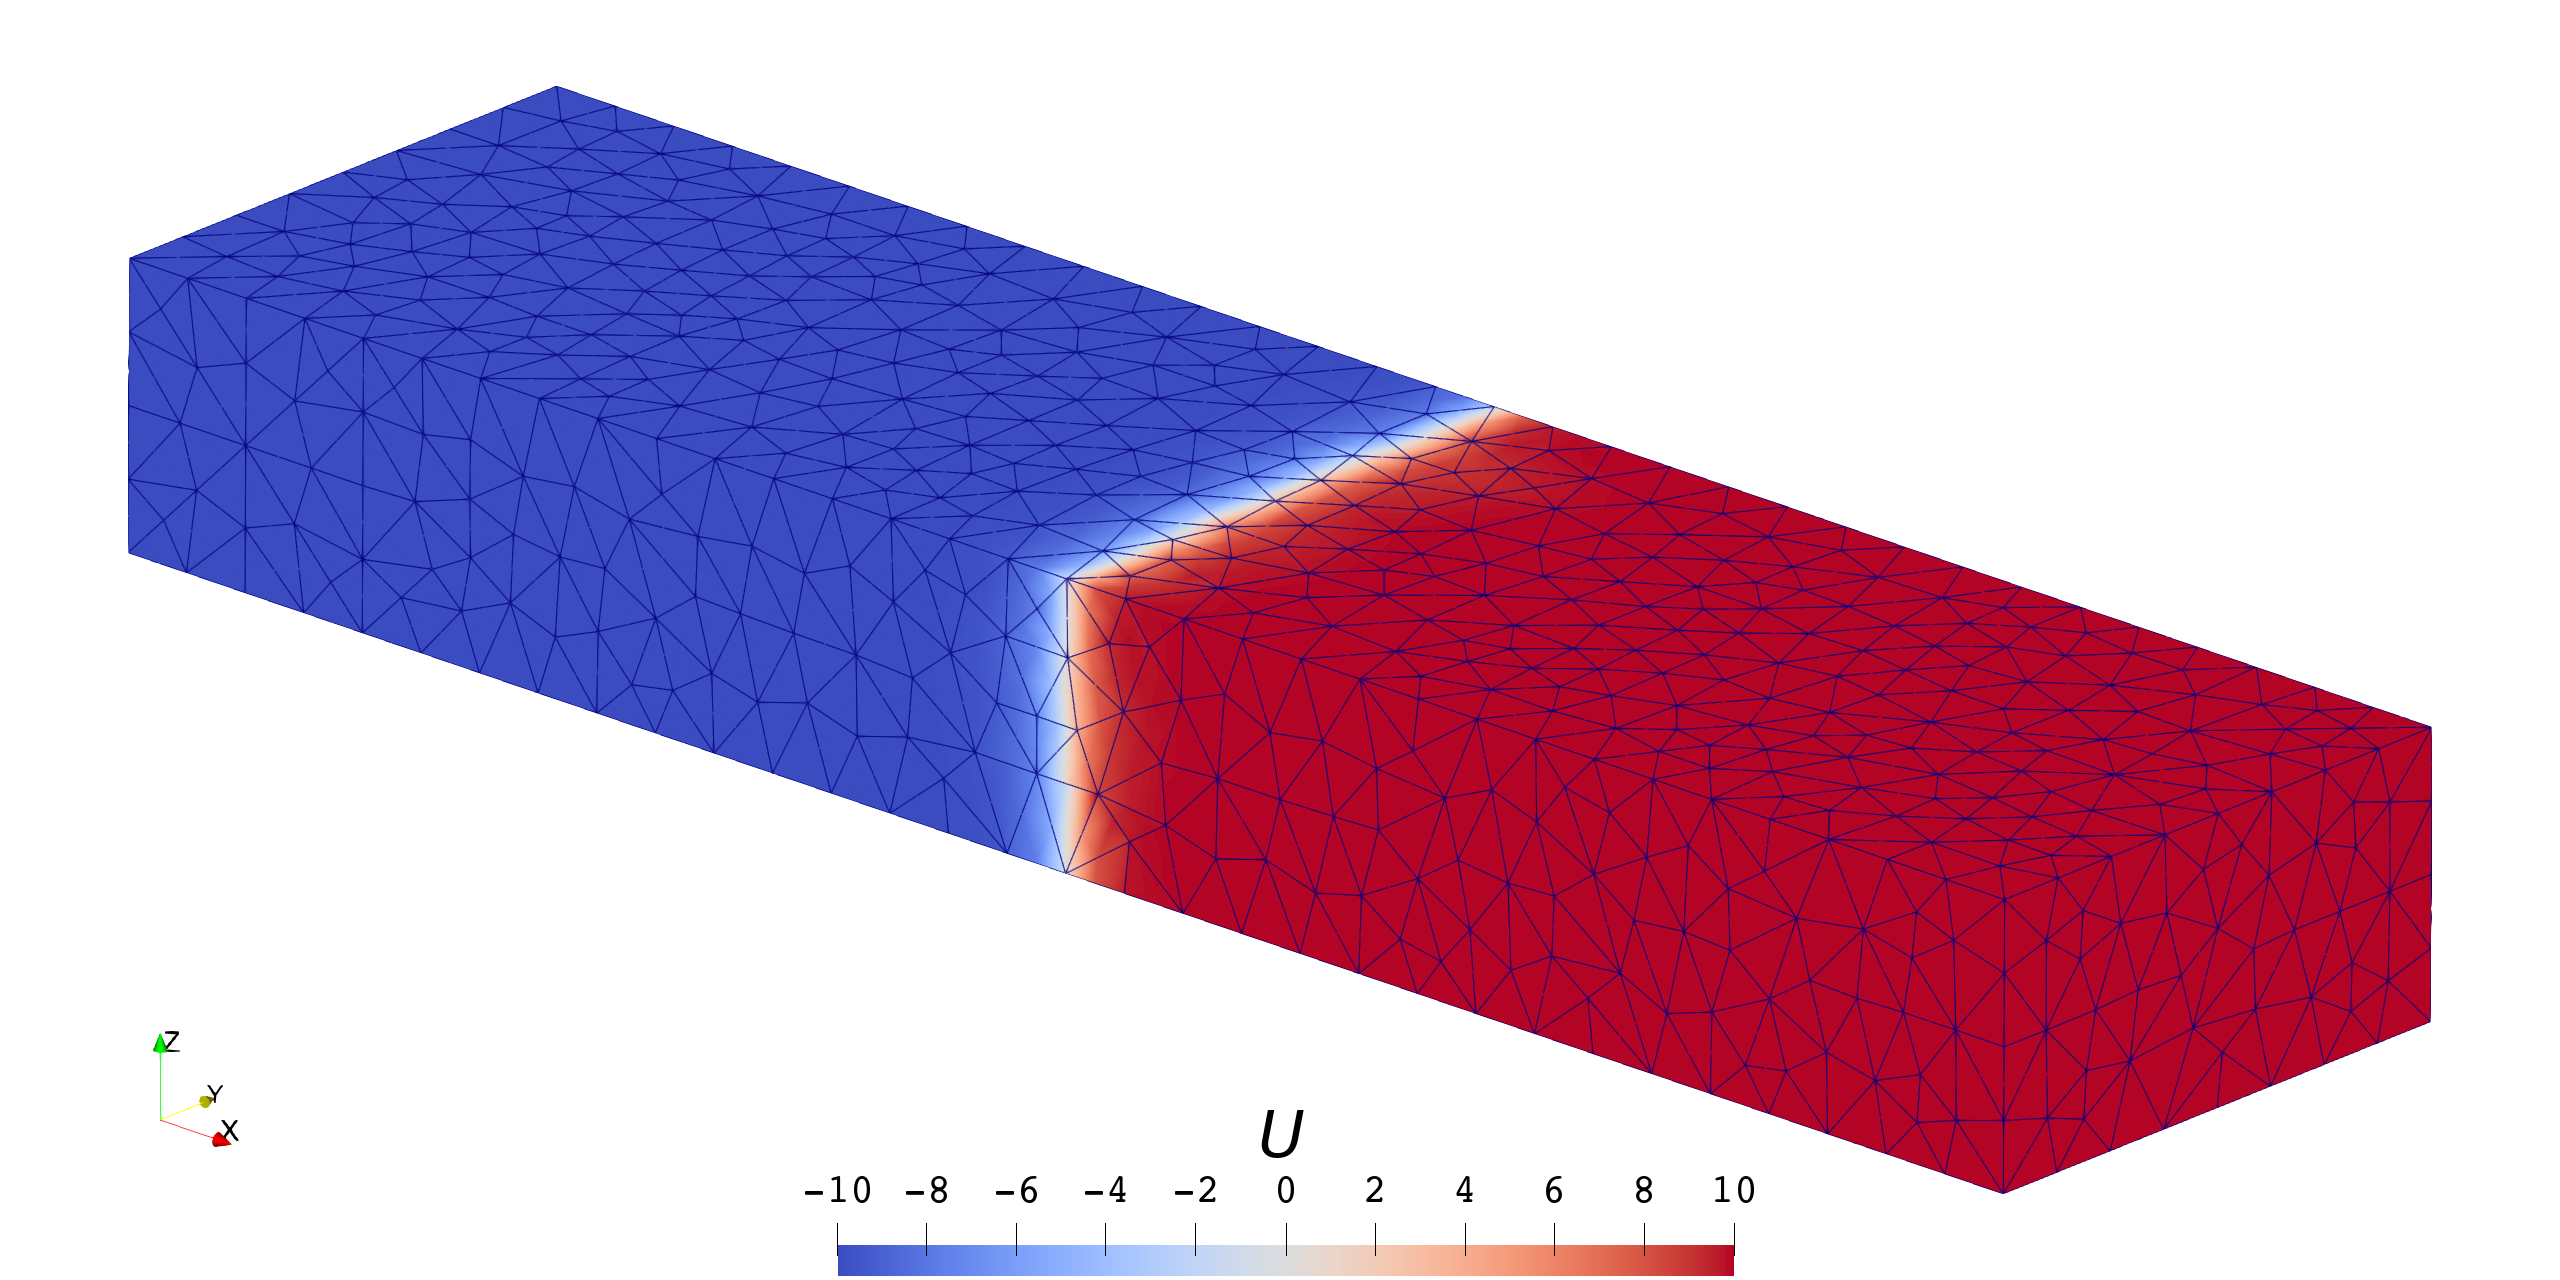
\includegraphics[width=0.99\textwidth]{figures/linear_scalar/p=3_h=2^-3}

\caption{\label{fig:linear_scalar_p=00003D3_h=00003D2^-3}{Third-order solution}
of Problem \ref{prob:linear_scalar} on medium ($h\approx2^{-3}$)
cells.}%mdpi: please change -1.0e+01 format to scientific notation: -1.0 x 10^1, the same problem as the following figures
\end{figure}
\vspace{-12pt}

\begin{figure}[H]
\hspace{-1.5em}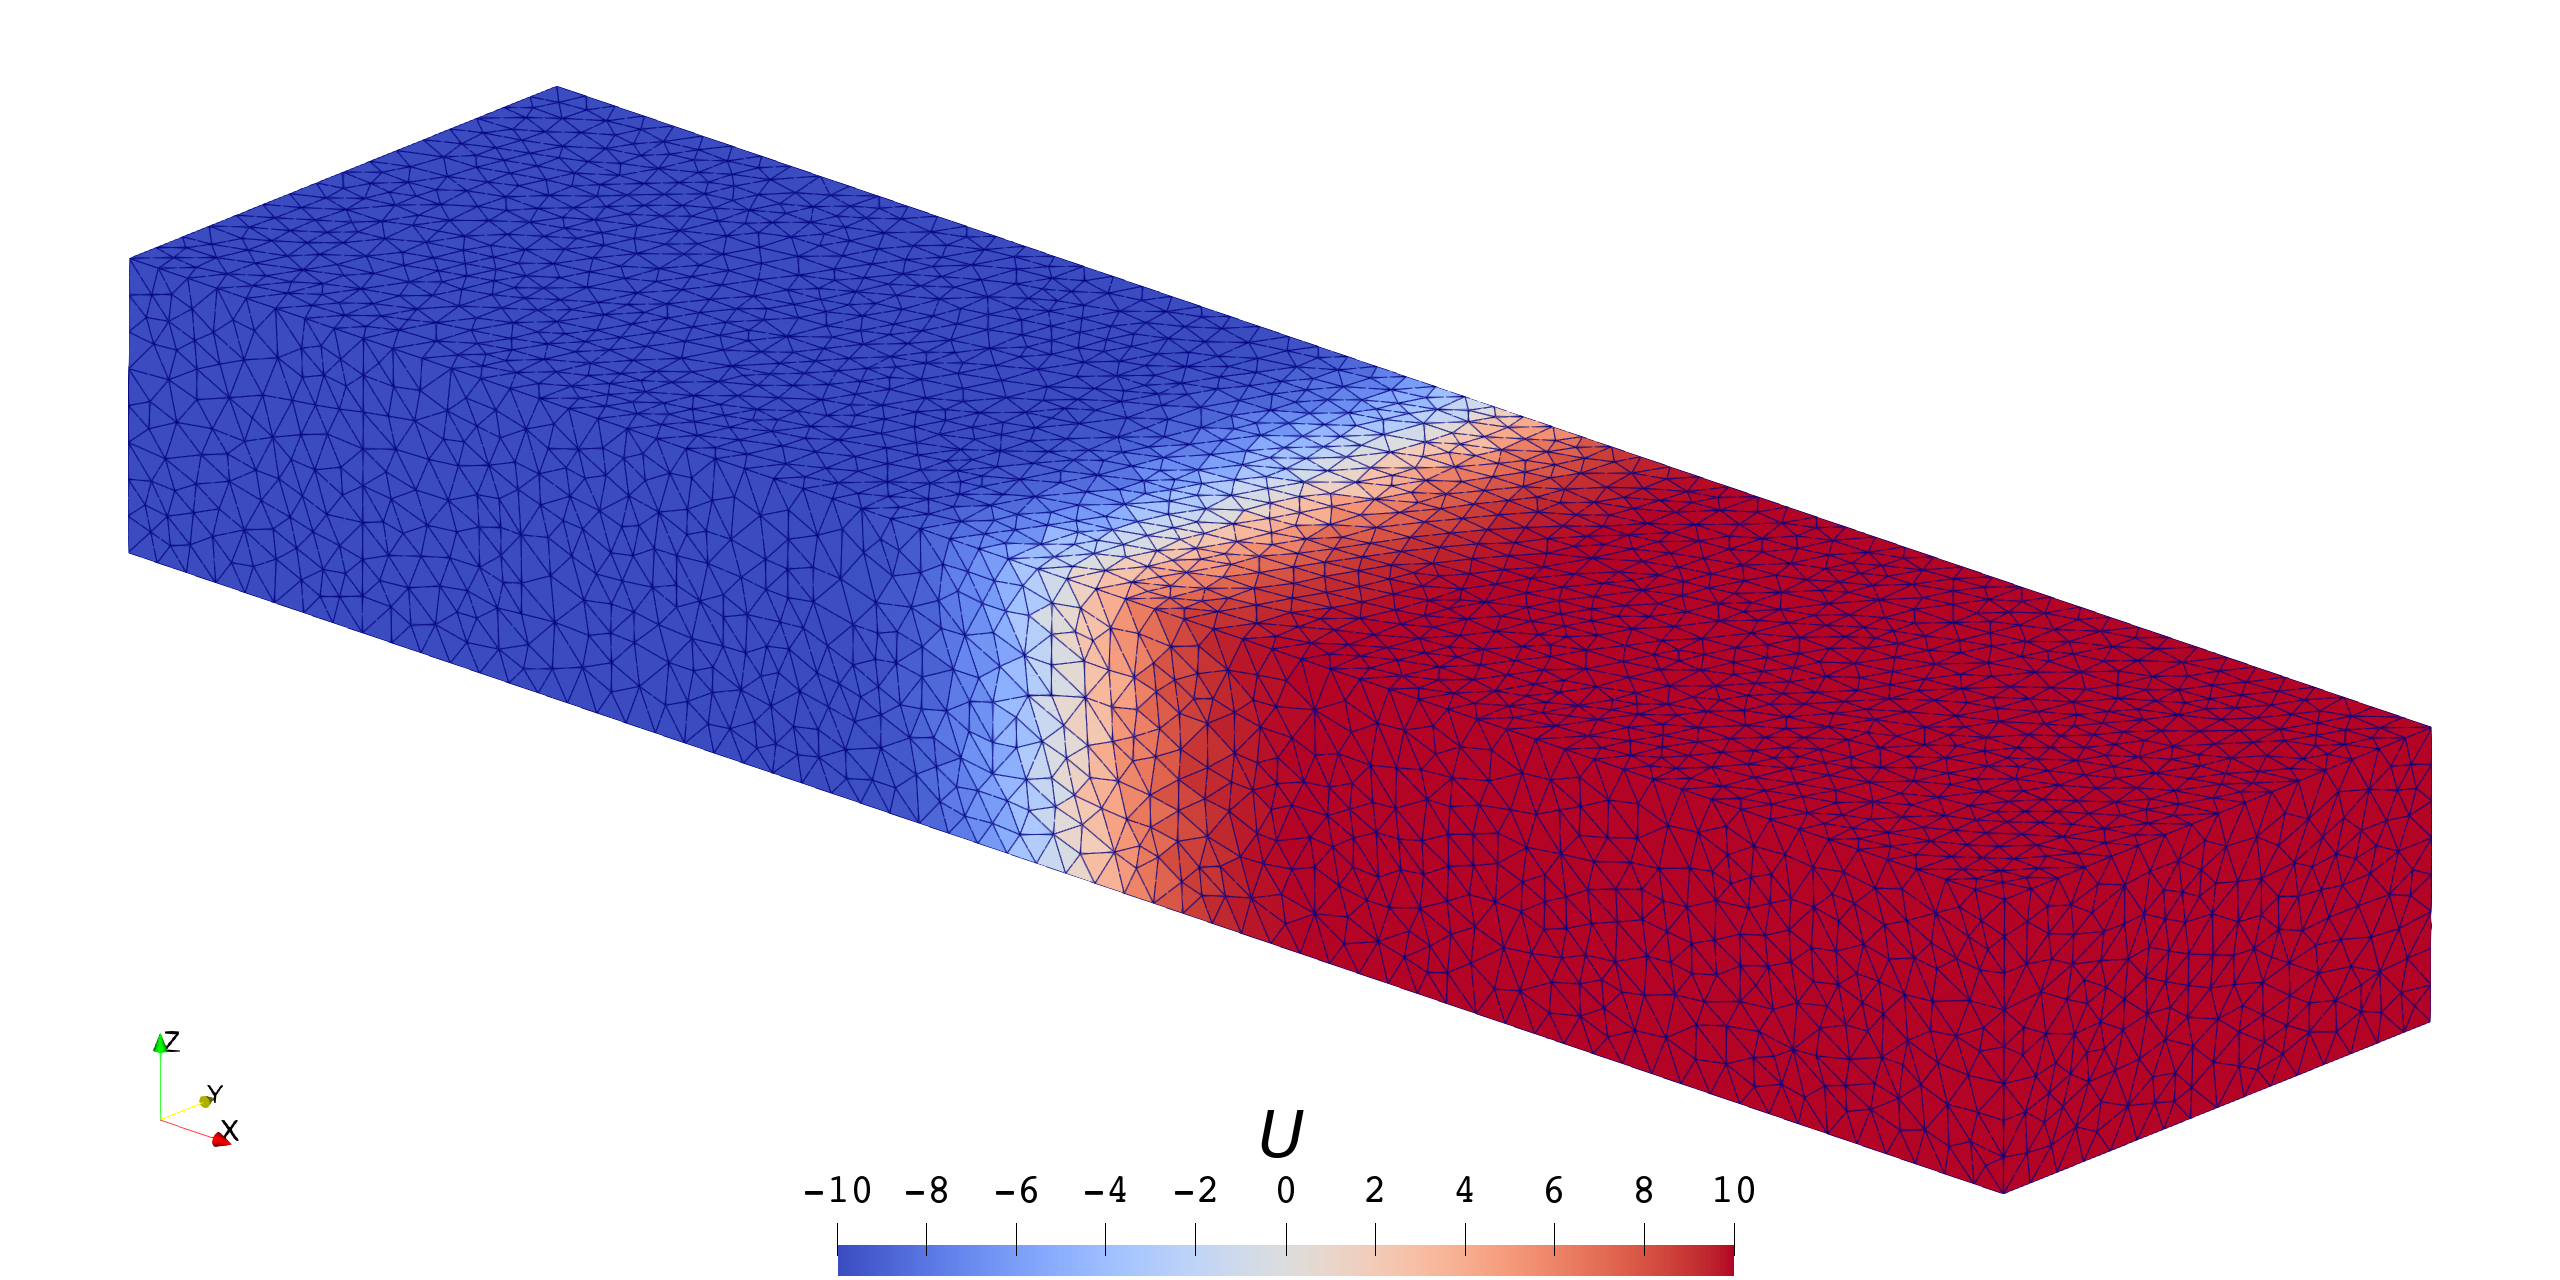
\includegraphics[width=0.99\textwidth]{figures/linear_scalar/p=1_h=2^-4}

\caption{\label{fig:linear_scalar_p=00003D1_h=00003D2^-4}{First-order solution}
of Problem \ref{prob:linear_scalar} on small ($h\approx2^{-4}$)
cells.}
\end{figure}
\vspace{-12pt}
\begin{figure}[H]
\hspace{-1.5em}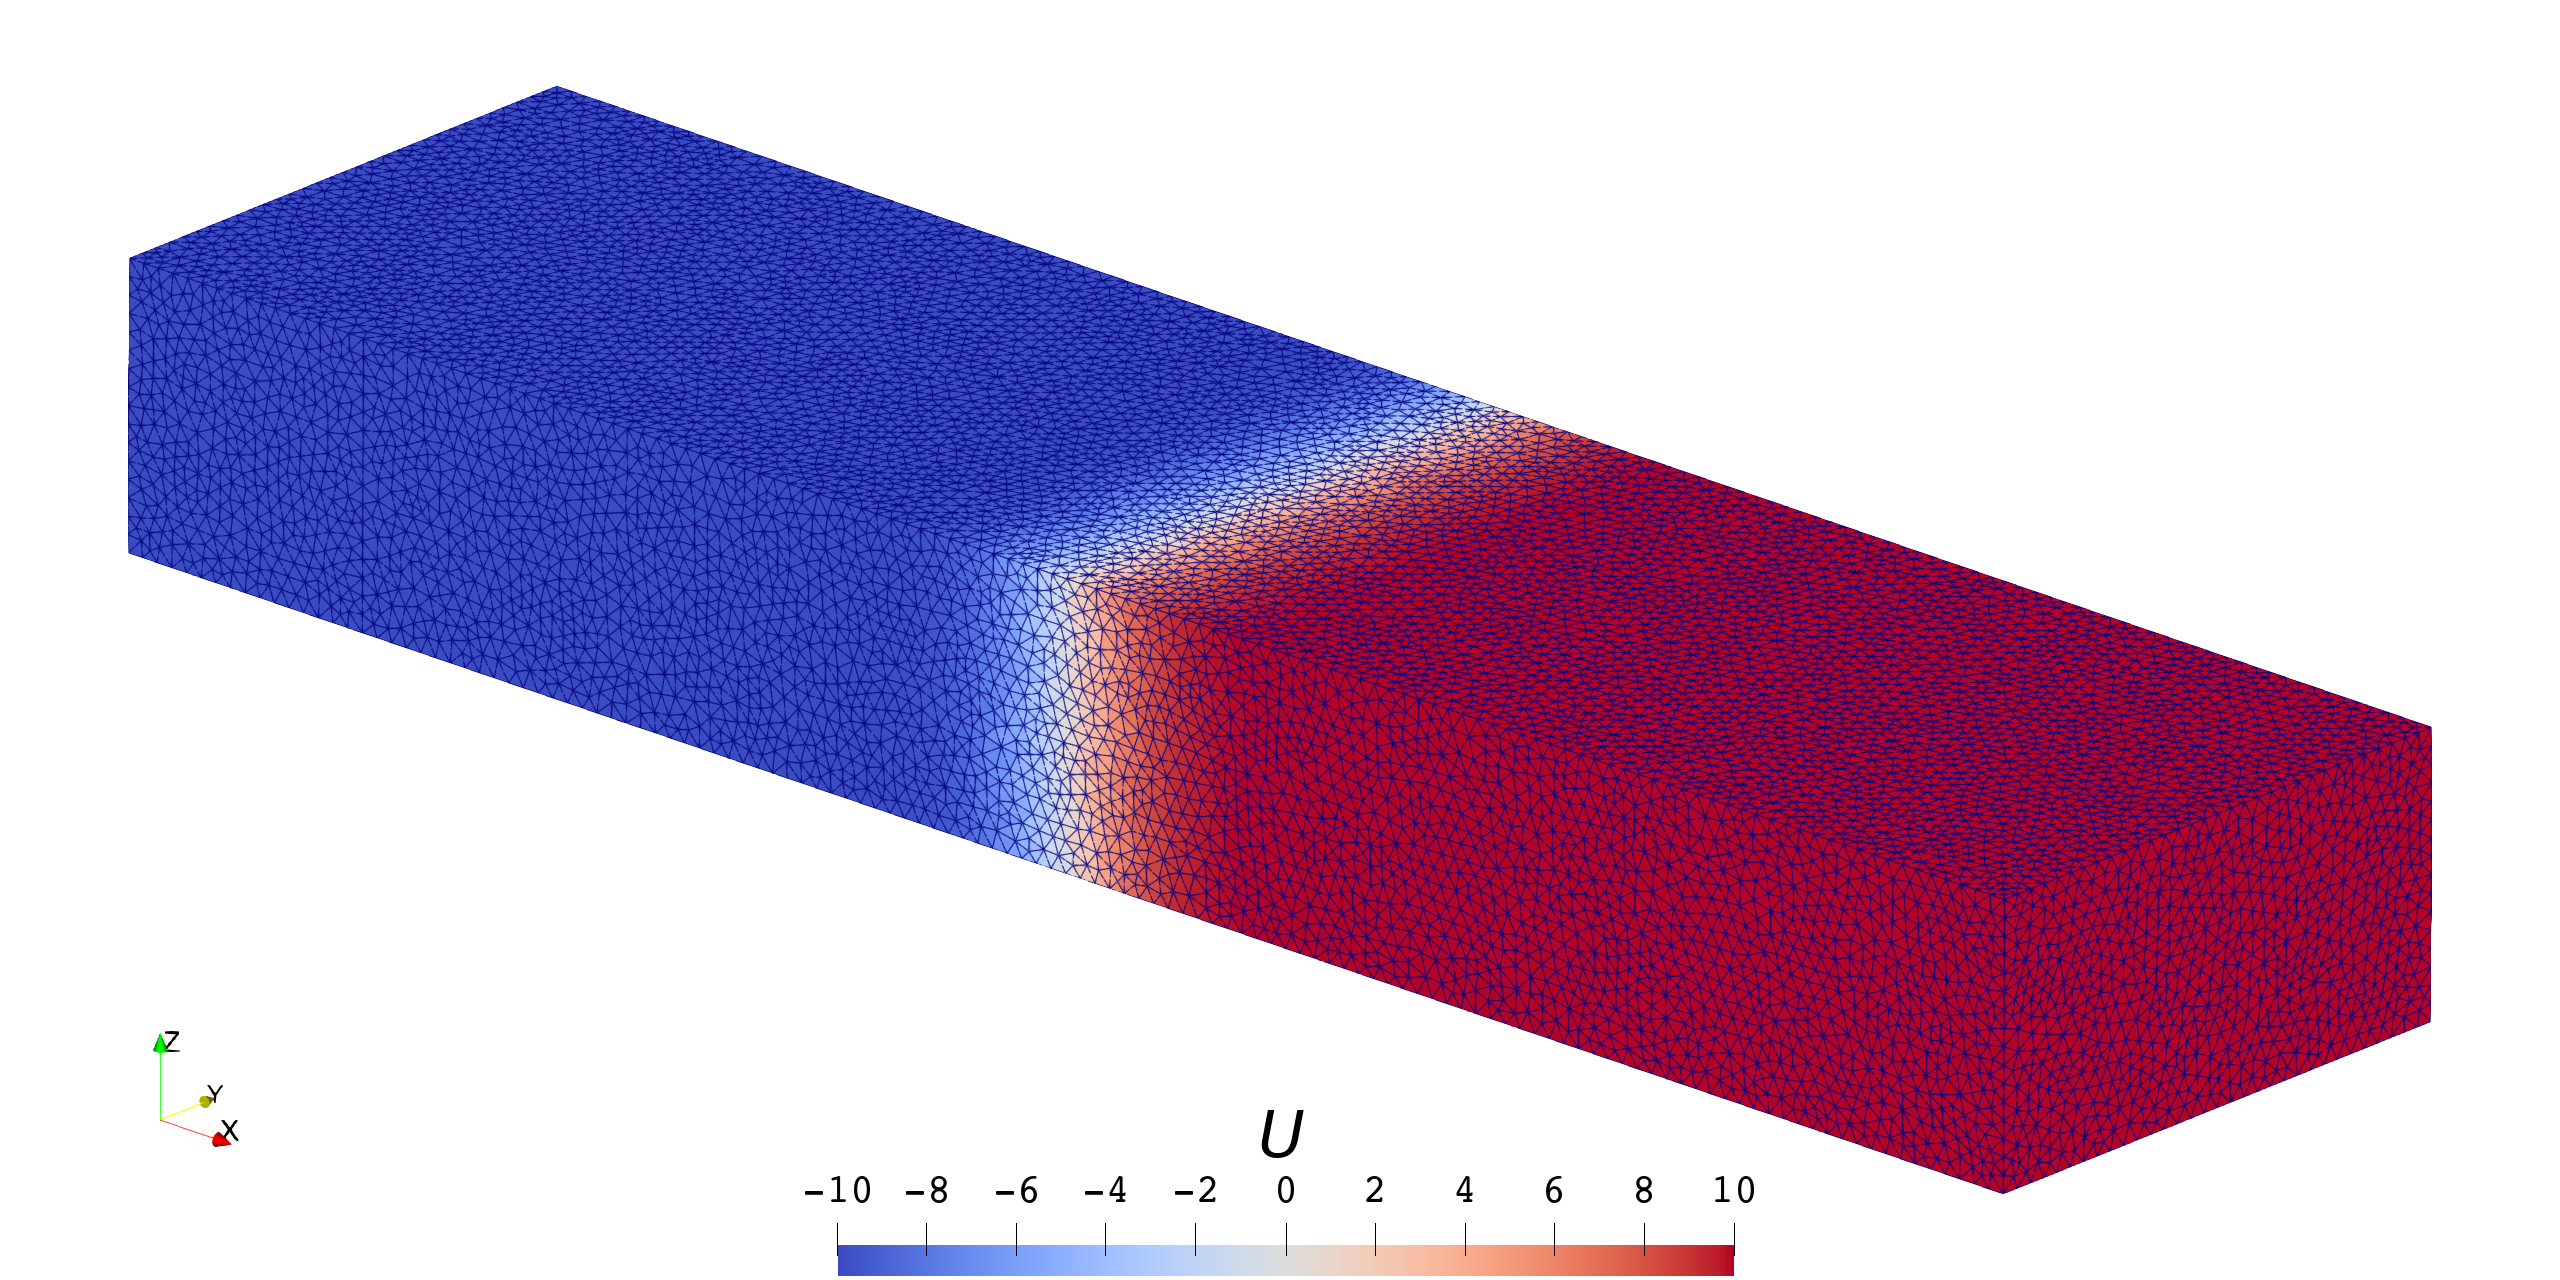
\includegraphics[width=0.99\textwidth]{figures/linear_scalar/p=1_h=2^-5}

\caption{\label{fig:linear_scalar_p=00003D1_h=00003D2^-5}{First-order solution}
of Problem \ref{prob:linear_scalar} on tiny ($h\approx2^{-5}$) cells.}
\end{figure}
\vspace{-12pt}
\begin{figure}[H]
\hspace{-1.5em}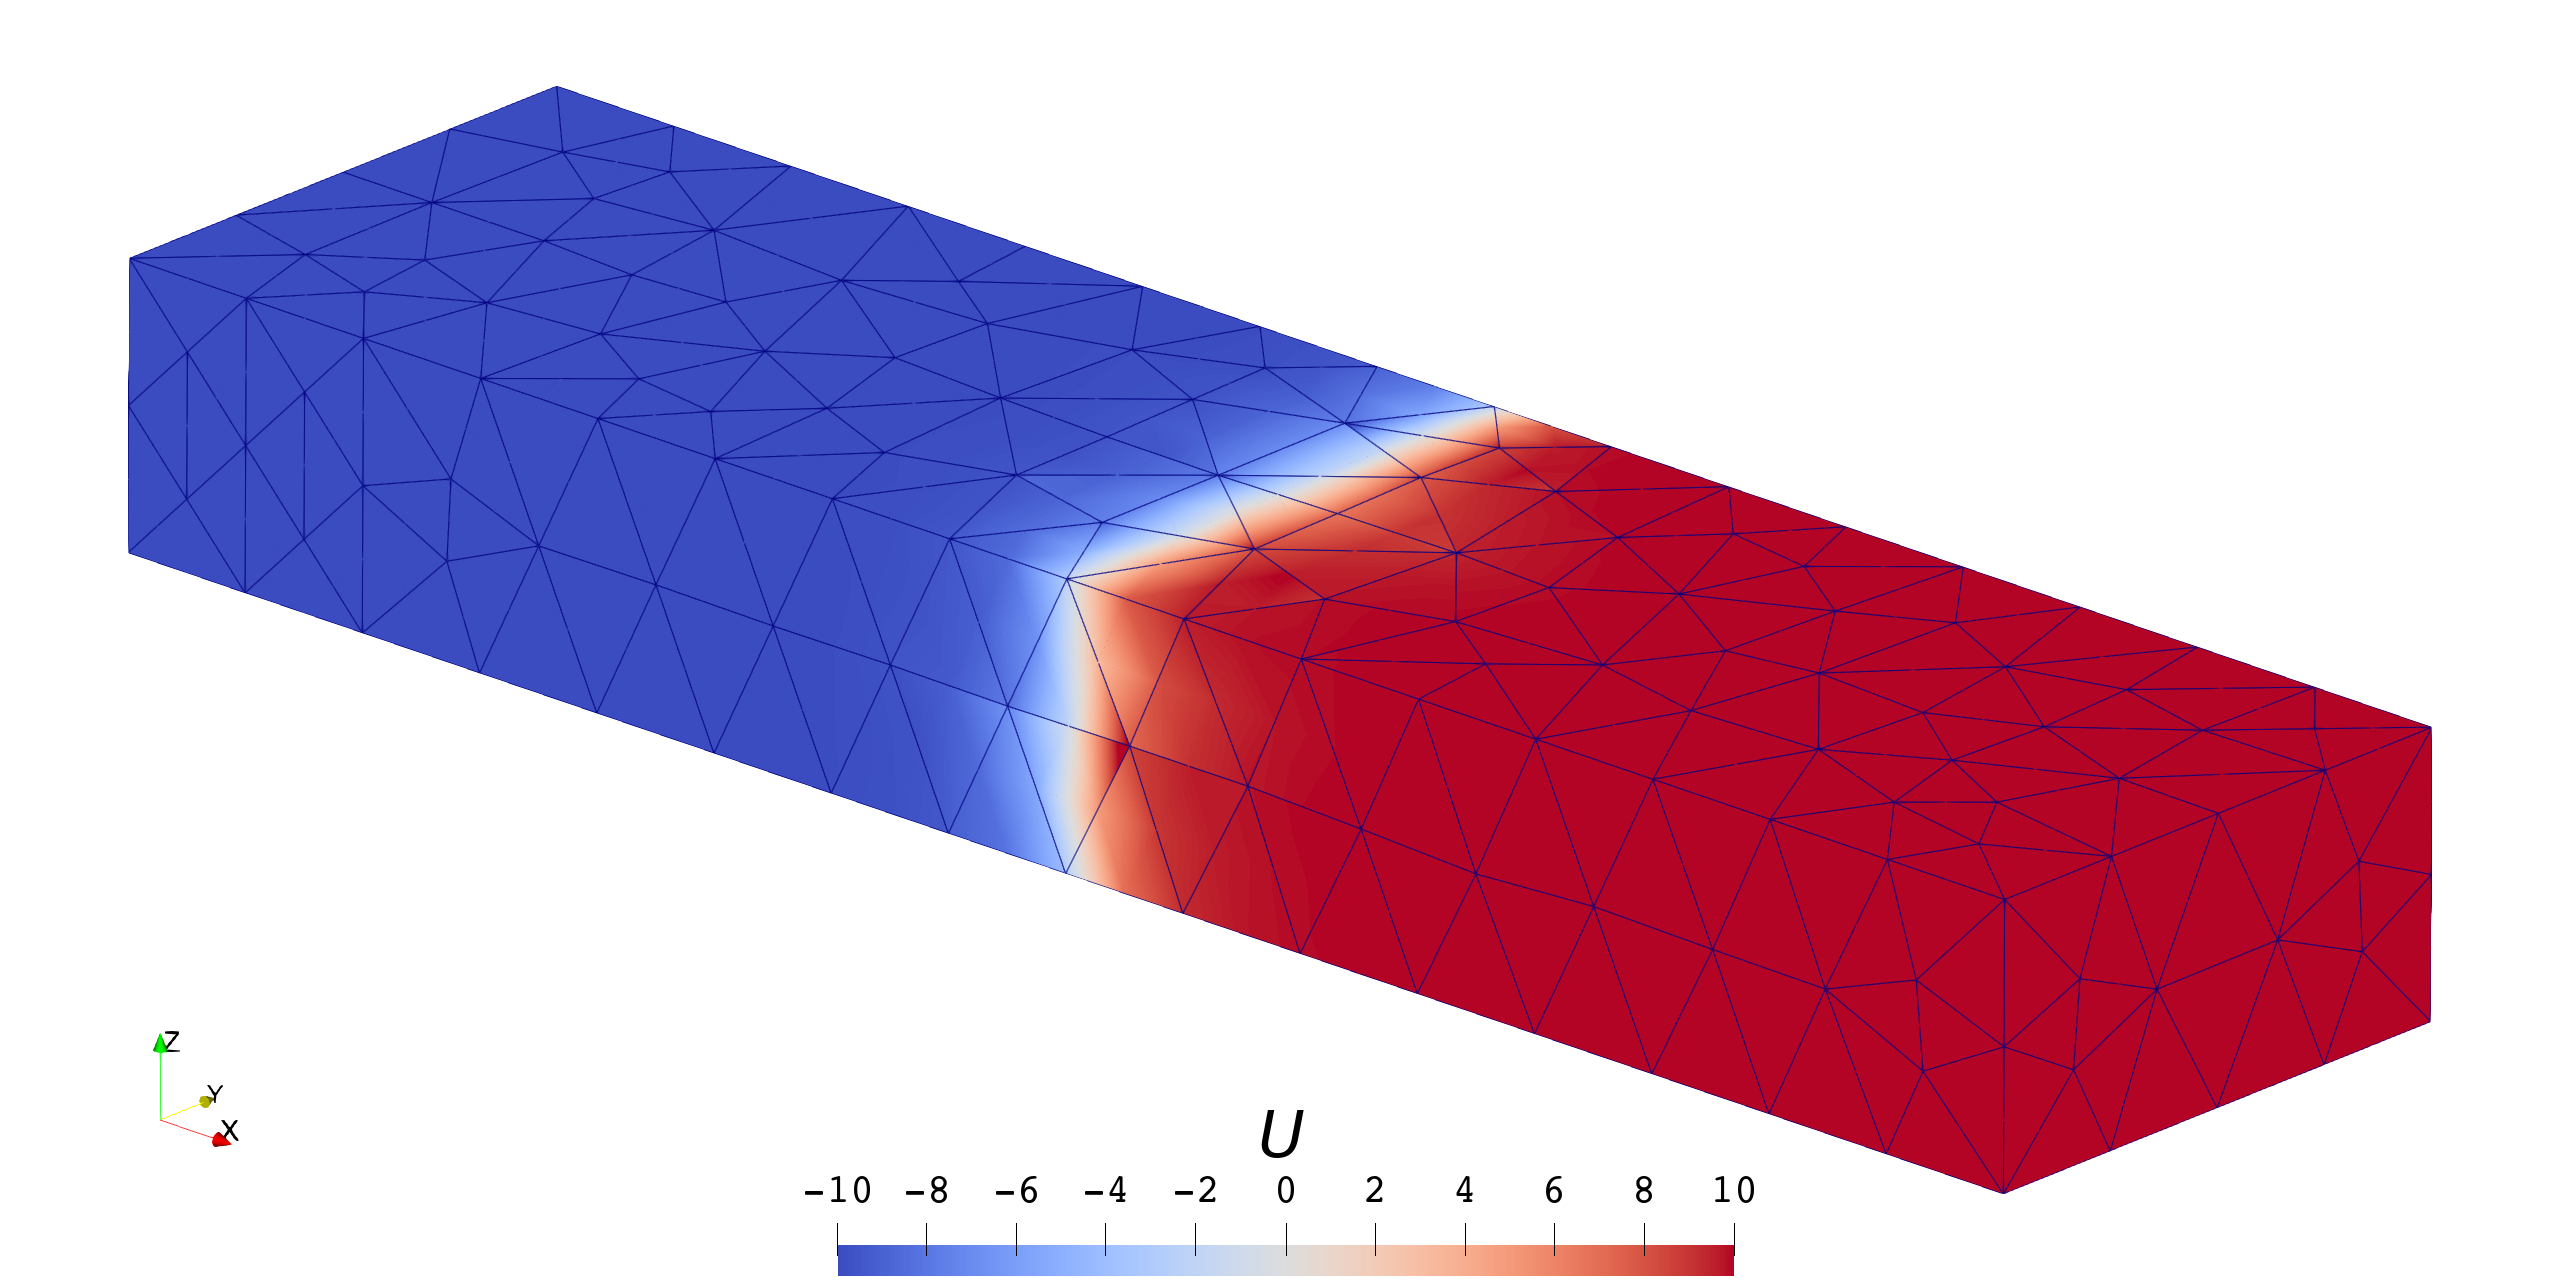
\includegraphics[width=0.99\textwidth]{figures/linear_scalar/p=3_h=2^-2}
%\vspace{-6pt}
\caption{\label{fig:linear_scalar_p=00003D3_h=00003D2^-2}{Third-order solution}
of Problem \ref{prob:linear_scalar} on big ($h\approx2^{-2}$) cells.}
\end{figure}
\vspace{-12pt}
\begin{figure}[H]
\hspace{-1em}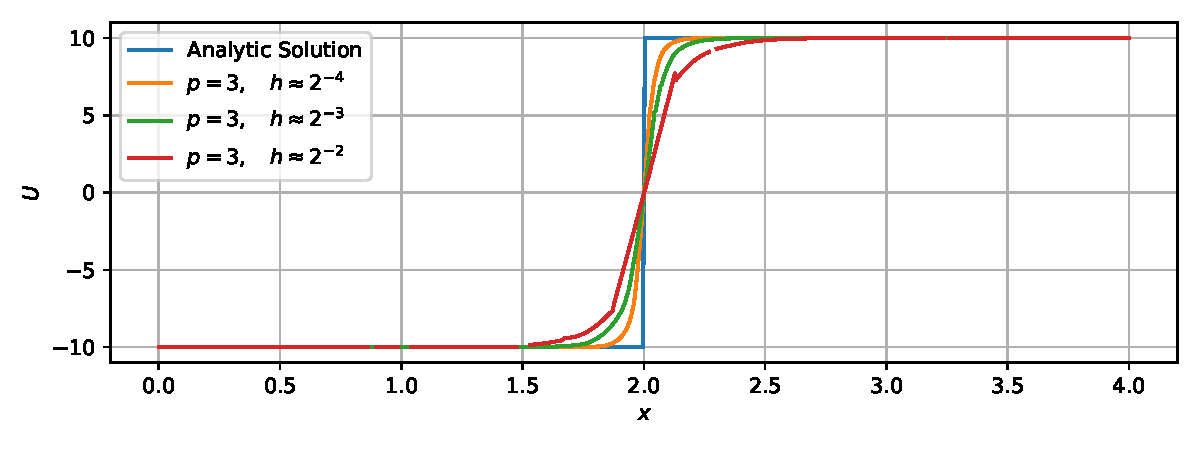
\includegraphics[width=0.99\textwidth]{figures/linear_scalar/h_vary}

\caption{\label{fig:linear_scalar_h_vary}Comparison between solutions of Problem
\ref{prob:linear_scalar} given by running the same solver on \mbox{different
meshes.}}
\end{figure}
\vspace{-12pt}
\begin{figure}[H]
\hspace{-0.7em}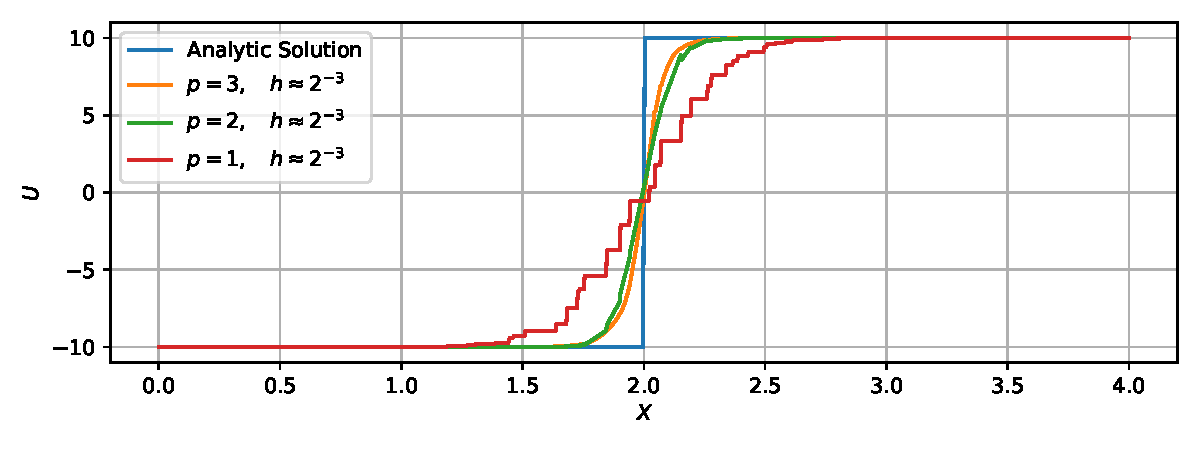
\includegraphics[width=0.99\textwidth]{figures/linear_scalar/p_vary}

\caption{\label{fig:linear_scalar_p_vary}Comparison between solutions of Problem
\ref{prob:linear_scalar} given by running different solvers on the
\mbox{same mesh.}}
\end{figure}

In Table \ref{tab:accuracy_and_cost}, we show the measured error
and time cost of each solver/mesh pair. The seconds consumed by first-order
solutions are somewhat exaggerated, since we use the same high-order
quadrature rules for both first- and third-order solvers, which is
necessary to integrate non-constant errors. If we did not have to
measure the errors, then low-order numerical integrators could be
used, which might save some time.

\begin{table}[H]
\caption{{Accuracy and} time cost of each solver--mesh ($p$--$h$) pair.\label{tab:accuracy_and_cost}}%mdpi: we changed the table format, please confirm it  // OK, thanks.
\newcolumntype{C}{>{\centering\arraybackslash}X}
\begin{tabularx}{\textwidth}{CCCCC}
\toprule 
\multicolumn{5}{c}{\boldmath{$L_{1}$}\textbf{-Error with Respect to the Analytic Solution}}\\ \midrule
\diagbox[width=2.9cm, height=0.4cm]{\boldmath{$p$}}{\boldmath{$h$}} & \boldmath{$2^{-2}$} & \boldmath{$2^{-3}$} & \boldmath{$2^{-4}$} &\boldmath{ $2^{-5}$}\\
\midrule
1 & 2.858 & 2.095 & 1.524 & 1.108\\
2 & 1.258 & 0.771 & 0.463 & 0.275\\
3 & 1.021 & 0.590 & 0.341 & \\\midrule
\multicolumn{5}{c}{\textbf{Time Cost (in Seconds) Measured on a Single Core Whose Main Frequency Is 2.7 GHz}}\\\midrule
\diagbox[width=2.9cm, height=0.4cm]{\boldmath{$p$}}{\boldmath{$h$}} & \boldmath{$2^{-2}$} & \boldmath{$2^{-3}$} & \boldmath{$2^{-4}$} & \boldmath{$2^{-5}$}\\\midrule
1 & 0.373 & 1.129 & 16.533 & 306.293\\
2 & 1.580 & 14.894 & 253.821 & 4986.391 %MDPI: The dot should be removed? please confirm.  // The number of digits after the decimal point has been unified to be three.
\\
3 & 4.147 & 61.425 & 906.914 & \\


\bottomrule

\end{tabularx}
\end{table}


%\begin{minipage}[t]{0.49\textwidth}%
%
%
%
%
%\begin{tabular*}{1\textwidth}{@{\extracolsep{\fill}}>{\centering}p{0.2\textwidth}>{\centering}p{0.12\textwidth}>{\centering}p{0.12\textwidth}>{\centering}p{0.12\textwidth}>{\centering}p{0.12\textwidth}}
%
%\end{tabular*}%
%\end{minipage}\hfill{}%
%\begin{minipage}[t]{0.49\textwidth}%
%
%
%
%
%\begin{tabular*}{1\textwidth}{@{\extracolsep{\fill}}>{\centering}p{0.2\textwidth}>{\centering}p{0.12\textwidth}>{\centering}p{0.12\textwidth}>{\centering}p{0.12\textwidth}>{\centering}p{0.12\textwidth}}
%\toprule 
%\diagbox{$p$}{$h$} & $2^{-2}$ & $2^{-3}$ & $2^{-4}$ & $2^{-5}$\tabularnewline
%\midrule
%1 & 0.373 & 1.129 & 16.53 & 306.3\tabularnewline
%2 & 1.580 & 14.89 & 253.8 & 4986.\tabularnewline
%3 & 4.147 & 61.42 & 906.9 & \tabularnewline
%\bottomrule
%\end{tabular*}%
%\end{minipage}
%\end{table}

The following conclusions can be drawn from both Figures \ref{fig:linear_scalar_p=00003D3_h=00003D2^-3}--\ref{fig:linear_scalar_p_vary}
and Table \ref{tab:accuracy_and_cost}:
\begin{itemize}
\item Both mesh refinement (decreasing $h$) and order increment (increasing
$p$) can help to improve accuracy.
\item The solver of the highest order ($p=3$) on the coarsest ($h\approx2^{-2}$)
mesh defeats the solver of the lowest order ($p=1$) on the finest
($h\approx2^{-5}$) mesh in accuracy but saves quite a lot of time.
\item High-order schemes are better than low-order ones in the sense of
getting the same level of accuracy with less time cost.
\end{itemize}
%

\subsubsection{System Case}
\begin{Problem}
\label{prob:linear_system}In Equation (\ref{eq:linear_system}), let
$\underline{U}$ consists two components and each $\underline{A}$
be a $2\times2$ matrix:
\[
\underline{U}(\vec{x},t)=\begin{bmatrix}U_{1}(x,y,z,t)\\
U_{2}(x,y,z,t)
\end{bmatrix},\qquad\underline{A^{x}}=\begin{bmatrix}6 & -2\\
-2 & 6
\end{bmatrix},\qquad\underline{A^{y}}=\underline{A^{z}}=\begin{bmatrix}0 & 0\\
0 & 0
\end{bmatrix},
\]

The following boundary conditions
\[
\underline{U}(x=0,y,z,t)=\begin{bmatrix}0\\
0
\end{bmatrix}\eqqcolon\underline{U}_{\mathrm{L}},\qquad\underline{U}(x=4,y,z,t)=\begin{bmatrix}12\\
-4
\end{bmatrix}\eqqcolon\underline{U}_{\mathrm{R}},
\]
and the initial condition
\[
\underline{U}(x,y,z,t=0)=\underline{U}_{\mathrm{R}}
\]
are applied.
\end{Problem}

To solve this problem analytically, we first obtain the eigenvalue decomposition
of $\underline{A^{x}}$, which is
\[
\underbrace{\begin{bmatrix}6 & -2\\
-2 & 6
\end{bmatrix}}_{\underline{A^{x}}}=\underbrace{\begin{bmatrix}1 & 1\\
-1 & 1
\end{bmatrix}}_{\underline{R^{x}}}\underbrace{\begin{bmatrix}8\\
 & 4
\end{bmatrix}}_{\underline{\varLambda^{x}}}\underbrace{\begin{bmatrix}1/2 & -1/2\\
1/2 & 1/2
\end{bmatrix}}_{(\underline{R^{x}})^{-1}}
\]

By introducing the characteristic variable $\underline{V}\coloneqq(\underline{R^{x}})^{-1}\underline{U}$,
which means
\[
\begin{bmatrix}V_{1}\\
V_{2}
\end{bmatrix}\coloneqq\begin{bmatrix}1/2 & -1/2\\
1/2 & 1/2
\end{bmatrix}\begin{bmatrix}U_{1}\\
U_{2}
\end{bmatrix}=\frac{1}{2}\begin{bmatrix}U_{1}-U_{2}\\
U_{1}+U_{2}
\end{bmatrix},
\]
the boundary conditions become
\[
\underline{V}_{\mathrm{L}}=(\underline{R^{x}})^{-1}\underline{U}_{\mathrm{L}}=\begin{bmatrix}0\\
0
\end{bmatrix},\qquad\underline{V}_{\mathrm{R}}=(\underline{R^{x}})^{-1}\underline{U}_{\mathrm{R}}=\begin{bmatrix}8\\
4
\end{bmatrix},
\]
and the system can be decoupled:
\[
\begin{bmatrix}\partial_{t}+8\partial_{x}\\
 & \partial_{t}+4\partial_{x}
\end{bmatrix}\begin{bmatrix}V_{1}\\
V_{2}
\end{bmatrix}=\begin{bmatrix}0\\
0
\end{bmatrix}.
\]

We can then solve these two scalar problems independently, which gives
\[
V_{1}(x,y,z,t)=\begin{cases}
0 & x<8t\\
8 & x>8t
\end{cases},\qquad V_{2}(x,y,z,t)=\begin{cases}
0 & x<4t\\
4 & x>4t
\end{cases}.
\]

The solution of Problem \ref{prob:linear_system} can be obtained
by $\underline{U}=\underline{R^{x}}\,\underline{V}$, which gives
\begin{equation}
\underline{U}(\vec{x},t)=\begin{bmatrix}V_{2}+V_{1}\\
V_{2}-V_{1}
\end{bmatrix}=\begin{cases}
\underline{U}_{\mathrm{L}} & x/t<4\\
\underline{U}_{\mathrm{M}} & x/t\in(4,8)\\
\underline{U}_{\mathrm{R}} & x/t>8
\end{cases},\label{eq:system_solution}
\end{equation}
where
\[
\underline{U}_{\mathrm{L}}=\begin{bmatrix}0\\
0
\end{bmatrix},\qquad\underline{U}_{\mathrm{M}}=\begin{bmatrix}4\\
4
\end{bmatrix},\qquad\underline{U}_{\mathrm{R}}=\begin{bmatrix}12\\
-4
\end{bmatrix}.
\]

With this analytic solution, we can evaluate the accuracy of our numerical
solvers. Four solver--limiter pairs are tested on the same mesh ($h\approx2^{-3}$)
used in Figure \ref{fig:linear_scalar_p=00003D3_h=00003D2^-3}.


\textls[-15]{We plot the contour of $\underline{U}(x,y,z,t=0.3)$ with the underlying
mesh in \mbox{{Figures} \ref{fig:linear_system_u_1_contour} and  \ref{fig:linear_system_u_2_contour}}%mdpi: Figure 9 citation before Figure 8, please change it, ensure the first citation of each figure appears in numerical order  // OK.
~and compare the results along the longitudinal axis at $t=0.3$ with
the analytic solution in \mbox{Figures \ref{fig:linear_system_u_1} and \ref{fig:linear_system_u_2}}.
It is clear that both \texttt{LazyWeno} and \texttt{EigenWeno} (see
Section \ref{subsec:limiting_procedures}) can essentially suppress
non-physical oscillations in each component. Figure \ref{fig:linear_system_error}
shows that higher-order ($p=3$) solvers still outperforms lower-order
($p=2$) solvers in accuracy and the \texttt{EigenWeno} limiter generally
works better than its \texttt{LazyWeno} counterpart. For this reason,
we will use \texttt{EigenWeno} limiters exclusively in the rest of
this section.}
\begin{figure}[H]
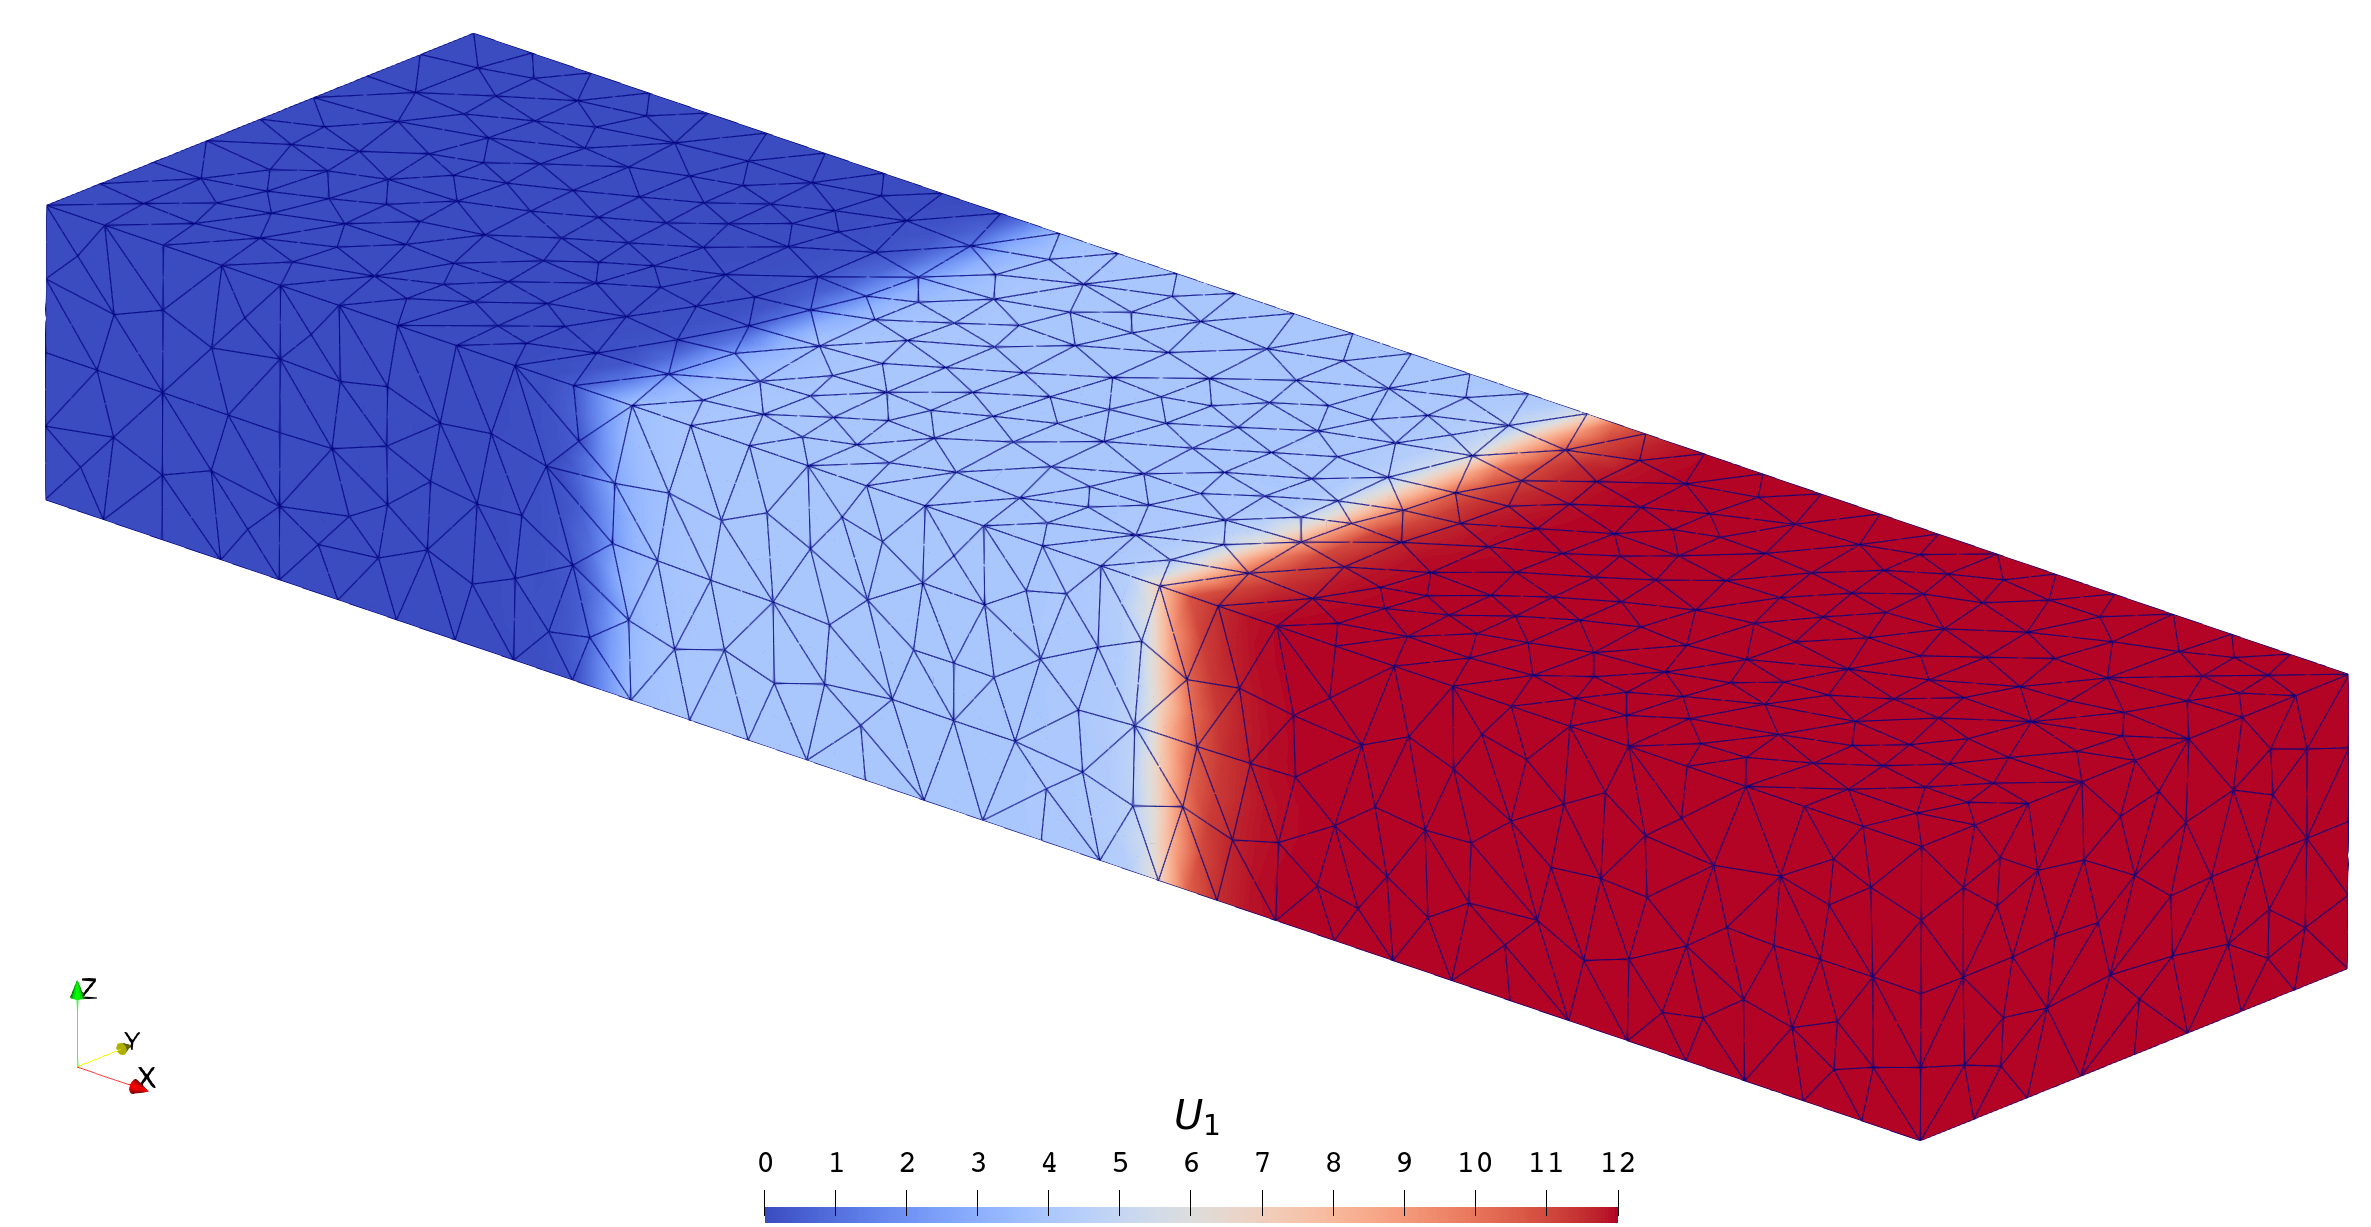
\includegraphics[width=0.99\textwidth]{figures/linear_system/u_1_contour}

\caption{\label{fig:linear_system_u_1_contour}{Third-order solution} of $U_{1}(t=0.3)$
in Problem \ref{prob:linear_system}.}
\end{figure}
\vspace{-12pt}
\begin{figure}[H]
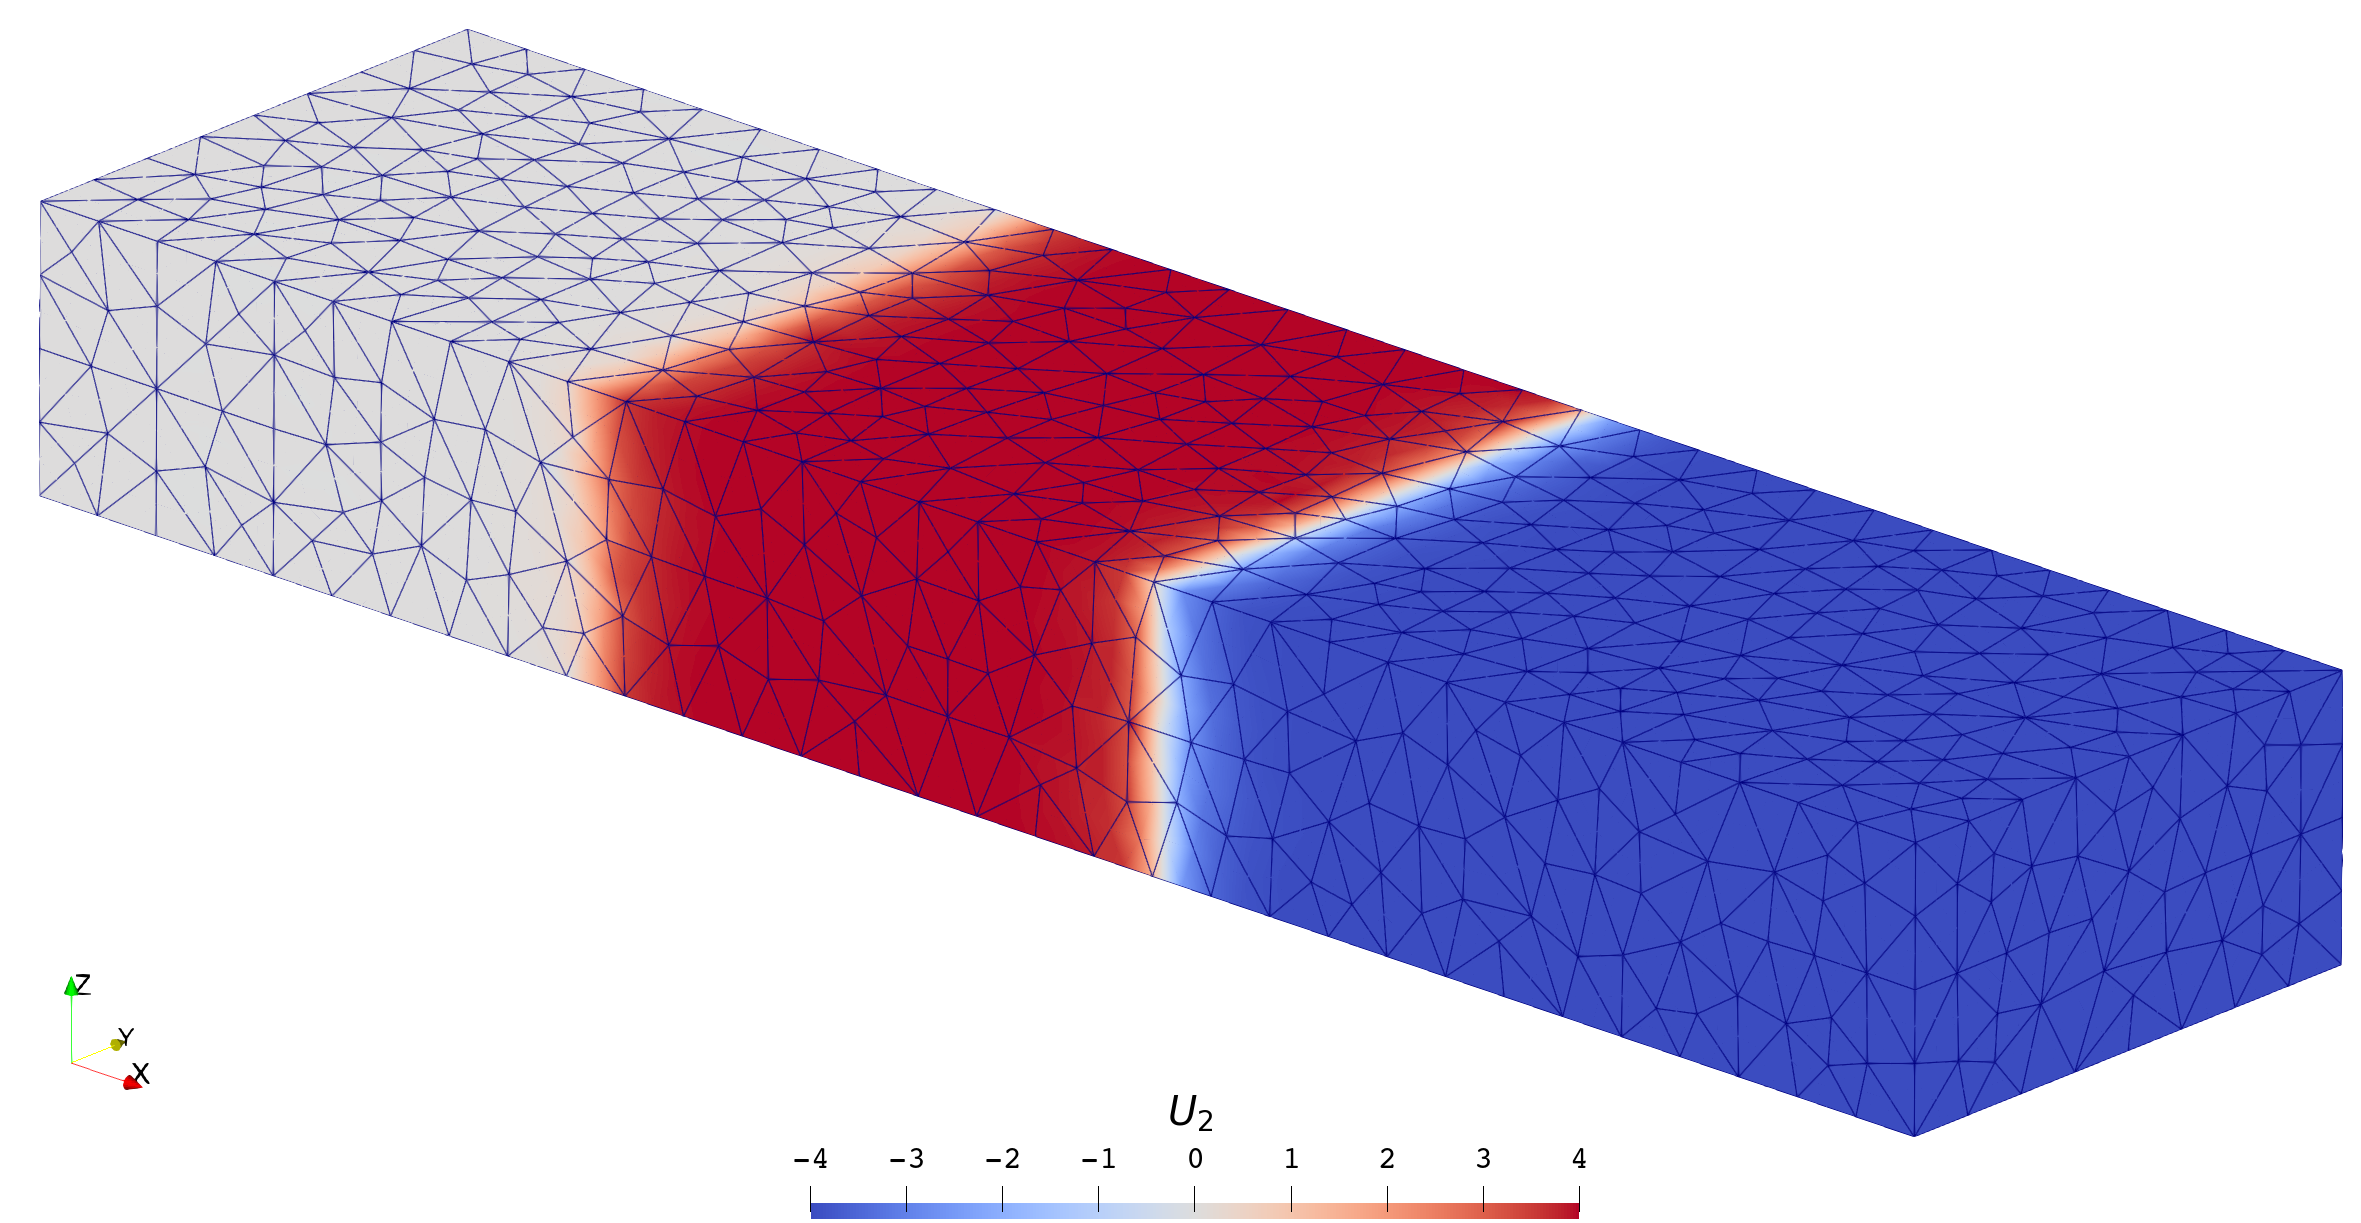
\includegraphics[width=0.99\textwidth]{figures/linear_system/u_2_contour}

\caption{\label{fig:linear_system_u_2_contour}{Third-order solution} of $U_{2}(t=0.3)$
in Problem \ref{prob:linear_system}.}%mdpi: please change hyphen to minus sign  // OK.
\end{figure}
\vspace{-12pt}
\begin{figure}[H]
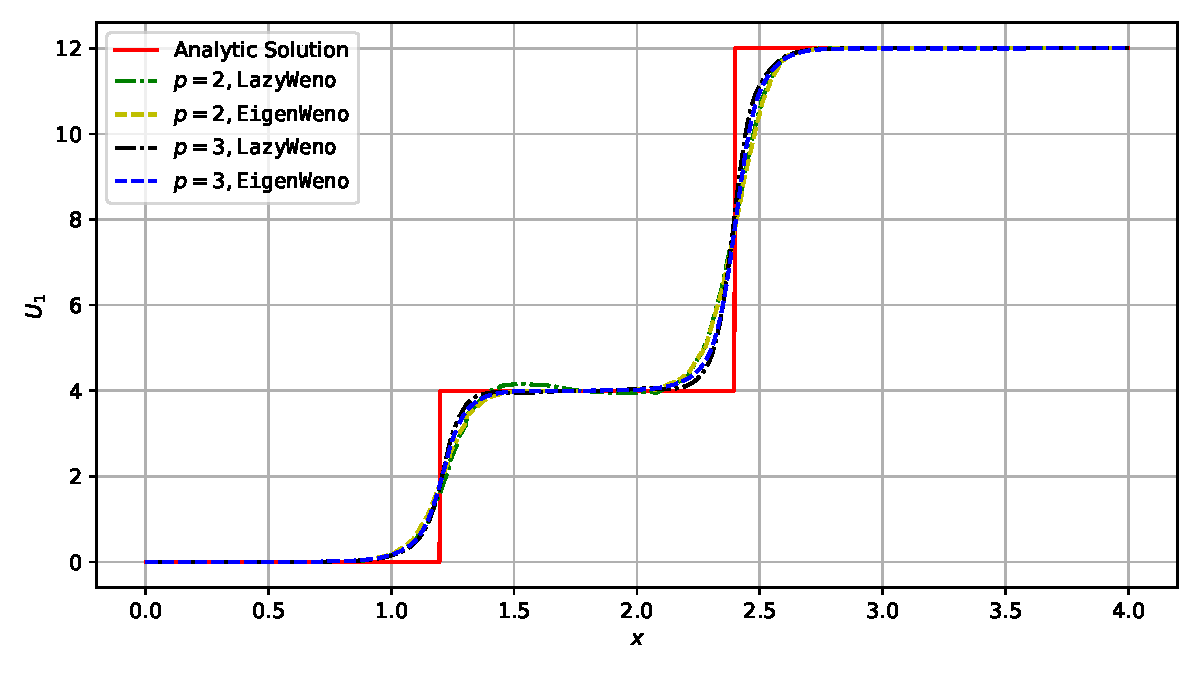
\includegraphics[width=0.99\textwidth]{figures/linear_system/u_1}

\caption{\label{fig:linear_system_u_1}Comparison between solutions of $U_{1}(t=0.3)$
in Problem \ref{prob:linear_system}.}
\end{figure}
\vspace{-12pt}
\begin{figure}[H]
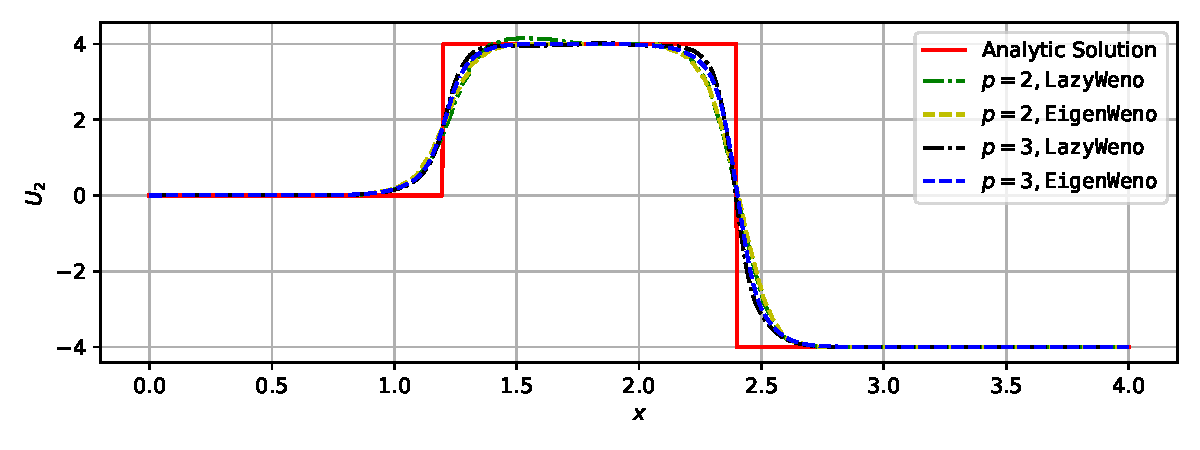
\includegraphics[width=0.99\textwidth]{figures/linear_system/u_2}

\caption{\label{fig:linear_system_u_2}Comparison between solutions of $U_{2}(t=0.3)$
in Problem \ref{prob:linear_system}.}
\end{figure}
\vspace{-12pt}


\begin{figure}[H]
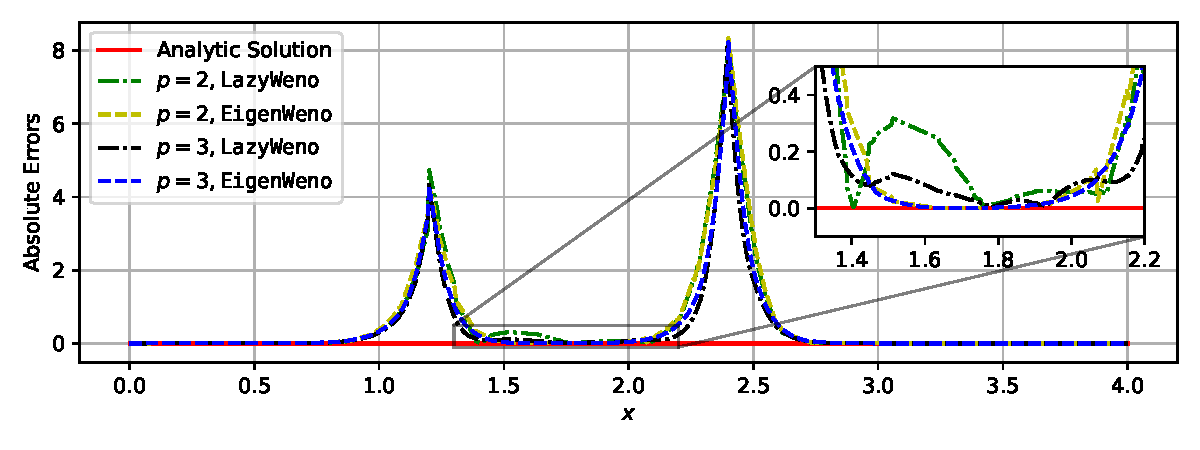
\includegraphics[width=0.99\textwidth]{figures/linear_system/error}

\caption{\label{fig:linear_system_error}Comparison between absolute errors
of numerical solutions in Figures \ref{fig:linear_system_u_1} and
\ref{fig:linear_system_u_2}.}
\end{figure}


\subsection{Inviscid Compressible Flows}

The second group of problems to be solved is the three-dimensional
Euler system:
\begin{equation}
\partial_{t}\begin{bmatrix}\rho\\
\rho u_{x}\\
\rho u_{y}\\
\rho u_{z}\\
\rho e_{0}
\end{bmatrix}+\partial_{x}\begin{bmatrix}\rho u_{x}\\
\rho u_{x}u_{x}+p\\
\rho u_{y}u_{x}\\
\rho u_{z}u_{x}\\
\rho h_{0}u_{x}
\end{bmatrix}+\partial_{y}\begin{bmatrix}\rho u_{y}\\
\rho u_{x}u_{y}\\
\rho u_{y}u_{y}+p\\
\rho u_{z}u_{y}\\
\rho h_{0}u_{y}
\end{bmatrix}+\partial_{z}\begin{bmatrix}\rho u_{z}\\
\rho u_{x}u_{z}\\
\rho u_{y}u_{z}\\
\rho u_{z}u_{z}+p\\
\rho h_{0}u_{z}
\end{bmatrix}=\begin{bmatrix}0\\
0\\
0\\
0\\
0
\end{bmatrix}\label{eq:euler_system}
\end{equation}
with certain boundary and initial conditions. These problems are genuinely
nonlinear which cannot be solved analytically in general. However,
their exact or high-order solutions in lower-dimensional spaces are
well known in CFD studies, which can still be used to test our
three-dimensional solvers.

\textls[-25]{For this system, the $\underline{A^{\nu}}$ defined in Equation (\ref{eq:normal_jacobian})
depends on $\underline{U}$, so do the $\underline{R}^{-1}$ in \mbox{Equation
(\ref{eq:eigen_cols})} and the $\underline{R}$ in Equation (\ref{eq:eigen_rows}).
Fortunately, these matrices can be \mbox{explicitly formulated:}}
\[
\underline{R}(\underline{U})=\begin{bmatrix}1 & 1 & 0 & 0 & 1\\
u_{x}-a\nu_{x} & u_{x} & \sigma_{x} & \pi_{x} & u_{x}+a\nu_{x}\\
u_{y}-a\nu_{y} & u_{y} & \sigma_{y} & \pi_{y} & u_{y}+a\nu_{y}\\
u_{z}-a\nu_{z} & u_{z} & \sigma_{z} & \pi_{z} & u_{z}+a\nu_{z}\\
h_{0}-u_{\nu}a & \frac{u_{x}^{2}+u_{y}^{2}+u_{z}^{2}}{2} & u_{\sigma} & u_{\pi} & h_{0}+u_{\nu}a
\end{bmatrix},\qquad\begin{bmatrix}u_{\nu}\\
u_{\sigma}\\
u_{\pi}
\end{bmatrix}=\begin{bmatrix}\nu_{x} & \sigma_{x} & \pi_{x}\\
\nu_{y} & \sigma_{y} & \pi_{y}\\
\nu_{z} & \sigma_{z} & \pi_{z}
\end{bmatrix}^{-1}\begin{bmatrix}u_{x}\\
u_{y}\\
u_{z}
\end{bmatrix},
\]
\[
\underline{L}(\underline{U})=\begin{bmatrix}\frac{1}{2}\left(B_{2}+\frac{u_{\nu}}{a}\right) & \frac{-1}{2}\left(B_{1}u_{x}+\frac{\nu_{x}}{a}\right) & \frac{-1}{2}\left(B_{1}u_{y}+\frac{\nu_{y}}{a}\right) & \frac{-1}{2}\left(B_{1}u_{z}+\frac{\nu_{z}}{a}\right) & \frac{1}{2}B_{1}\\
1-B_{2} & B_{1}u_{x} & B_{1}u_{y} & B_{1}u_{z} & -B_{1}\\
-u_{\sigma} & \sigma_{x} & \sigma_{y} & \sigma_{z} & 0\\
-u_{\pi} & \pi_{x} & \pi_{y} & \pi_{z} & 0\\
\frac{1}{2}\left(B_{2}-\frac{u_{\nu}}{a}\right) & \frac{-1}{2}\left(B_{1}u_{x}-\frac{\nu_{x}}{a}\right) & \frac{-1}{2}\left(B_{1}u_{y}-\frac{\nu_{y}}{a}\right) & \frac{-1}{2}\left(B_{1}u_{z}-\frac{\nu_{z}}{a}\right) & \frac{1}{2}B_{1}
\end{bmatrix},
\]
in which $B_{1}\coloneqq(\gamma-1)/a^{2}$ and $B_{2}\coloneqq B_{1}(u_{\nu}^{2}+u_{\sigma}^{2}+u_{\pi}^{2})$.

\subsubsection{Shock Tube Problems}

These problems are usually defined as one-dimensional problems, but
we treat them as three-dimensional ones. All these problems are considered
in a $[0.0,5.0]\times[0.0,1.0]\times[0.0,0.5]$ box with all boundaries
closed but the left and right ends open. Although no analytic solutions
exist, we can still use the method described in \citep{Toro_2009},
which solves nonlinear algebraic equations numerically, to obtain
their exact solutions. To test the numerical methods described in
Section \ref{sec:methods}, we use the unstructured hexahedral mesh
in Figure \ref{fig:shock_tube}, in which $h\approx1/10$.

\begin{figure}[H]
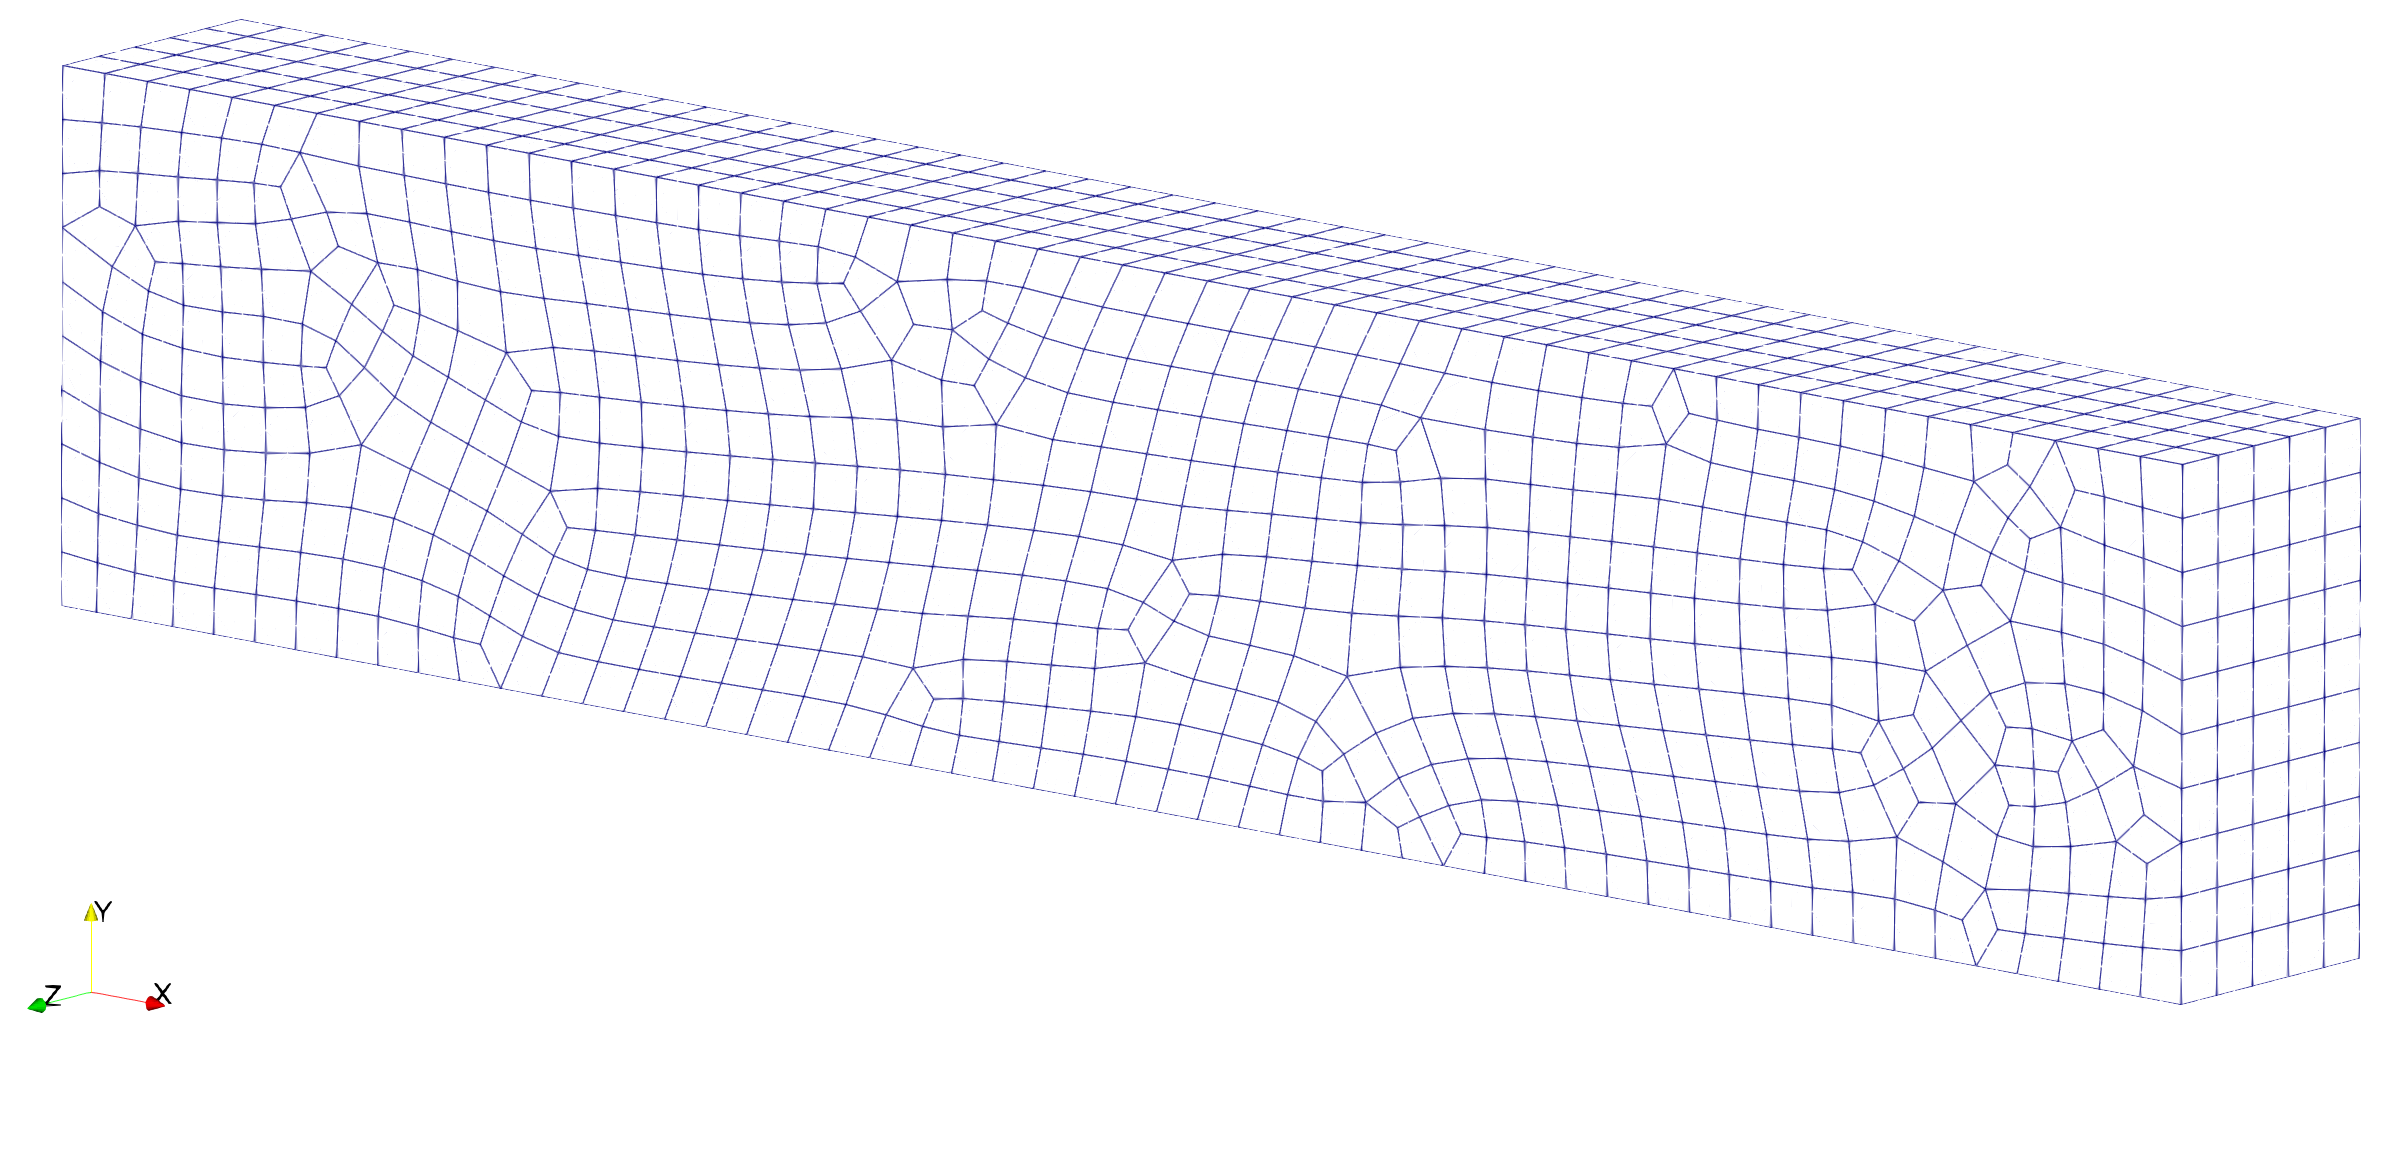
\includegraphics[width=0.99\textwidth]{figures/shock_tubes/mesh}

\caption{\label{fig:shock_tube}Mesh for Problems \ref{prob:sod}--\ref{prob:vacuum}.}
\end{figure}

\begin{Problem}
[Sod]\label{prob:sod}Solve the Euler system (Equation (\ref{eq:euler_system}))
for $t\in[0.0,1.0]$ with the initial condition
\[
\begin{bmatrix}\rho & u & vs. & w & p\end{bmatrix}_{t=0}=\begin{cases}
\begin{bmatrix}1.000 & 0.000 & 0.000 & 0.000 & 1.000\end{bmatrix} & x<2\\
\begin{bmatrix}0.125 & 0.000 & 0.000 & 0.000 & 0.100\end{bmatrix} & x>2
\end{cases}
\]
\end{Problem}

\begin{Problem}
[Lax]\label{prob:lax}Solve the Euler system (Equation (\ref{eq:euler_system}))
for $t\in[0.0,0.6]$ with the initial condition
\[
\begin{bmatrix}\rho & u & vs. & w & p\end{bmatrix}_{t=0}=\begin{cases}
\begin{bmatrix}0.445 & 0.698 & 0.000 & 0.000 & 3.528\end{bmatrix} & x<2\vspace{2pt}
\\
\begin{bmatrix}0.500 & 0.000 & 0.000 & 0.000 & 0.571\end{bmatrix} & x>2
\end{cases}
\]
\end{Problem}

\begin{Problem}
[Vacuum]\label{prob:vacuum}\textls[-30]{Solve the Euler system (Equation (\ref{eq:euler_system}))
for $t\in[0.0,0.3]$ with the \mbox{initial condition}}
\[
\begin{bmatrix}\rho & u & vs. & w & p\end{bmatrix}_{t=0}=\begin{cases}
\begin{bmatrix}1.0 & -4.0 & 0.0 & 0.0 & 0.4\end{bmatrix} & x<2\vspace{2pt}\\
\begin{bmatrix}1.0 & +4.0 & 0.0 & 0.0 & 0.4\end{bmatrix} & x>2
\end{cases}
\]
\end{Problem}

%mdpi: figure citation order is wrong, figures 15 and 17 before 14, Figure 17 before 16, please correct it, ensure the first citation of each figure appears in numerical order  // OK.
In {Figures} \ref{fig:sod_contour}--\ref{fig:vacuum_contour},
we plot the density contours given by the same third-order solver
with an \texttt{EigenWeno} limiter. In Figures \ref{fig:sod_contour}--\ref{fig:vacuum},
we plot the density distributions along the longitudinal axis (on
which $y=0.5$ and $z=0.25$) of the box. All these results show that
higher-order ($p=3$) solvers with \texttt{EigenWeno} limiters are
better than lower-order ($p=1$) solvers at capturing discontinuities
(shocks, contacts, expansions), which may occur frequently in compressible
flows.
\begin{figure}[H]
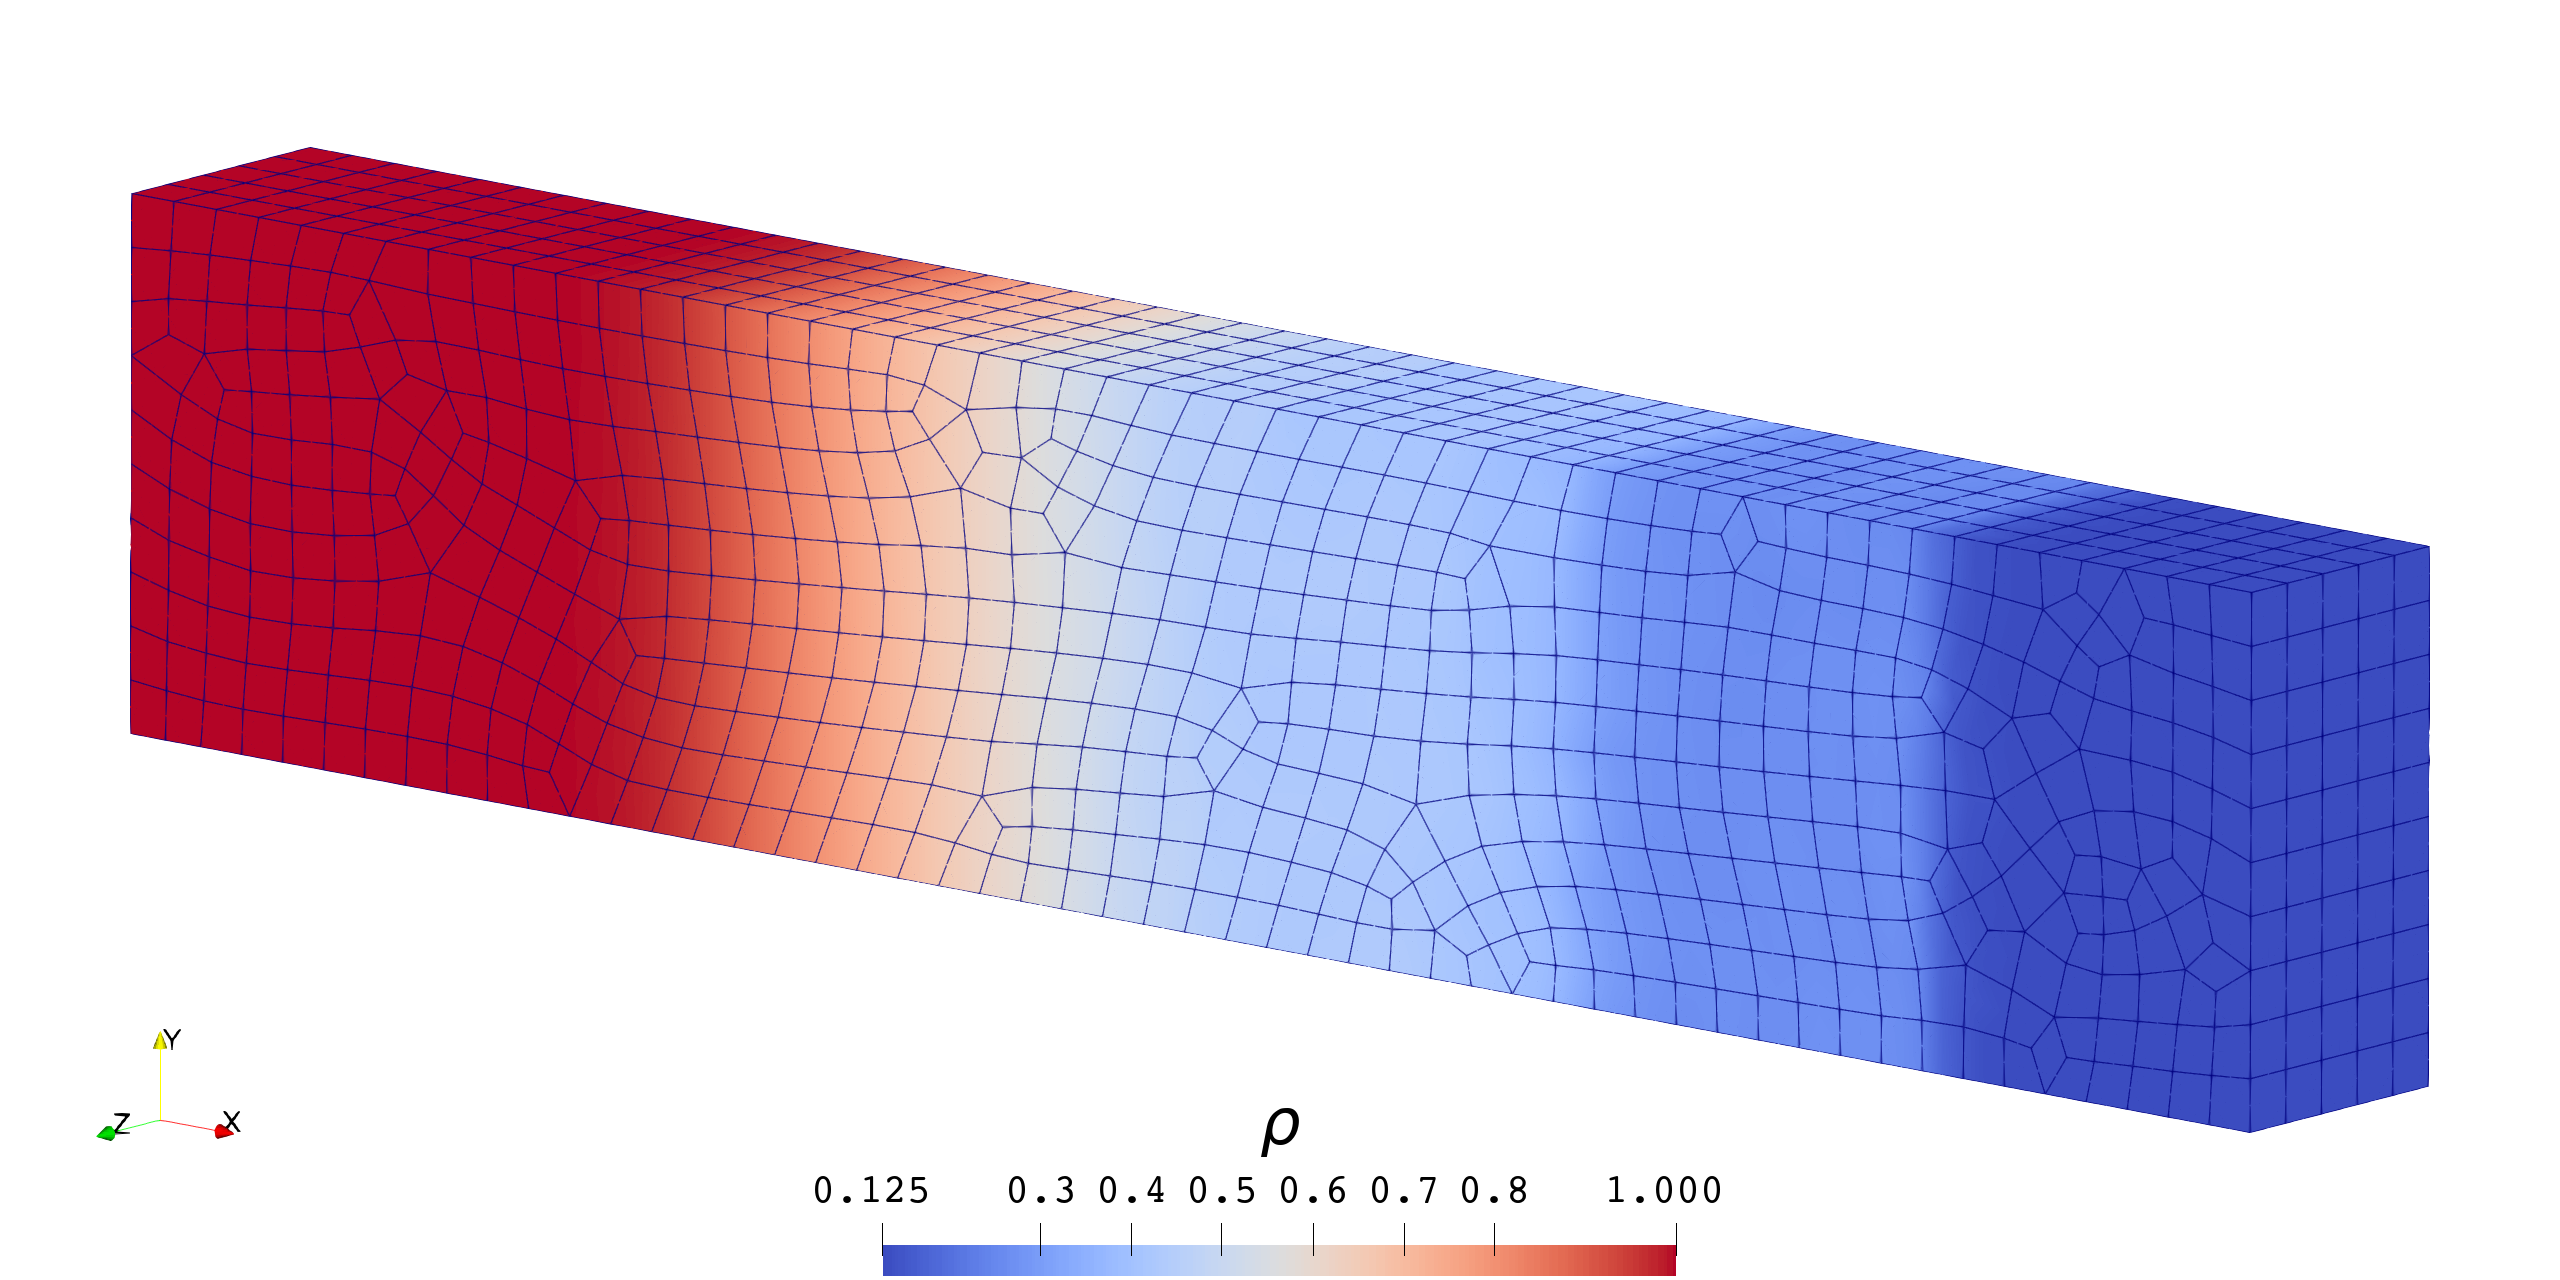
\includegraphics[width=0.98\textwidth]{figures/shock_tubes/sod/contour}

\caption{\label{fig:sod_contour}{Third-order} solution of $\rho(t=1.0)$ in
Problem \ref{prob:sod}.}
\end{figure}
\vspace{-12pt}

\begin{figure}[H]
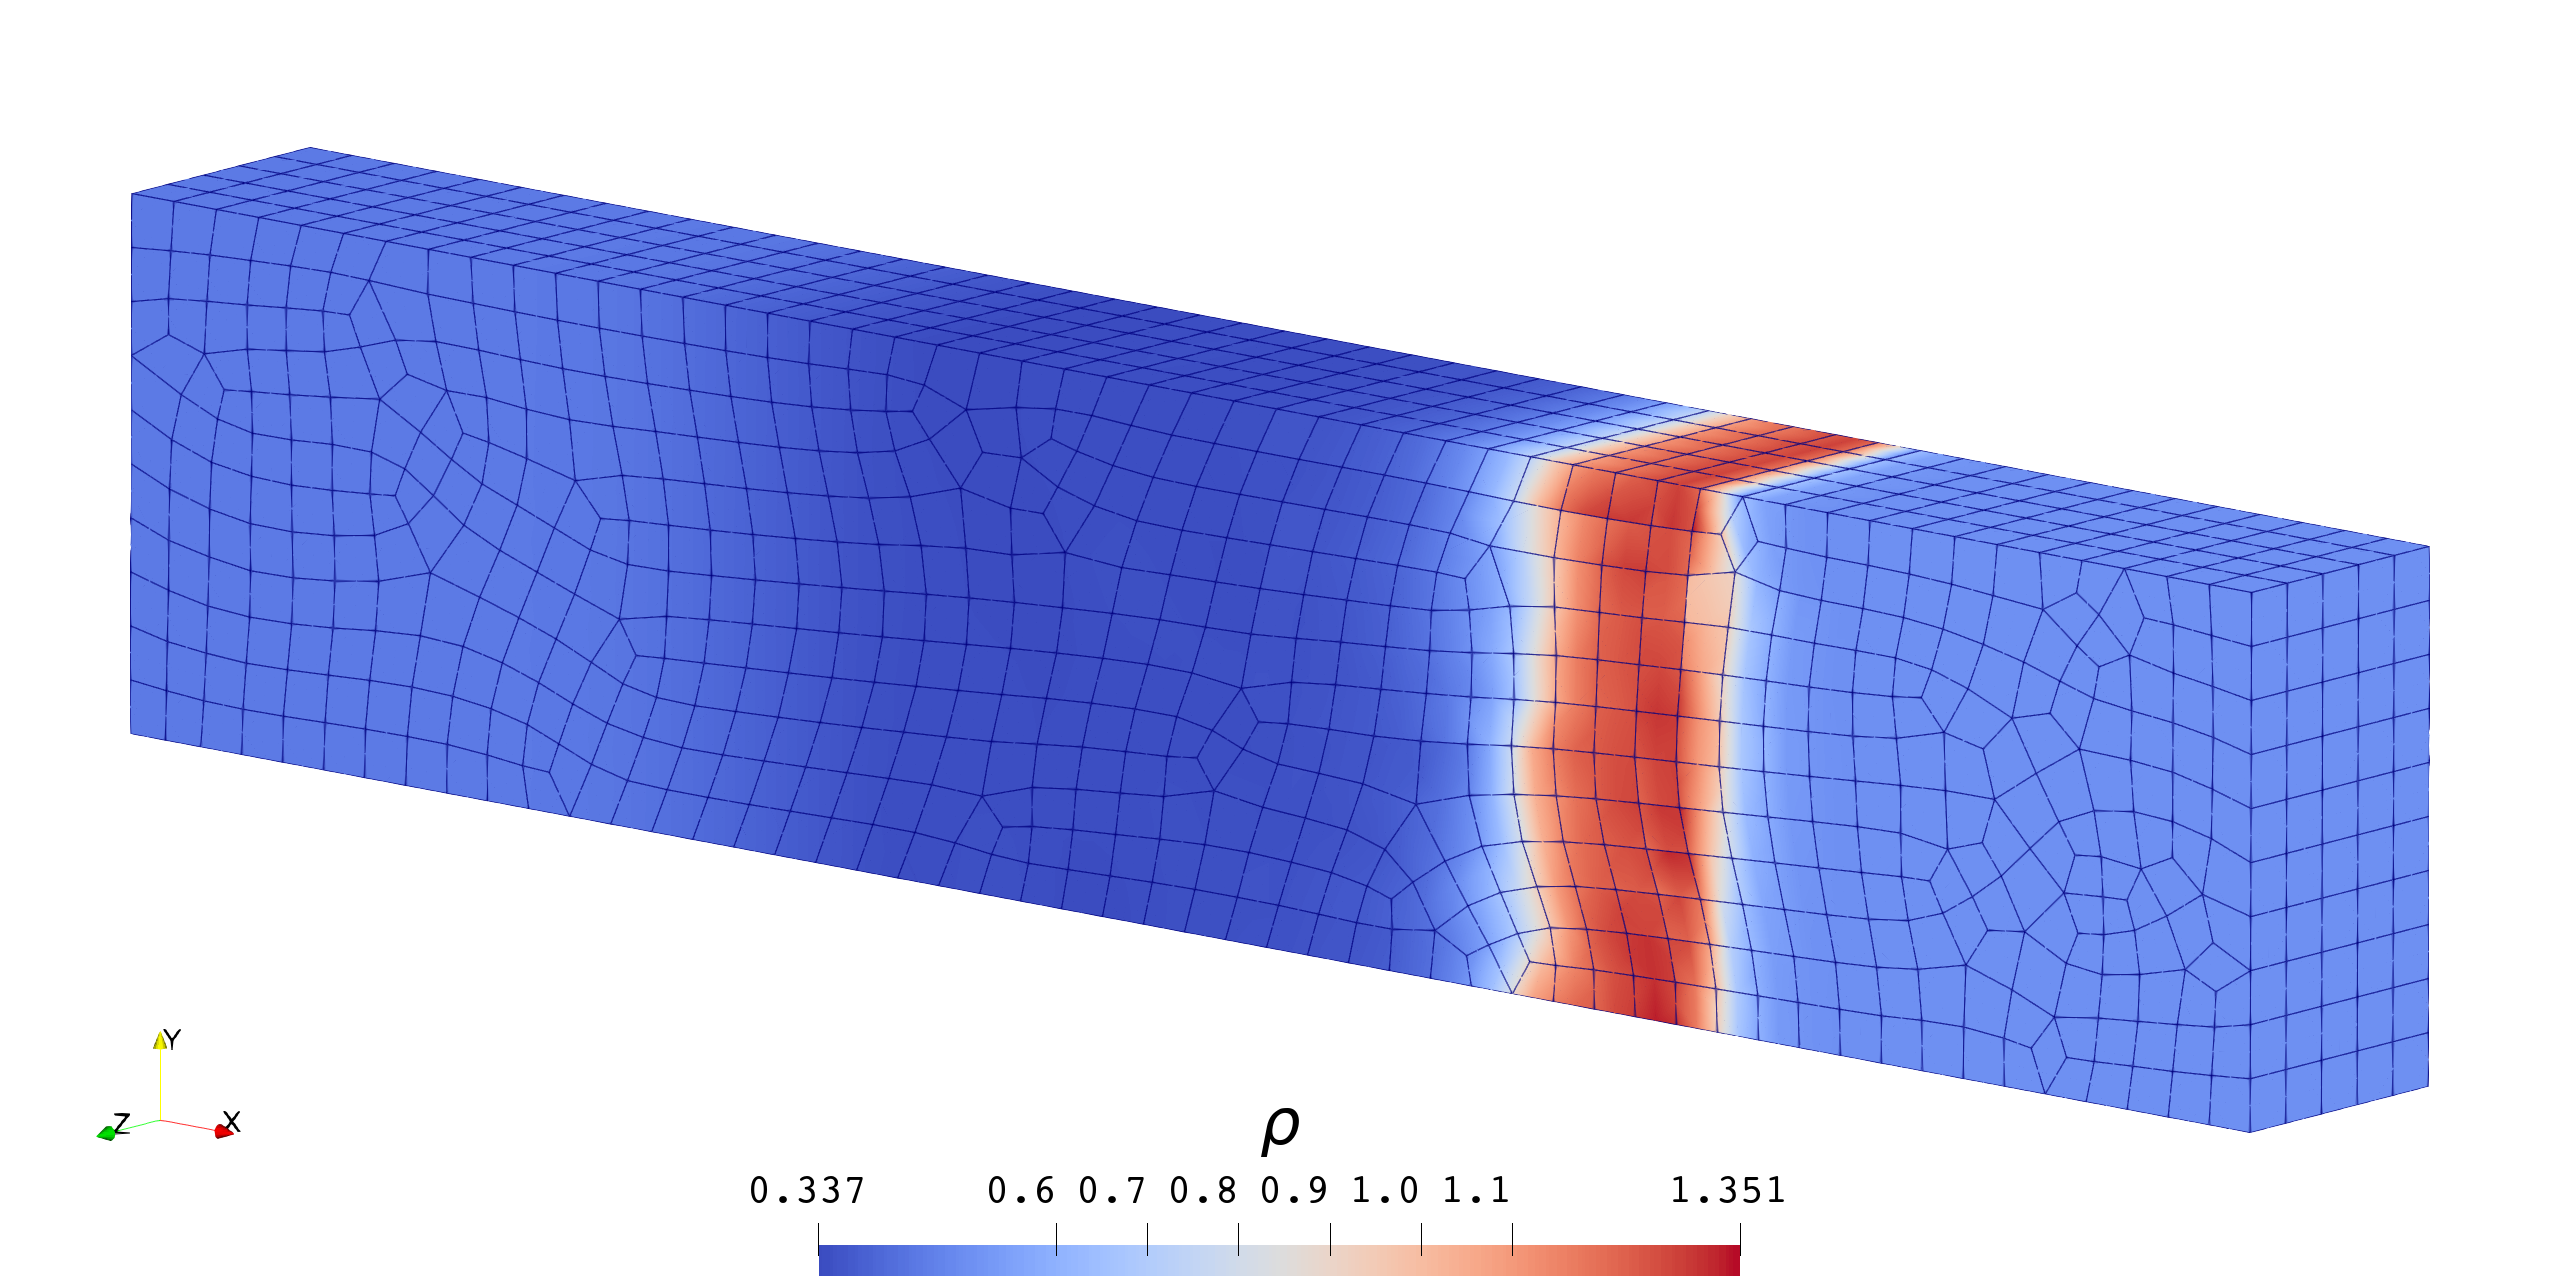
\includegraphics[width=0.99\textwidth]{figures/shock_tubes/lax/contour}

\caption{\label{fig:lax_contour}{Third-order} solution of $\rho(t=0.6)$ in
Problem \ref{prob:lax}.}
\end{figure}
\vspace{-12pt}

\begin{figure}[H]
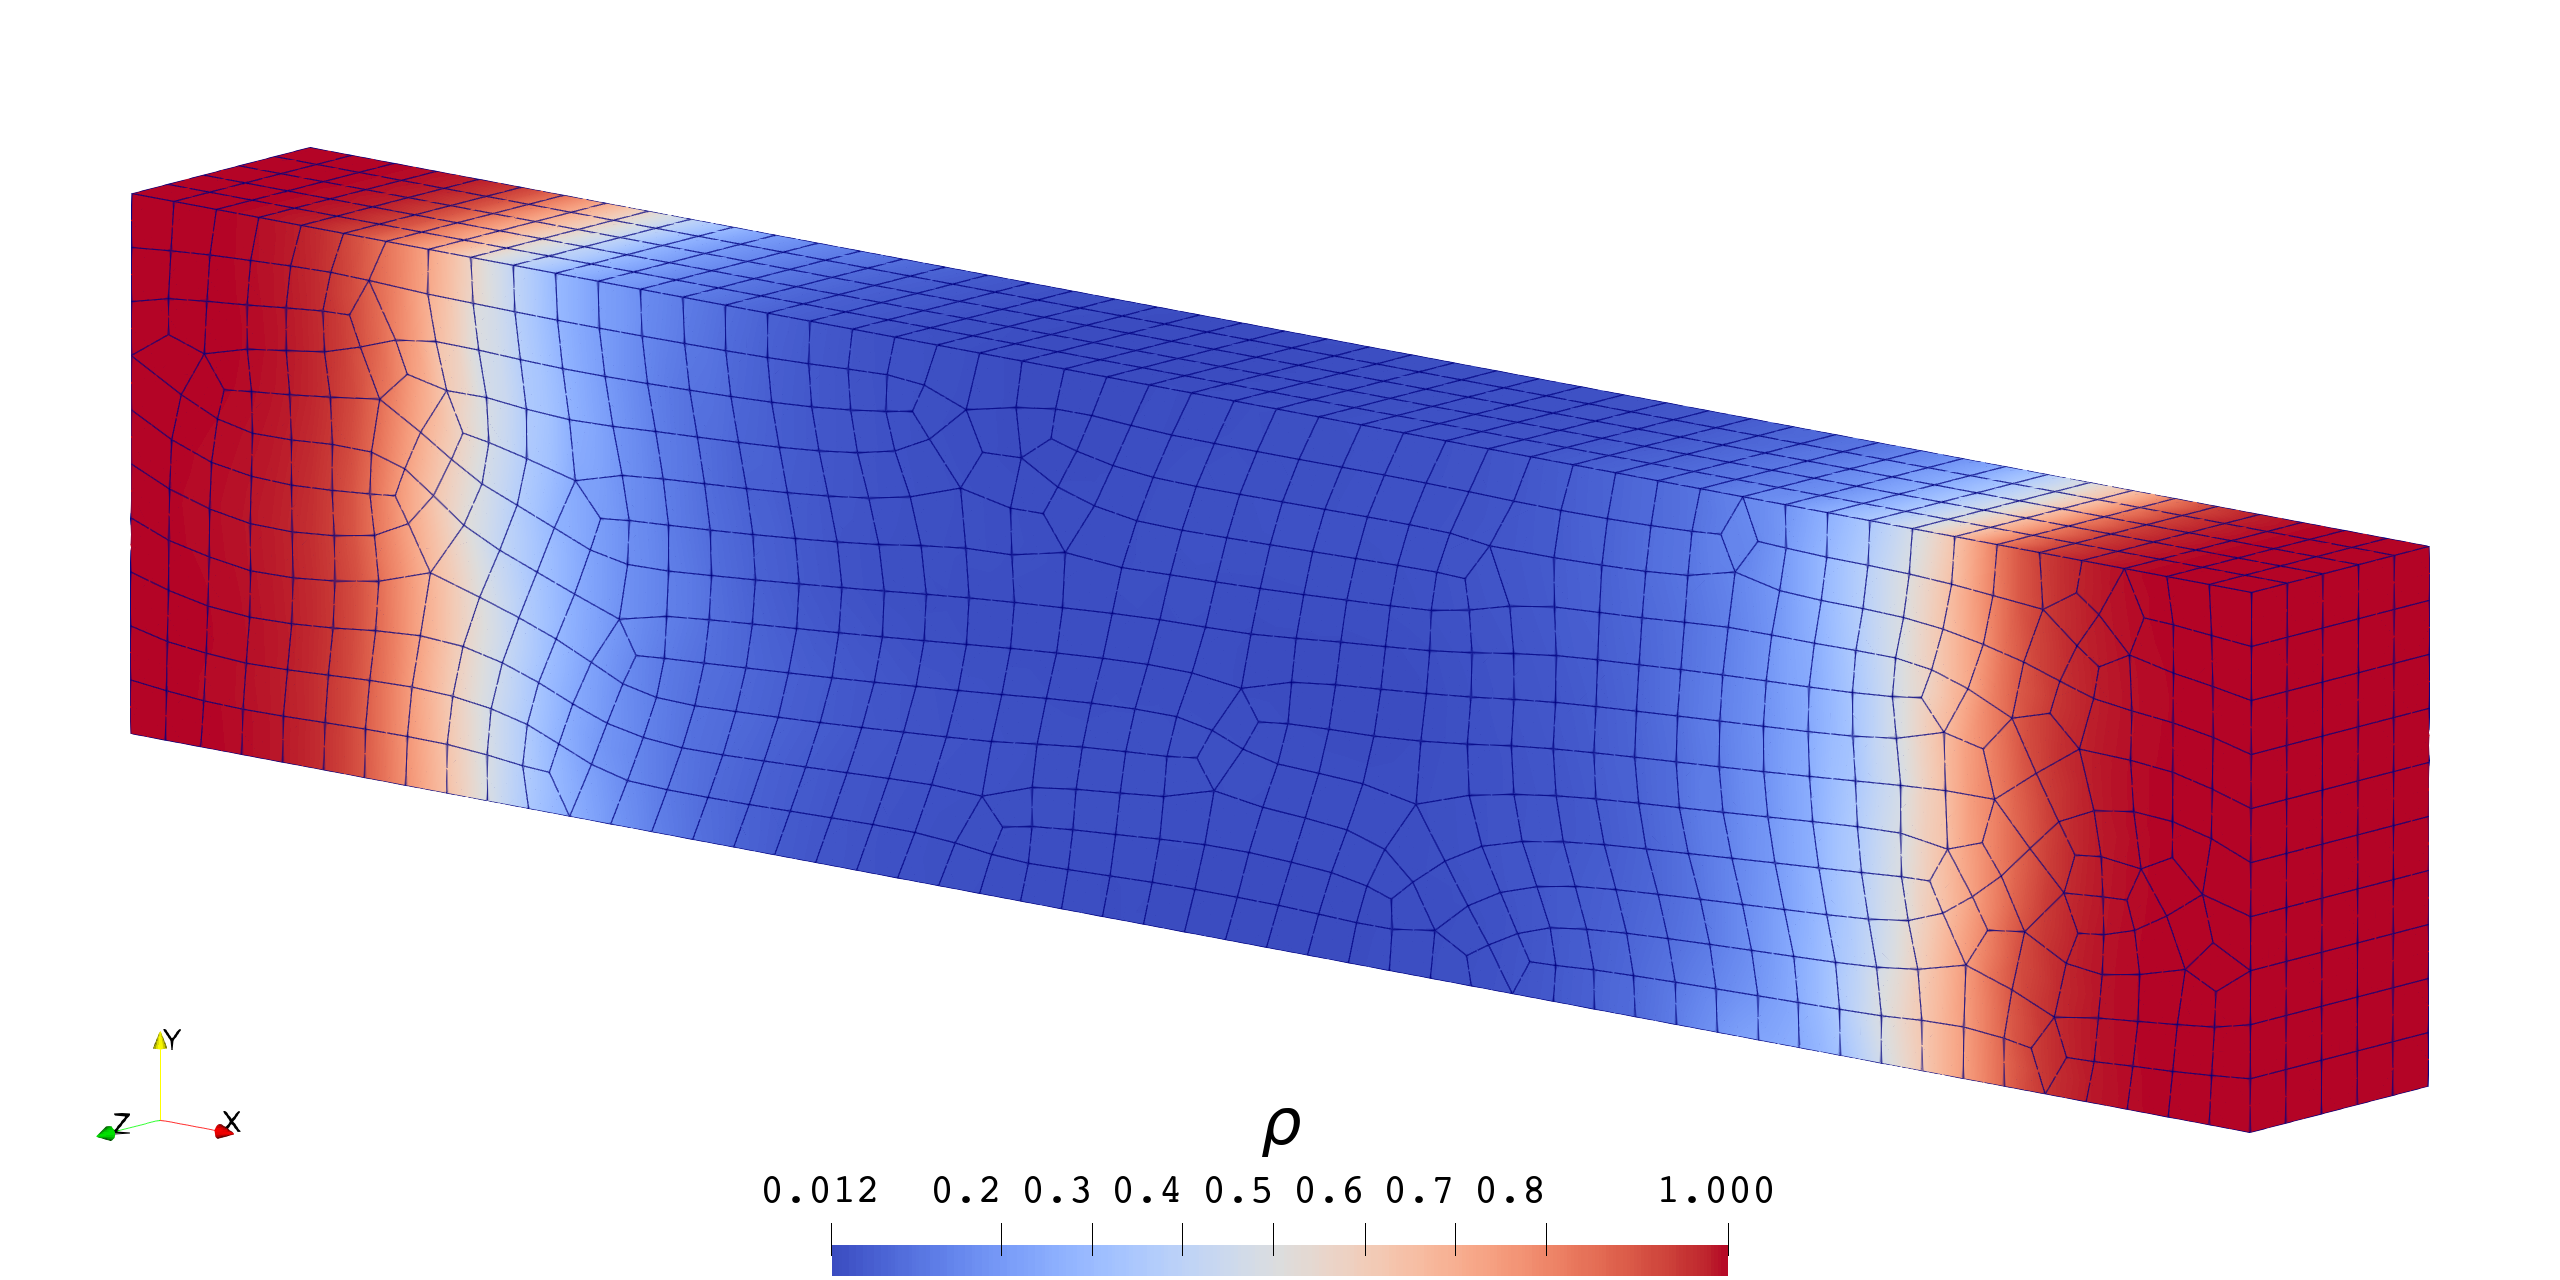
\includegraphics[width=0.98\textwidth]{figures/shock_tubes/vacuum/contour}

\caption{\label{fig:vacuum_contour}{Third-order} solution of $\rho(t=0.3)$
in Problem \ref{prob:vacuum}.}
\end{figure}
\vspace{-12pt}

\begin{figure}[H]
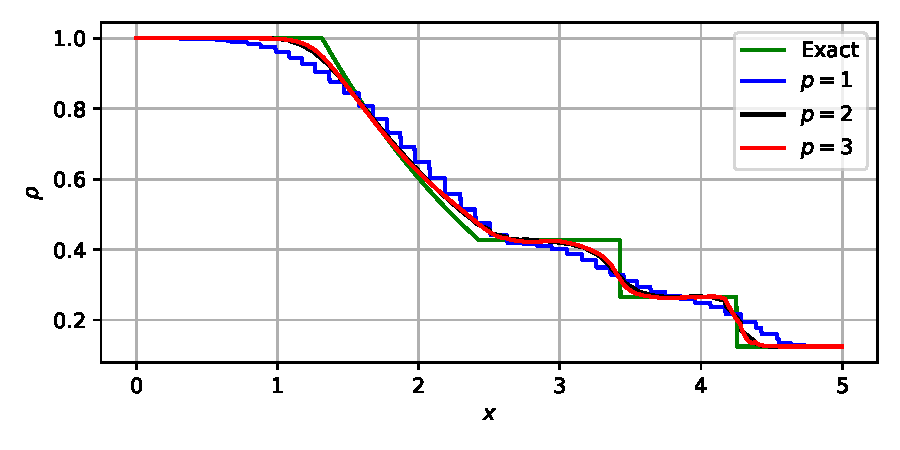
\includegraphics[width=0.99\textwidth]{figures/shock_tubes/sod/result}

\caption{\label{fig:sod}{Comparison between} solutions of $\rho(t=1.0)$ in
Problem \ref{prob:sod}.}
\end{figure}

\vspace{-12pt}
\begin{figure}[H]
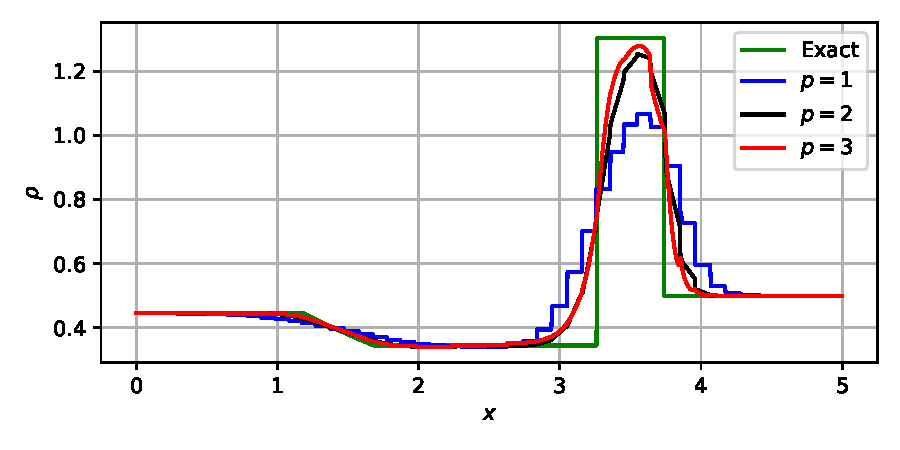
\includegraphics[width=0.99\textwidth]{figures/shock_tubes/lax/result}

\caption{\label{fig:lax}Comparison between solutions of $\rho(t=0.5)$ in
Problem \ref{prob:lax}.}
\end{figure}
\vspace{-12pt}

\begin{figure}[H]
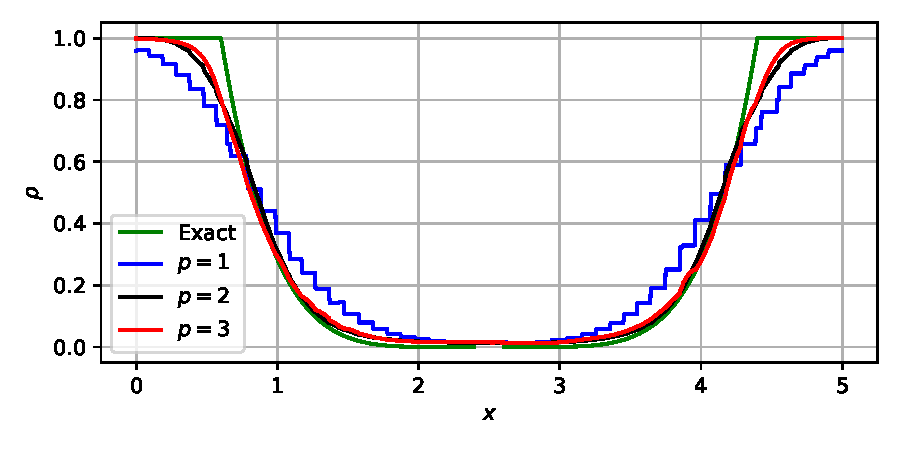
\includegraphics[width=0.99\textwidth]{figures/shock_tubes/vacuum/result}

\caption{\label{fig:vacuum}Comparison between solutions of $\rho(t=0.3)$
in Problem \ref{prob:vacuum}.}
\end{figure}


\subsubsection{Double Mach Reflection Problem}

This is a classical two-dimensional problem originally proposed in
\citep{Woodward_1984}, which we redefine here as a three-dimensional
one:
\begin{Problem}
\label{prob:double_mach}Solve the Euler system (Equation (\ref{eq:euler_system}))
in the region defined in Figure \ref{fig:double_mach_sketch}, in
which $x_{0}=1/6$. The initial condition is given as a moving shock wave:
\begin{equation}
\begin{bmatrix}\rho & u & vs. & w & p\end{bmatrix}_{t=0}=\begin{cases}
\begin{bmatrix}1.4 & 0.0 & 0.0 & 0.0 & 1.0\end{bmatrix} & y<\sqrt{3}(x-x_{0})\vspace{2pt}\\
\begin{bmatrix}8.0 & u_{\mathrm{A}} & v_{\mathrm{A}} & 0.0 & 116.5\end{bmatrix} & y>\sqrt{3}(x-x_{0})
\end{cases},\label{eq:double_mach_ic}
\end{equation}
in which $u_{\mathrm{A}}=4.125\sqrt{3}$ and $v_{\mathrm{A}}=-4.125$
are the velocity components \uline{a}fter the shock wave. The boundary
conditions are given as following:
\begin{itemize}
\item The $x=0$ surface is open as an inlet;
\item The $x=4$ surface and the $x<x_{0}$ part of the $y=0$ surface are
open as outlets;
\item The $x>x_{0}$ part of the $y=0$ surface is closed as a solid wall;
\item The $y=1$ surface has the following prescribed state:
\end{itemize}
\[
\begin{bmatrix}\rho & u & vs. & w & p\end{bmatrix}=\begin{cases}
\begin{bmatrix}1.4 & 0.0 & 0.0 & 0.0 & 1.0\end{bmatrix} & 1<\sqrt{3}(x-(x_{0}+u_{\mathrm{A}}t))\vspace{2pt}\\
\begin{bmatrix}8.0 & u_{\mathrm{A}} & v_{\mathrm{A}} & 0.0 & 116.5\end{bmatrix} & 1>\sqrt{3}(x-(x_{0}+u_{\mathrm{A}}t))
\end{cases},
\]
which is consistent with the initial condition (Equation (\ref{eq:double_mach_ic})).
\end{Problem}

As a common practice, we plot the density contour at $t=0.2$ in a
$[0,3]\times[0,1]$ rectangle (on the $z=0$ surface) for each solver
in Figures \ref{fig:double_mach_p=00003D1_h=00003D5e-3}--\ref{fig:double_mach_p=00003D3_h=00003D5e-3}.
It is clear that as the accuracy order increases, the thickness of
each discontinuity decreases and the rolled-up vortex structure becomes
more clear.

Before concluding this section, we provide the measured performance of our
third-order solver that produces Figure \ref{fig:double_mach_p=00003D3_h=00003D5e-3}
in Table \ref{tab:parallel_efficiency}, in which
\begin{itemize}
\item $P$ means the number of processes (one process per core).
\item $T_{n}$ means the wall clock time to finish the first $n$ step.
\item $P\frac{T_{m+m}-T_{n}}{m}$ is the core time per step. The total core
time of all steps is often used as an index for charging by high performance
computing centers.
\end{itemize}

\begin{figure}[H]
\begin{tikzpicture}[scale=3, rotate=30]
% axes
\draw[->] (4,0) -- +(0.2,0) node[below] {$x$};
\draw[->] (0,1) -- +(0,.2) node[above] {$y$};
% ticks
\foreach \i in {0,...,4}
  \draw (\i,0) -- +(0,-.05) node[below] {$\i$};
\foreach \i in {0,1}
  \draw (0,\i) -- +(-.04,0) node[left] {$\i$};
% lines and nodes
\draw[ultra thick, red!80!black] (0.25,0) coordinate (x0) -- +(60:3) coordinate (us);
\draw[ultra thick, red!80!black] (x0) -- +(-120:0.5) coordinate (ut);
\draw[dashed] (0,0) rectangle (4,1);
\path (us) -- (x0 -| us) coordinate (xs);
\draw[->] (us) -- +(-30:.3) node[right] {$u_\perp=8.25$};
\draw[->] (ut) -- +(-30:.3) node[right] {$u_\perp=8.25$};
\draw[thick] (4,0) -- (x0) -- +(-60:.5) coordinate (xt);
\path node[left] at (x0) {$x_0$};
% angle
\draw pic[draw,pic text=$\pi/3$, angle eccentricity=1.8, angle radius=.6cm] {angle=xs--x0--us};
\draw pic[draw,pic text=$\pi/3$, angle eccentricity=2.0, angle radius=.6cm] {angle=xt--x0--xs};
\end{tikzpicture}

\caption{\label{fig:double_mach_sketch}A schematic diagram of Problem \ref{prob:double_mach}.
The rectangle bounded by four dashed lines and a solid line is the
computational domain. The thick red line represents the initial shock
wave, which is at an angle of $\pi/3$ relative to the $x$-axis.}
\end{figure}
\vspace{-12pt}



\begin{figure}[H]
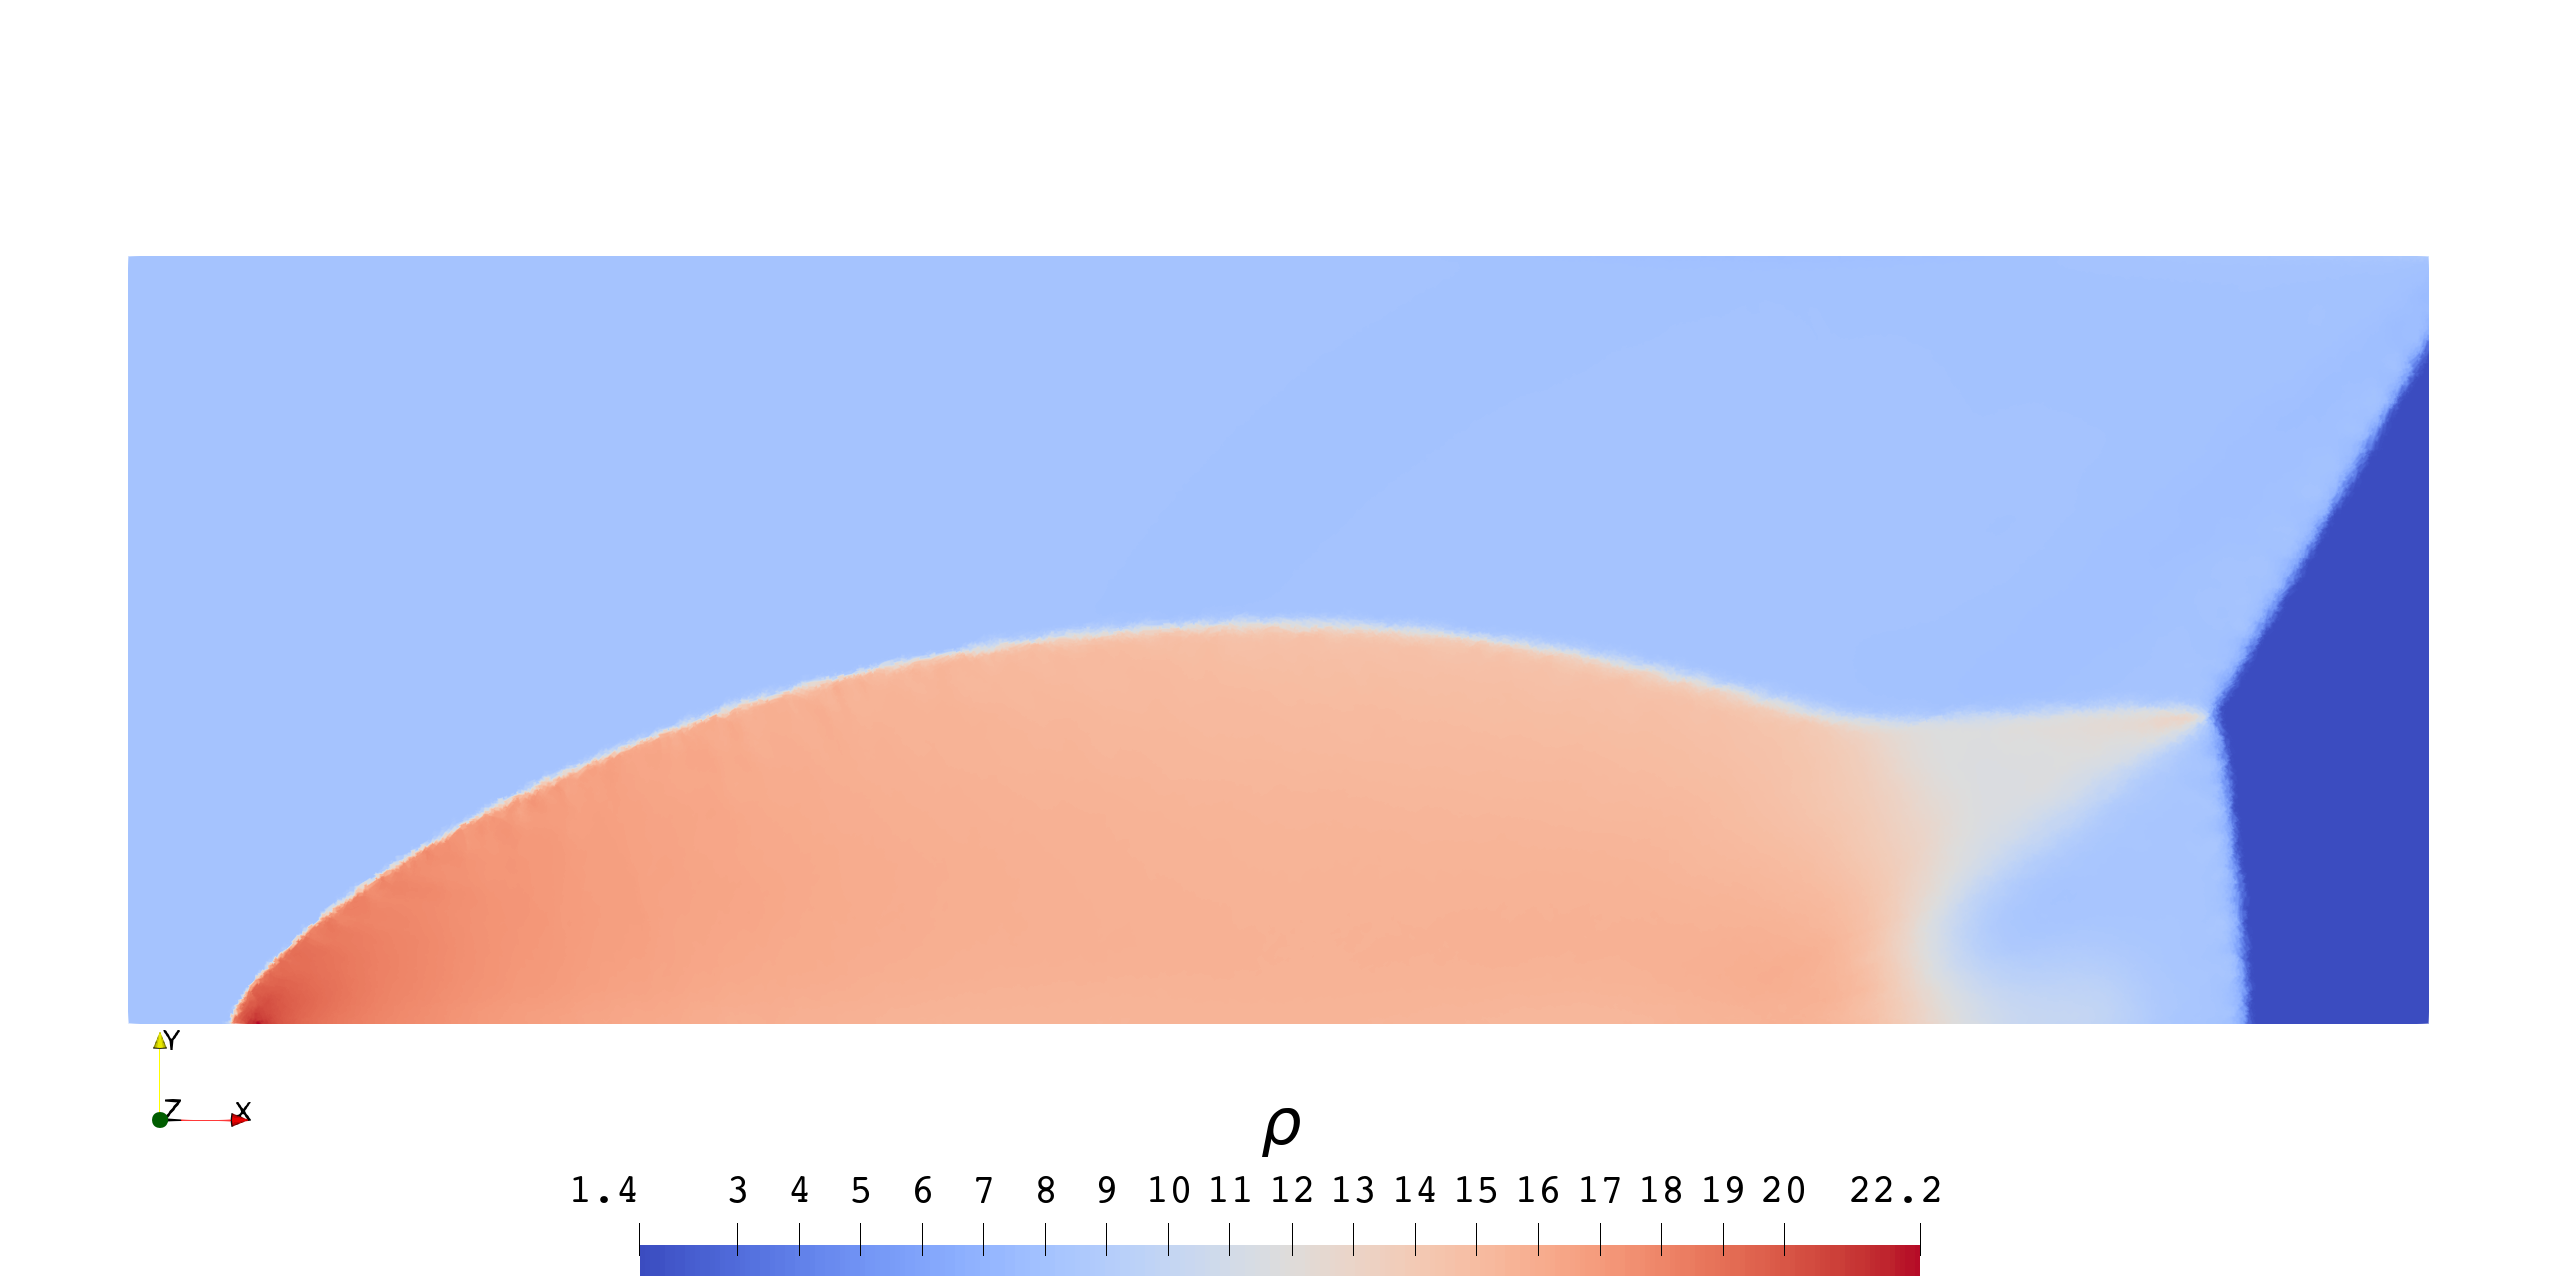
\includegraphics[width=0.99\textwidth]{figures/double_mach/p=1_h=5e-3}

\caption{\label{fig:double_mach_p=00003D1_h=00003D5e-3}{First-order solution}
of $\rho(x,y,z=0,t=0.2)$ in Problem \ref{prob:double_mach} ($h\approx1/200$).}
\end{figure}

Since parallel I/O operations require many collective communications,
we write one frame every 100 steps. Thus, the difference between the
values in the last two columns is the amortized core time of writing
per step. We have to admit that this cost is growing as the number
of cores increases. If the number of cores keeps increasing, this
may be a bottleneck of maintaining scalability.

The community of parallel computing usually use the speedup ($S$)
and efficiency ($E$) defined as
\[
S=\frac{T_{\text{serial}}}{T_{\text{parallel}}},\qquad E=\frac{S}{P}\times100\%,
\]
to assess the performance a parallel program. We follow this practice,
calculate these values based on the measured data given in Table \ref{tab:parallel_efficiency}
and plot them in Figures \ref{fig:double_mach_speedup} and \ref{fig:double_mach_efficiency}.
These figures show again that the I/O operations have adverse effects
on the parallel performance.

\begin{figure}[H]
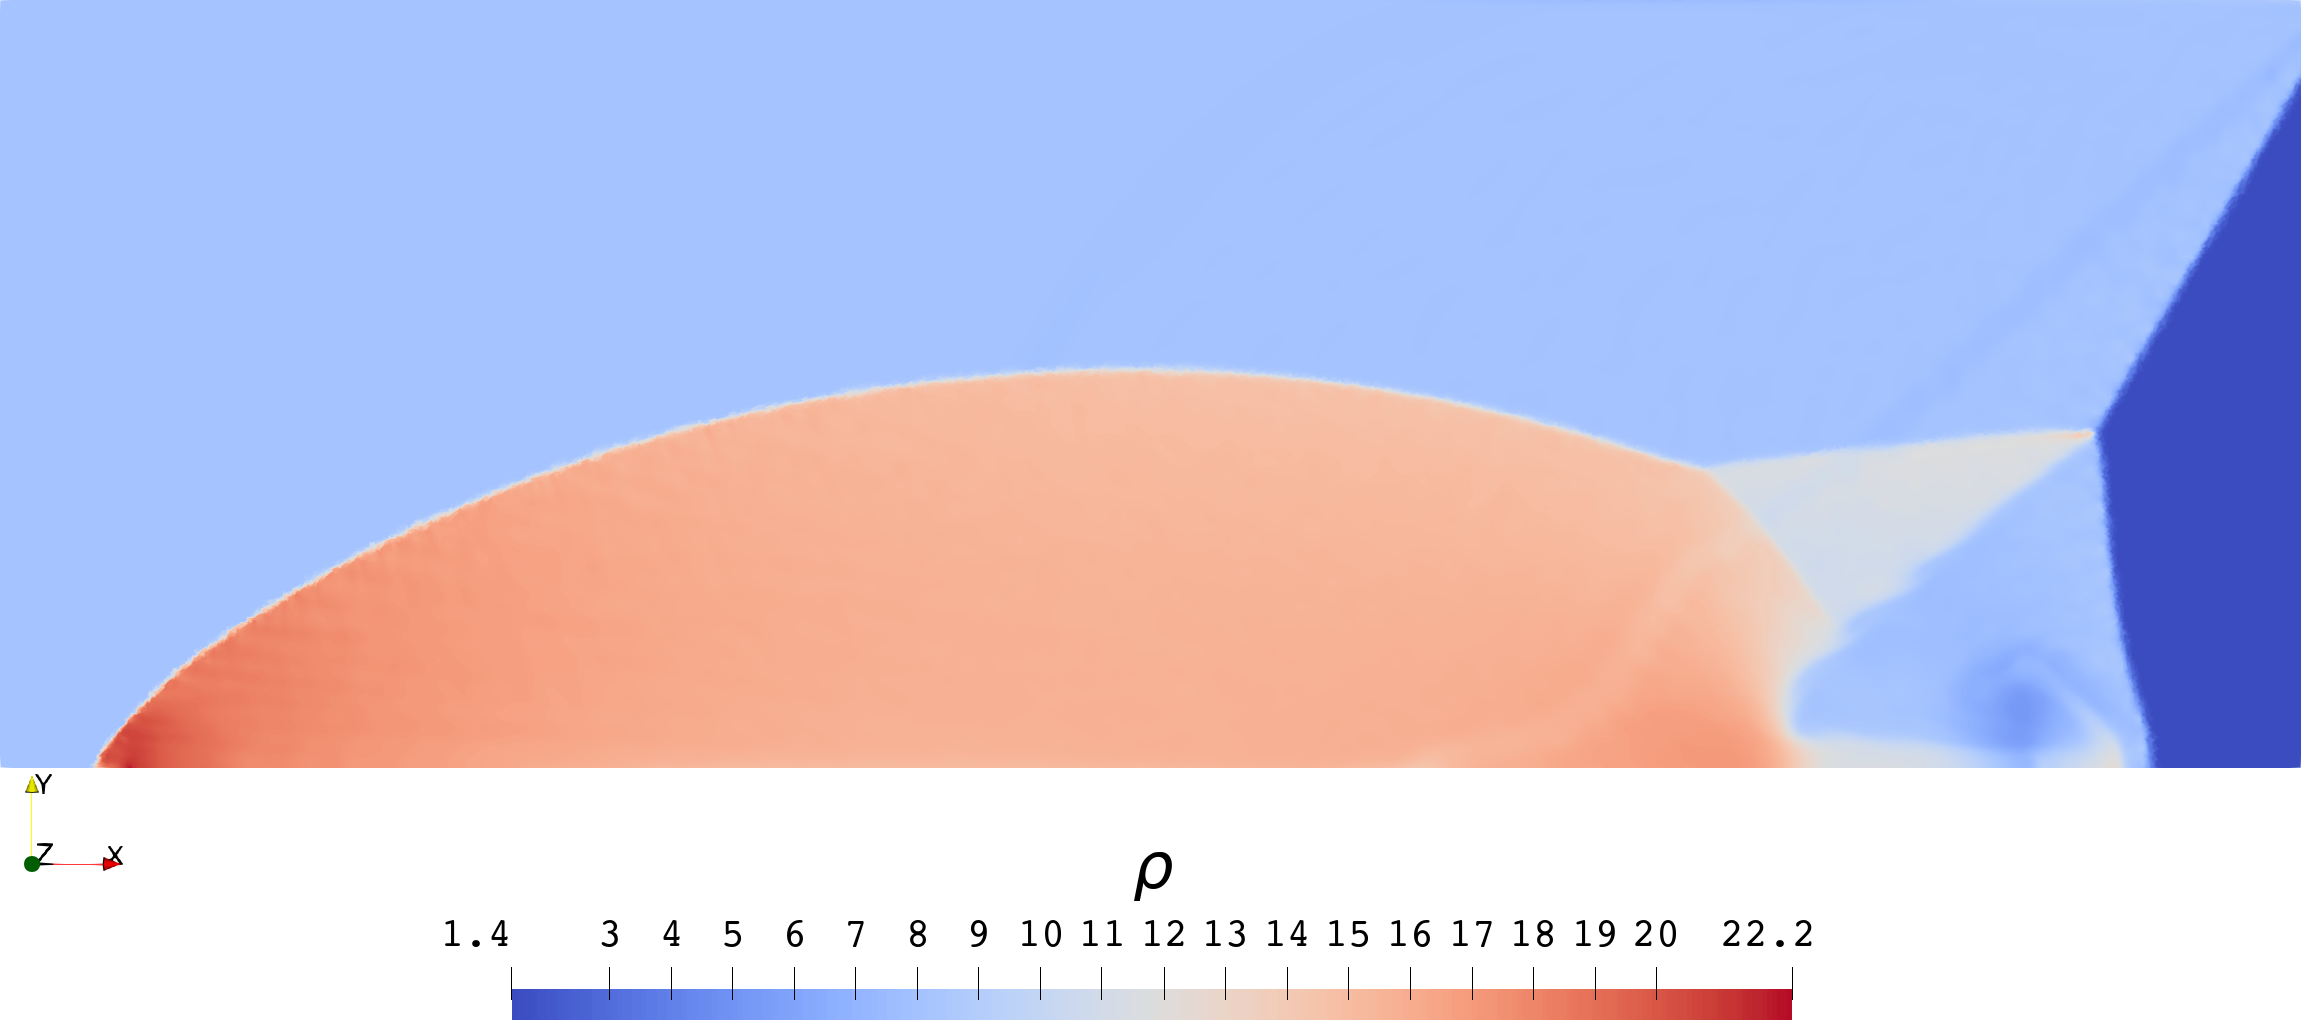
\includegraphics[width=0.99\textwidth]{figures/double_mach/p=2_h=5e-3}

\caption{\label{fig:double_mach_p=00003D2_h=00003D5e-3}{Second-order solution}
of $\rho(x,y,z=0,t=0.2)$ in Problem \ref{prob:double_mach} ($h\approx1/200$).}
\end{figure}
\vspace{-12pt}
\begin{figure}[H]
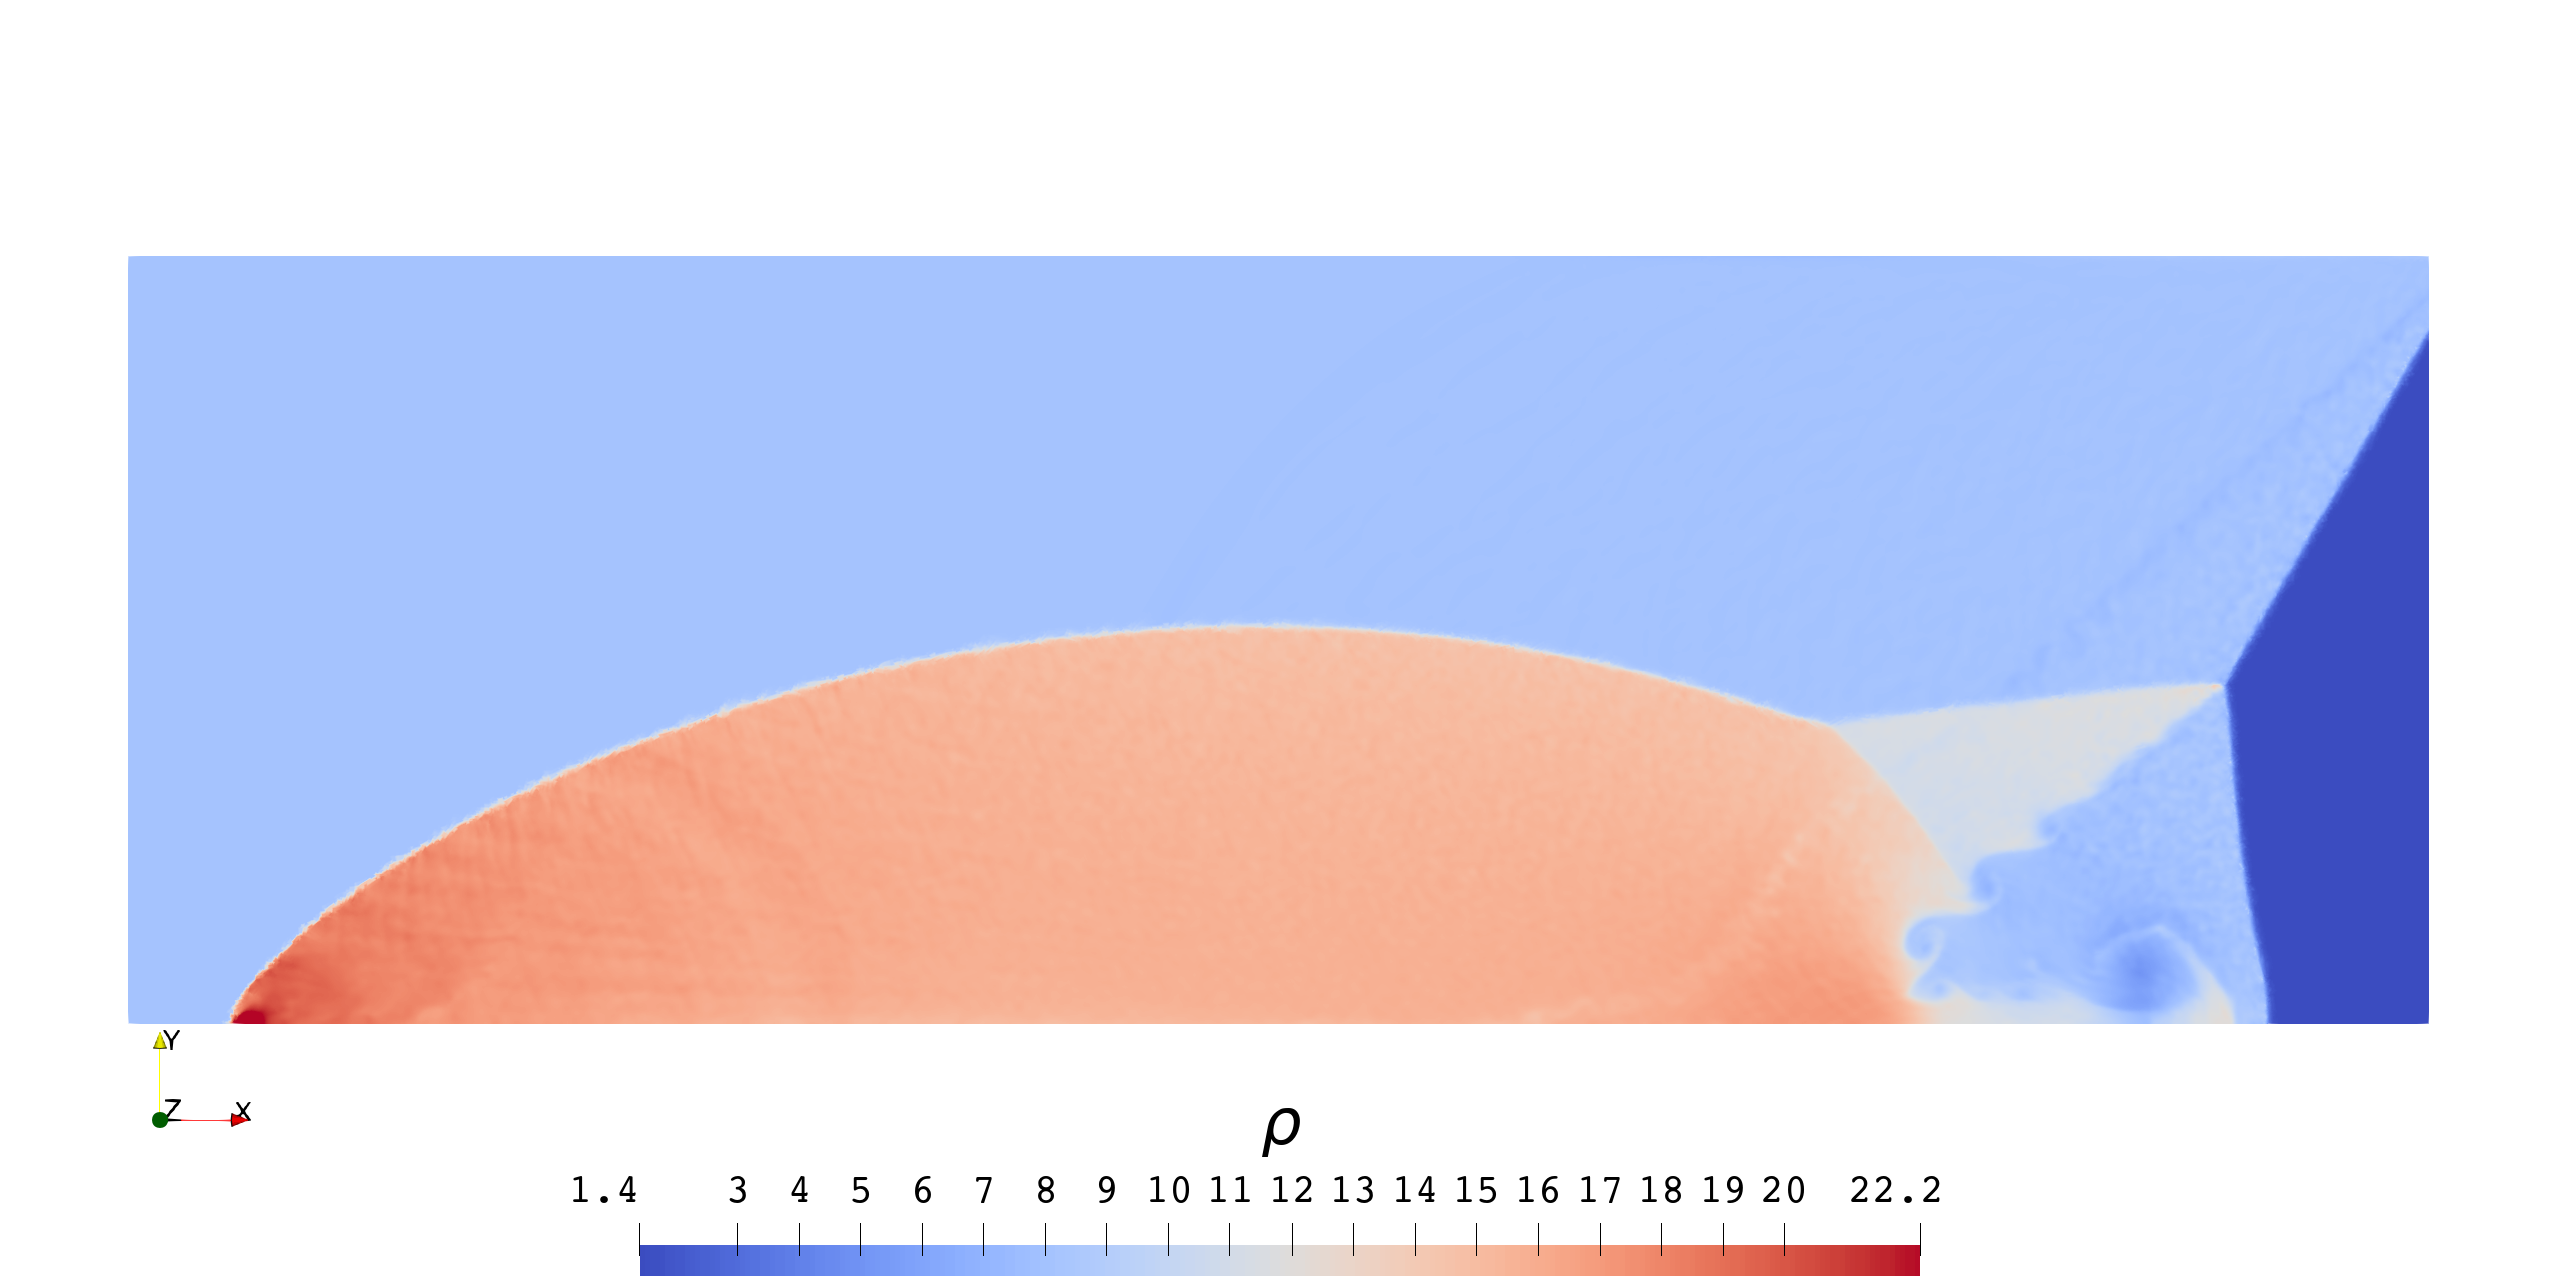
\includegraphics[width=0.99\textwidth]{figures/double_mach/p=3_h=5e-3}

\caption{\label{fig:double_mach_p=00003D3_h=00003D5e-3}{Third-order solution}
of $\rho(x,y,z=0,t=0.2)$ in Problem \ref{prob:double_mach} ($h\approx1/200$).}
\end{figure}
\unskip

%
\begin{table}[H]
\caption{\label{tab:parallel_efficiency}Performance of the same solver running
on different number of cores.}

\begin{tabular*}{1\textwidth}{@{\extracolsep{\fill}}>{\centering}p{0.1\textwidth}>{\centering}p{0.1\textwidth}>{\centering}p{0.1\textwidth}>{\centering}p{0.1\textwidth}>{\centering}p{0.1\textwidth}>{\centering}p{0.1\textwidth}}
\toprule 
\textbf{\boldmath{$P$}} & \textbf{\boldmath{$T_{100}$}} & \textbf{\boldmath{$T_{199}$}} & \textbf{\boldmath{$T_{200}$}} & \boldmath{$P\frac{T_{199}-T_{100}}{99}$} & \boldmath{$P\frac{T_{200}-T_{100}}{100}$}\tabularnewline
\midrule 
1 & 17,652.2 & 35,324.5 & 35,519.3 & 178.508 & 178.671\tabularnewline
20 & 960.443 & 1912.365 & 1926.584 & 192.307 & 193.228 \tabularnewline
40 & 491.070 & 971.710 & 983.933 & 194.198 & 197.145\tabularnewline
60 & 335.651 & 666.548 & 676.930 & 200.544 & 204.767\tabularnewline
80 & 251.548 & 494.541 & 504.951 & 196.358 & 202.722\tabularnewline
100 & 202.789 & 397.641 & 408.126 & 196.820 & 205.337\tabularnewline
\bottomrule
\end{tabular*}
\end{table}

The efficiency values given in Figure \ref{fig:double_mach_efficiency}
fluctuate around $90\%$, which are not as good as those above $99\%$
in \citep{Biswas_1994}. One source of such gap is the imperfect load
balancing of our tests. Since we are using a three-dimensional unstructured
mesh, it can hardly be partitioned uniformly, which is an $NP$-hard
problem. On the other hand, their meshes are one- and two-dimensional
structured, on which uniform partitioning can be trivially achieved.
\mbox{Figure \ref{fig:double_mach_balance}} gives the distribution of cells
of the 100-part mesh partitioning (\mbox{Figure \ref{fig:double_mach_partition}})
used in this section, which shows a $3\%$ fluctuation.



\begin{figure}[H]
\hspace{-1em}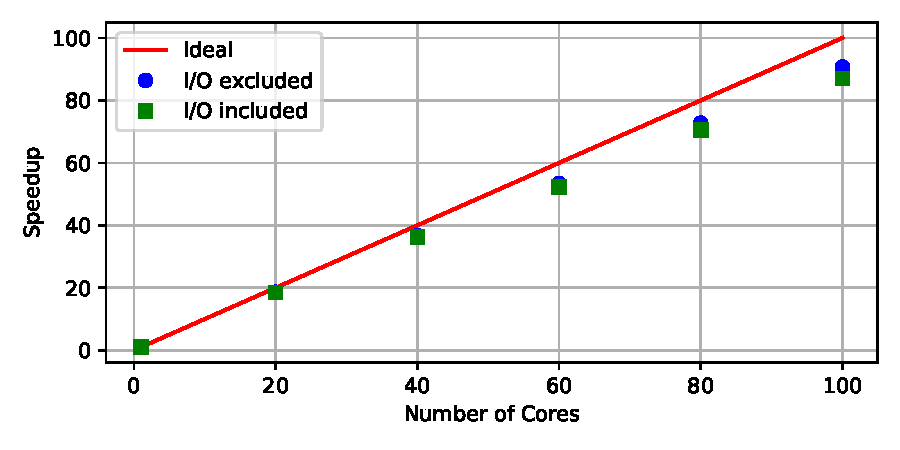
\includegraphics[width=0.99\textwidth]{figures/double_mach/speedup}

\caption{\label{fig:double_mach_speedup}Speedup of the third-order solver
for generating Figure \ref{fig:double_mach_p=00003D3_h=00003D5e-3}.}
\end{figure}
\vspace{-12pt}

\begin{figure}[H]
\hspace{-1em}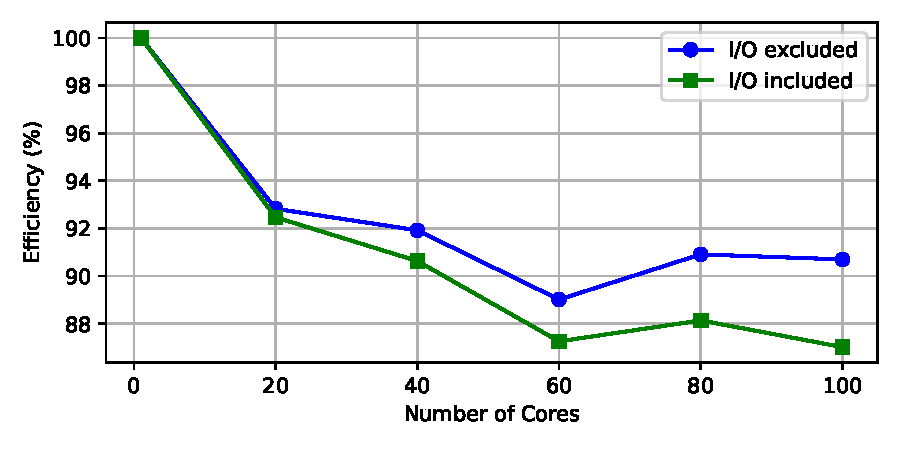
\includegraphics[width=0.99\textwidth]{figures/double_mach/efficiency}

\caption{\label{fig:double_mach_efficiency}Parallel efficiency of the third-order
solver for generating Figure \ref{fig:double_mach_p=00003D3_h=00003D5e-3}.}
\end{figure}
\unskip


\begin{figure}[H]
\hspace{-1em}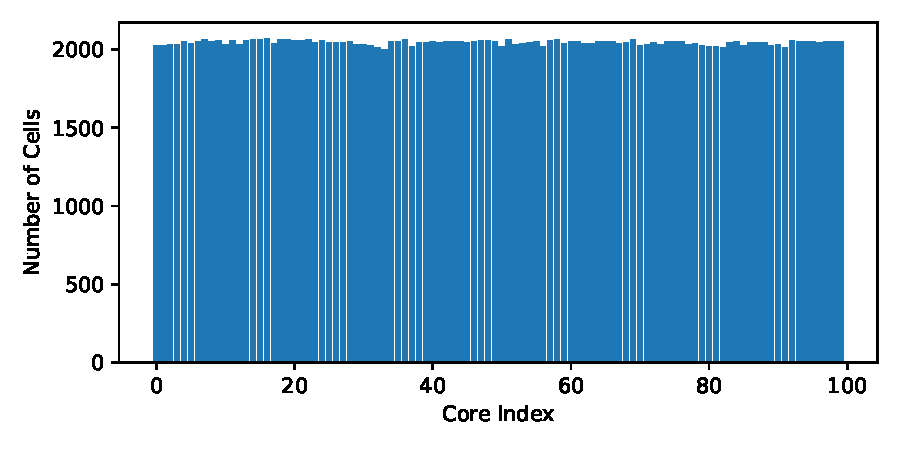
\includegraphics[width=0.99\textwidth]{figures/double_mach/balance}

\caption{\label{fig:double_mach_balance}Distribution of cells in the mesh
partitioning given in Figure \ref{fig:double_mach_partition}.}
\end{figure}
\vspace{-12pt}
\begin{figure}[H]
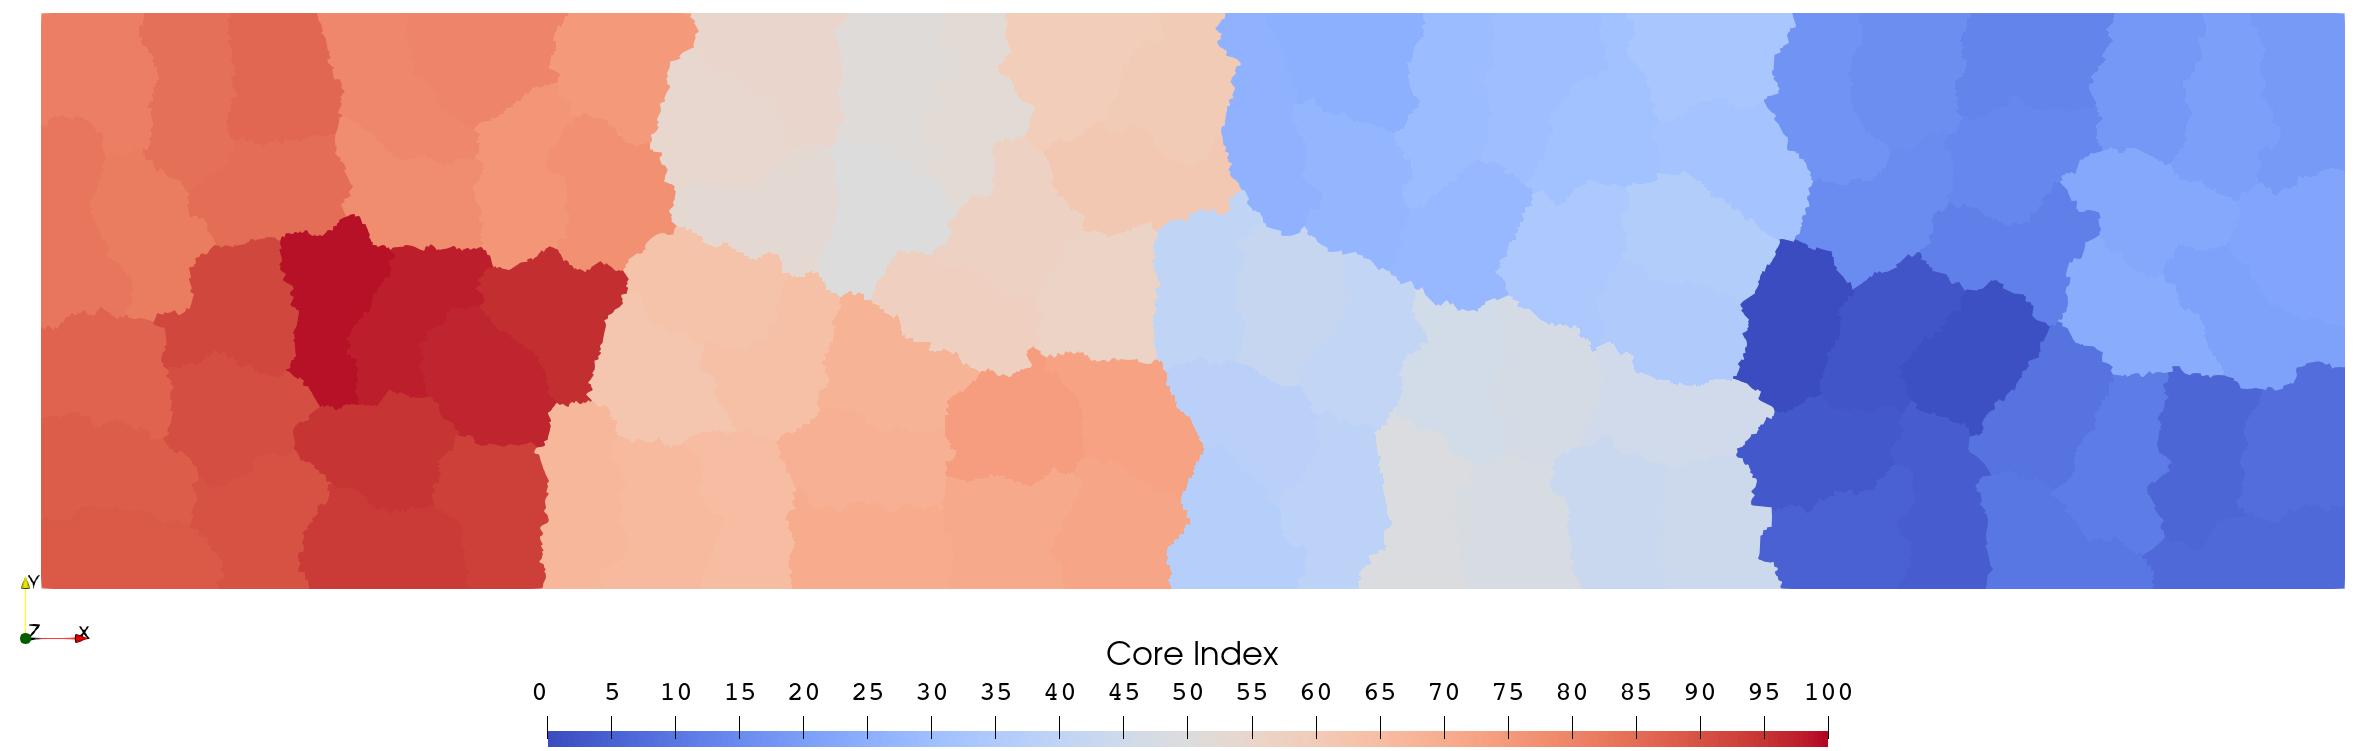
\includegraphics[width=0.99\textwidth]{figures/double_mach/partition}

\caption{\label{fig:double_mach_partition}{A 100-part mesh} partitioning of
the unstructured mesh used for generating Figures \ref{fig:double_mach_p=00003D1_h=00003D5e-3}--\ref{fig:double_mach_p=00003D3_h=00003D5e-3}.}
\end{figure}


\section{Discussion}

In this article, we have formulated the RKDG methods and the WENO
limiters for three-dimensional unstructured meshes. The algorithms
have been implemented on top of the MPI standard, which supports distributed
memory parallelization. The numerical experiments have shown that
increasing a solver's accuracy order helps more to produce better
results than just refining the mesh it uses. The efficient parallel
implementation has made the time cost affordable for large problems,
as long as the solvers can be executed on sufficiently large number
of cores. Extending the methods to Navier--Stokes equations and applications
of these high-order parallel solvers to real engineering problems
are ongoing works. Further optimization of the parallel I/O module
may be conducted to achieve better parallel performance.

\vspace{6pt}


\authorcontributions{Conceptualization, W.P. and S.L.; methodology, W.P.; software, W.P. and
Y.J.; validation, W.P. and Y.J.; formal analysis, W.P. and Y.J.;
investigation, W.P.; resources, W.P.; data curation, W.P.; writing---original
draft preparation, W.P.; writing---review and editing, W.P., Y.J.
and S.L.; visualization, W.P.; supervision, S.L.%please confirm  // Correct.
; project administration,
S.L.; funding acquisition, S.L. All authors have read and agreed to the
published version of the manuscript.}

\funding{This research was funded by the National High-tech R\&D Program of
China (863 Program) grant number 2012AA112201.}
\institutionalreview{{Not applicable.}}%In this section, you should add the Institutional Review Board Statement and approval number, if relevant to your study. You might choose to exclude this statement if the study did not require ethical approval. Please note that the Editorial Office might ask you for further information. Please add “The study was conducted in accordance with the Declaration of Helsinki, and approved by the Institutional Review Board (or Ethics Committee) of NAME OF INSTITUTE (protocol code XXX and date of approval).” for studies involving humans. OR “The animal study protocol was approved by the Institutional Review Board (or Ethics Committee) of NAME OF INSTITUTE (protocol code XXX and date of approval).” for studies involving animals. OR “Ethical review and approval were waived for this study due to REASON (please provide a detailed justification).” OR “Not applicable” for studies not involving humans or animals.
%MDPI: please add this part

\informedconsent{{Not applicable.}}%Any research article describing a study involving humans should contain this statement. Please add ``Informed consent was obtained from all subjects involved in the study.'' OR ``Patient consent was waived due to REASON (please provide a detailed justification).'' OR ``Not applicable'' for studies not involving humans. You might also choose to exclude this statement if the study did not involve humans. Written informed consent for publication must be obtained from participating patients who can be identified (including by the patients themselves). Please state ``Written informed consent has been obtained from the patient(s) to publish this paper'' if applicable.
\dataavailability{The data presented in this article are all generated from the source
code publicly {available in} our Git repository \url{https://github.com/pvc1989/miniCFD} accessed on 15~March 2022 (or the mirror site \url{https://gitee.com/pvc1989/miniCFD}, accessed on 15 March 2022).}

\acknowledgments{The authors would like to express the deepest appreciation to Zhou
Yukai for his professional assistance with typesetting and graphing.}

\conflictsofinterest{The authors declare no conflict of interest. The funders had no role
in the design of the study; in the collection, analyses, or interpretation
of data; in the writing of the manuscript; or in the decision to publish
the results.}

%\appendixtitles{no}

%\appendixstart{}

%\appendix

\begin{adjustwidth}{-\extralength}{0cm}


\reftitle{References}

\begin{thebibliography}{999}

\bibitem[Hesthaven and Warburton(2008)]{Hesthaven_2008}
Hesthaven, J.S.; Warburton, T.
\newblock {\em Nodal Discontinuous Galerkin Methods}; Springer: New York, NY, USA,  2008.
[\href{http://doi.org/10.1007/ 978-0-387-72067-8}{CrossRef}]


\bibitem[Reed and Hill(1973)]{Reed_1973}
Reed, W.H.; Hill, T.R.
\newblock \emph{Triangular Mesh Methods for the Neutron Transport Equation};
\newblock Technical Report LA-UR-73-479; Los Alamos Scientific Lab.: {Los Alamos, NM, USA,} 1973.

\bibitem[Chavent and Salzano(1982)]{Chavent_1982}
Chavent, G.; Salzano, G.
\newblock A finite-element method for the 1-D water flooding problem with
gravity.
\newblock {\em J. Comput. Phys.} {\bf 1982}, {\em
45},~307--344.
\newblock [\href{http://dx.doi.org/10.1016/0021-9991(82)90107-3}{CrossRef}]


\bibitem[Cockburn and Shu(1988)]{Cockburn_1988}
Cockburn, B.; Shu, C.W.
\newblock The Runge-Kutta local projection P1-discontinuous-Galerkin finite
element method for scalar conservation laws.
\newblock In Proceedings of the   1st National Fluid Dynamics Conference, Cincinnati, OH, USA, 25--28 July 1988; {American Institute of
Aeronautics and Astronautics:} Reston, VA, USA,
1988.
\newblock [\href{http://dx.doi.org/10.2514/6.1988-3797}{CrossRef}]


\bibitem[Shu and Osher(1988)]{Shu_1988}
Shu, C.W.; Osher, S.
\newblock Efficient implementation of essentially non-oscillatory
shock-capturing schemes.
\newblock {\em J. Comput. Phys.} {\bf 1988}, {\em
77},~439--471.
\newblock [\href{http://dx.doi.org/10.1016/0021-9991(88)90177-5}{CrossRef}]


\bibitem[Shu and Osher(1989)]{Shu_1989}
Shu, C.W.; Osher, S.
\newblock Efficient implementation of essentially non-oscillatory
shock-capturing schemes, {II}.
\newblock {\em J. Comput. Phys.} {\bf 1989}, {\em 83},~32--78.
\newblock [\href{http://dx.doi.org/10.1016/0021-9991(89)90222-2}{CrossRef}]


\bibitem[Cockburn \em{et~al.}(1989)Cockburn, Lin, and Shu]{Cockburn_1989}
Cockburn, B.; Lin, S.Y.; Shu, C.W.
\newblock {TVB} Runge-Kutta local projection discontinuous Galerkin finite
element method for conservation laws {III}: One-dimensional systems.
\newblock {\em J. Comput. Phys.} {\bf 1989}, {\em 84},~90--113.
\newblock [\href{http://dx.doi.org/10.1016/0021-9991(89)90183-6}{CrossRef}]


\bibitem[Cockburn \em{et~al.}(1990)Cockburn, Hou, and Shu]{Cockburn_1990}
Cockburn, B.; Hou, S.; Shu, C.W.
\newblock The {Runge-Kutta} local projection discontinuous {Galerkin} finite
element method for conservation laws. {IV}. The multidimensional case.
\newblock {\em Math. Comput.} {\bf 1990}, {\em 54},~545--581.
\newblock [\href{http://dx.doi.org/10.1090/s0025-5718-1990-1010597-0}{CrossRef}]


\bibitem[Cockburn(1998)]{Cockburn_1998}
Cockburn, B.
\newblock An introduction to the {Discontinuous Galerkin} method for
convection-dominated problems. In {\em Lecture Notes in Mathematics};
Springer: Berlin/Heidelberg, Germany, 1998; pp. 150--268.
\newblock [\href{http://dx.doi.org/10.1007/bfb0096353}{CrossRef}]


\bibitem[Bassi and Rebay(1997)]{Bassi_1997}
Bassi, F.; Rebay, S.
\newblock A High-Order Accurate Discontinuous Finite Element Method for the
Numerical Solution of the Compressible Navier{\textendash}Stokes Equations.
\newblock {\em J. Comput. Phys.} {\bf 1997}, {\em
131},~267--279.
\newblock [\href{http://dx.doi.org/10.1006/jcph.1996.5572}{CrossRef}]


\bibitem[Cockburn and Shu(1998)]{Cockburn_1998b}
Cockburn, B.; Shu, C.W.
\newblock The Local Discontinuous Galerkin Method for Time-Dependent
Convection-Diffusion Systems.
\newblock {\em {SIAM} J. Numer. Anal.} {\bf 1998}, {\em
35},~2440--2463.
\newblock [\href{http://dx.doi.org/10.1137/S0036142997316712}{CrossRef}]


\bibitem[Cockburn and Shu(2001)]{Cockburn_2001}
Cockburn, B.; Shu, C.W.
\newblock {Runge–Kutta} Discontinuous {Galerkin} Methods for
Convection-Dominated Problems.
\newblock {\em J. Sci. Comput.} {\bf 2001}, {\em 16},~173--261.
\newblock [\href{http://dx.doi.org/10.1023/A:1012873910884}{CrossRef}]


\bibitem[Gottlieb and Shu(1997)]{Gottlieb_1997}
Gottlieb, D.; Shu, C.W.
\newblock On the Gibbs Phenomenon and Its Resolution.
\newblock {\em SIAM Rev.} {\bf 1997}, {\em 39},~644–668.
 [\href{http://dx.doi.org/10.1137/S0036144596301390}{CrossRef}]


\bibitem[Leer(1977{\natexlab{a}})]{Van_Leer_1977}
Leer, B.V.
\newblock Towards the ultimate conservative difference scheme {III}.
Upstream-centered finite-difference schemes for ideal compressible flow.
\newblock {\em J. Comput. Phys.} {\bf 1977}, {\em
23},~263--275.
\newblock [\href{http://dx.doi.org/10.1016/0021-9991(77)90094-8}{CrossRef}]


\bibitem[Leer(1977{\natexlab{b}})]{Van_Leer_1977a}
Leer, B.V.
\newblock Towards the ultimate conservative difference scheme. {IV}. A new
approach to numerical convection.
\newblock {\em J. Comput. Phys.} {\bf 1977}, {\em
23},~276--299.
\newblock [\href{http://dx.doi.org/10.1016/0021-9991(77)90095-X}{CrossRef}]


\bibitem[van Leer(1979)]{van_Leer_1979}
van Leer, B.
\newblock Towards the ultimate conservative difference scheme. V. A
second-order sequel to Godunov{\textquotesingle}s method.
\newblock {\em J. Comput. Phys.} {\bf 1979}, {\em
32},~101--136.
\newblock [\href{http://dx.doi.org/10.1016/0021-9991(79)90145-1}{CrossRef}]


\bibitem[van Leer and Nishikawa(2021)]{van_Leer_2021}
van Leer, B.; Nishikawa, H.
\newblock Towards the ultimate understanding of {MUSCL}: Pitfalls in achieving
third-order accuracy.
\newblock {\em J. Comput. Phys.} {\bf 2021}, {\em 446},~110640.
\newblock [\href{http://dx.doi.org/10.1016/j.jcp.2021.110640}{CrossRef}]


\bibitem[Harten \em{et~al.}(1997)Harten, Engquist, Osher, and
Chakravarthy]{Harten_1997}
Harten, A.; Engquist, B.; Osher, S.; Chakravarthy, S.R.
\newblock Uniformly High Order Accurate Essentially Non-oscillatory Schemes,
{III}.
\newblock {\em J. Comput. Phys.} {\bf 1997}, {\em 131},~3--47.
\newblock [\href{http://dx.doi.org/10.1006/jcph.1996.5632}{CrossRef}]


\bibitem[Jiang and Shu(1996)]{Jiang_1996}
Jiang, G.S.; Shu, C.W.
\newblock Efficient Implementation of Weighted {ENO} Schemes.
\newblock {\em J. Comput. Phys.} {\bf 1996}, {\em
126},~202--228.
\newblock [\href{http://dx.doi.org/10.1006/jcph.1996.0130}{CrossRef}]


\bibitem[Hu and Shu(1999)]{Hu_1999}
Hu, C.; Shu, C.W.
\newblock Weighted Essentially Non-oscillatory Schemes on Triangular Meshes.
\newblock {\em J. Comput. Phys.} {\bf 1999}, {\em
150},~97--127.
\newblock [\href{http://dx.doi.org/10.1006/jcph.1998.6165}{CrossRef}]


\bibitem[Qiu and Shu(2005)]{Qiu_2005}
Qiu, J.; Shu, C.W.
\newblock Runge--Kutta Discontinuous Galerkin Method Using {WENO} Limiters.
\newblock {\em {SIAM} J. Sci. Comput.} {\bf 2005}, {\em
26},~907--929.
\newblock [\href{http://dx.doi.org/10.1137/S1064827503425298}{CrossRef}]


\bibitem[Zhu \em{et~al.}(2008)Zhu, Qiu, Shu, and Dumbser]{Zhu_2008}
Zhu, J.; Qiu, J.; Shu, C.W.; Dumbser, M.
\newblock Runge{\textendash}Kutta discontinuous Galerkin method using {WENO}
limiters {II}: Unstructured meshes.
\newblock {\em J. Comput. Phys.} {\bf 2008}, {\em
227},~4330--4353.
\newblock [\href{http://dx.doi.org/10.1016/j.jcp.2007.12.024}{CrossRef}]


\bibitem[Zhong and Shu(2013)]{Zhong_2013}
Zhong, X.; Shu, C.W.
\newblock A simple weighted essentially nonoscillatory limiter for
{Runge}{\textendash}{Kutta} discontinuous {Galerkin} methods.
\newblock {\em J. Comput. Phys.} {\bf 2013}, {\em
232},~397--415.
\newblock [\href{http://dx.doi.org/10.1016/j.jcp.2012.08.028}{CrossRef}]


\bibitem[Zhu \em{et~al.}(2013)Zhu, Zhong, Shu, and Qiu]{Zhu_2013}
Zhu, J.; Zhong, X.; Shu, C.W.; Qiu, J.
\newblock {Runge}{\textendash}{Kutta} discontinuous {Galerkin} method using a
new type of {WENO} limiters on unstructured meshes.
\newblock {\em J. Comput. Phys.} {\bf 2013}, {\em
248},~200--220.
\newblock [\href{http://dx.doi.org/10.1016/j.jcp.2013.04.012}{CrossRef}]


\bibitem[Mazaheri \em{et~al.}(2019)Mazaheri, Shu, and Perrier]{Mazaheri_2019}
Mazaheri, A.; Shu, C.W.; Perrier, V.
\newblock Bounded and compact weighted essentially nonoscillatory limiters for
discontinuous Galerkin schemes: Triangular elements.
\newblock {\em J. Comput. Phys.} {\bf 2019}, {\em
395},~461--488.
\newblock [\href{http://dx.doi.org/10.1016/j.jcp.2019.06.023}{CrossRef}]


\bibitem[Biswas \em{et~al.}(1994)Biswas, Devine, and Flaherty]{Biswas_1994}
Biswas, R.; Devine, K.D.; Flaherty, J.E.
\newblock Parallel, adaptive finite element methods for conservation laws.
\newblock {\em Appl. Numer. Math.} {\bf 1994}, {\em 14},~255--283.
\newblock [\href{http://dx.doi.org/10.1016/0168-9274(94)90029-9}{CrossRef}]


\bibitem[Bey \em{et~al.}(1995)Bey, Patra, and Oden]{Bey_1995}
Bey, K.S.; Patra, A.; Oden, J.T.
\newblock hp-version discontinuous Galerkin methods for hyperbolic conservation
laws: A parallel adaptive strategy.
\newblock {\em Int. J. Numer. Methods Eng.} {\bf
1995}, {\em 38},~3889--3908.
\newblock [\href{http://dx.doi.org/10.1002/nme.1620382209}{CrossRef}]


\bibitem[Chalmers \em{et~al.}(2019)Chalmers, Agbaglah, Chrust, and
Mavriplis]{Chalmers_2019}
Chalmers, N.; Agbaglah, G.; Chrust, M.; Mavriplis, C.
\newblock A parallel hp-adaptive high order discontinuous Galerkin method for
the incompressible Navier-Stokes equations.
\newblock {\em J. Comput. Phys. X} {\bf 2019}, {\em
2},~100023.
\newblock [\href{http://dx.doi.org/10.1016/j.jcpx.2019.100023}{CrossRef}]


\bibitem[Karypis and Kumar(1998)]{Karypis_1998}
Karypis, G.; Kumar, V.
\newblock A Fast and High Quality Multilevel Scheme for Partitioning Irregular
Graphs.
\newblock {\em {SIAM} J. Sci. Comput.} {\bf 1998}, {\em
20},~359--392.
\newblock [\href{http://dx.doi.org/10.1137/S1064827595287997}{CrossRef}]


\bibitem[{Message Passing Interface Forum}(2021)]{MPIF_2021}
{Message Passing Interface Forum}.
\newblock {\em {MPI}: A Message-Passing Interface Standard}, 4th ed.;
{University of Tennessee}: Knoxville, TN, USA, 2021.

\bibitem[Toro(2009)]{Toro_2009}
Toro, E.F.
\newblock {\em Riemann Solvers and Numerical Methods for Fluid Dynamics};
Springer: Berlin/Heidelberg, Germany, 2009.
\newblock [\href{http://dx.doi.org/10.1007/b79761}{CrossRef}]


\bibitem[Zhang \em{et~al.}(2009)Zhang, Cui, and Liu]{Zhang_2009}
Zhang, L.; Cui, T.; Liu, H.
\newblock A Set of Symmetric Quadrature Rules on Triangles and Tetrahedra.
\newblock {\em J. Comput. Math.} {\bf 2009}, {\em
27},~89–96.

\bibitem[Quarteroni \em{et~al.}(2007)Quarteroni, Sacco, and
Saleri]{Quarteroni_2007}
Quarteroni, A.; Sacco, R.; Saleri, F.
\newblock {\em Numerical Mathematics}; Springer: New York, NY, USA,  2007.
\newblock [\href{http://dx.doi.org/10.1007/b98885}{CrossRef}]


\bibitem[Gottlieb and Shu(1998)]{Gottlieb_1998}
Gottlieb, S.; Shu, C.W.
\newblock Total variation diminishing {Runge-Kutta} schemes.
\newblock {\em Math. Comput.} {\bf 1998}, {\em 67},~73--85.
 [\href{http://dx.doi.org/10.1090/S0025-5718-98-00913-2}{CrossRef}]


\bibitem[Meyers(2015)]{Meyers_2015}
Meyers, S.
\newblock {\em Effective Modern C++}; {O'Reilly Media, Inc.:}  Sebastopol, CA, USA, 2015.

\bibitem[Woodward and Colella(1984)]{Woodward_1984}
Woodward, P.; Colella, P.
\newblock The numerical simulation of two-dimensional fluid flow with strong
shocks.
\newblock {\em J. Comput. Phys.} {\bf 1984}, {\em
54},~115--173.
\newblock [\href{http://dx.doi.org/10.1016/0021-9991(84)90142-6}{CrossRef}]


\end{thebibliography}


%%%%%%%%%%%%%%%%%%%%%%%%%%%%%%%%%%%%%%%%%%
%% for journal Sci
%\reviewreports{\\
%Reviewer 1 comments and authors' response\\
%Reviewer 2 comments and authors' response\\
%Reviewer 3 comments and authors' response
%}
%%%%%%%%%%%%%%%%%%%%%%%%%%%%%%%%%%%%%%%%%%

\end{adjustwidth}
\end{document}
